\documentclass[11pt,oneside]{book}
\usepackage{fontspec}
\setmainfont{Noto Serif}
\setsansfont{Noto Sans}
\setmonofont{Noto Sans Mono}
\newfontfamily\proseunicodefont{DejaVu Serif}
\usepackage[margin=1in]{geometry}
\usepackage{microtype}
\usepackage{amsmath,amssymb,amsthm,mathtools,bm}
\usepackage{graphicx}
\usepackage{xcolor}
\usepackage{booktabs}
\usepackage{array}
\usepackage{longtable}
\usepackage{enumitem}
\usepackage{float}
\usepackage{caption}
\usepackage{hyperref}
\usepackage{fancyhdr}
\usepackage{tikz}
\usetikzlibrary{arrows.meta,positioning,calc,decorations.pathmorphing}

\hypersetup{
  colorlinks=true,
  linkcolor=blue!50!black,
  urlcolor=blue!50!black,
  citecolor=blue!50!black
}

\setlength{\parskip}{0.5em}
\setlength{\parindent}{0pt}
\setlist[itemize]{topsep=0.25em,itemsep=0.2em}
\setlist[enumerate]{topsep=0.25em,itemsep=0.2em}
\setlength{\headheight}{40pt}
\numberwithin{equation}{chapter}

\newtheorem{theorem}{Théorème}[chapter]
\newtheorem{proposition}[theorem]{Proposition}
\newtheorem{lemma}[theorem]{Lemme}
\newtheorem{corollary}[theorem]{Corollaire}
\theoremstyle{definition}
\newtheorem{definition}[theorem]{Définition}
\newtheorem{example}[theorem]{Exemple}
\theoremstyle{remark}
\newtheorem{remark}[theorem]{Remarque}

\providecommand{\ket}[1]{\left\lvert#1\right\rangle}
\providecommand{\bra}[1]{\left\langle#1\right\rvert}
\providecommand{\braket}[2]{\left\langle#1\,\middle|\,#2\right\rangle}
\providecommand{\expect}[1]{\left\langle#1\right\rangle}
\newcommand{\lectureoverview}[1]{\paragraph{Vue d’ensemble.} #1}

\makeatletter
\newcommand{\course@headerfont}{\normalfont\small\itshape}
\newcommand{\course@pagefont}{\normalfont\small}
\newcommand{\course@headerraise}{14pt}
\newlength{\course@headerboxheight}
\setlength{\course@headerboxheight}{\dimexpr\headheight-\course@headerraise-9pt\relax}
\newcommand{\course@leftheadbox}[1]{%
  \raisebox{\course@headerraise}{%
    \parbox[t][\course@headerboxheight][t]{0.82\textwidth}{%
      \raggedright\course@headerfont\strut\MakeUppercase{#1}\strut%
    }%
  }%
}
\newcommand{\course@rightheadbox}[1]{%
  \raisebox{\course@headerraise}{%
    \parbox[t][\course@headerboxheight][t]{0.82\textwidth}{%
      \raggedleft\course@headerfont\strut\MakeUppercase{#1}\strut%
    }%
  }%
}
\renewcommand{\chaptermark}[1]{\markboth{\MakeUppercase{\chaptername\ \thechapter.\ #1}}{}}
\renewcommand{\sectionmark}[1]{\markright{\MakeUppercase{\thesection\hspace{0.4em}#1}}}
\fancyhf{}
\fancyhead[L]{\course@leftheadbox{\leftmark}}
\fancyhead[R]{\course@pagefont\thepage}
\renewcommand{\headrulewidth}{0.5pt}
\pagestyle{fancy}
\fancypagestyle{plain}{%
  \fancyhf{}
  \fancyhead[L]{\course@leftheadbox{\leftmark}}
  \fancyhead[R]{\course@pagefont\thepage}
  \renewcommand{\headrulewidth}{0.5pt}
}
\makeatother

% Reader-facing provenance for classroom exchanges and editorial additions.
\newenvironment{classroomqa}{%
  \par\medskip\noindent\begin{minipage}{\linewidth}\small\hrule\medskip
}{%
  \medskip\hrule\end{minipage}\par\medskip
}
\newcommand{\audiencequestion}[1]{\noindent\textbf{Question du public.} #1\par\smallskip}
\newcommand{\lecturerresponse}[1]{\noindent\textbf{Réponse.} #1\par}
\newcommand{\lecturetimestamp}[1]{\footnote{Horodatage du cours : #1.}}
\newcommand{\lectureframe}[1]{\par\smallskip{\centering\footnotesize\itshape Image du cours : #1.\par}}
\newcommand{\editorialnote}[1]{\footnote{Précision éditoriale : #1}}

\usepackage{polyglossia}
\setdefaultlanguage{french}
\usepackage{sectsty}
\renewcommand{\contentsname}{Table des matières}
\renewcommand{\chaptername}{Chapitre}
\renewcommand{\figurename}{Figure}
\renewcommand{\tablename}{Tableau}
\renewcommand{\proofname}{Démonstration}
\renewcommand{\bibname}{Références}
\sectionfont{\raggedright}
\subsectionfont{\raggedright}
\makeatletter
\renewcommand{\@pnumwidth}{2.2em}
\renewcommand{\@tocrmarg}{3.2em}
\makeatother
\usepackage{tocloft}
\renewcommand{\cftchapfont}{\small\bfseries}
\renewcommand{\cftchappagefont}{\small\bfseries}
\renewcommand{\cftsecfont}{\small}
\renewcommand{\cftsecpagefont}{\small}
\setlength{\cftsecnumwidth}{3em}
\emergencystretch=6em
\pdfstringdefDisableCommands{\def\proseunicodefont{}}

\geometry{paperwidth=177.6mm,paperheight=252mm,left=16mm,right=16mm,
 top=18mm,bottom=18mm,includeheadfoot,headheight=28pt,headsep=7mm,footskip=9mm}
\usepackage{scrextend}
\changefontsizes[17pt]{12pt}
\raggedbottom
\renewenvironment{classroomqa}{\par\medskip\begingroup}{\par\endgroup\medskip}
\fancyhf{}
\setlength{\headwidth}{\textwidth}
\fancyhead[L]{\parbox{\textwidth}{\raggedright\fontsize{9}{11}\selectfont\nouppercase{\leftmark}}}
\fancyfoot[C]{\small\thepage}
\renewcommand{\headrulewidth}{0.3pt}
\fancypagestyle{plain}{\fancyhf{}\fancyfoot[C]{\small\thepage}\renewcommand{\headrulewidth}{0pt}}

\hypersetup{
  pdftitle={Topics in String Theory},
  pdfauthor={Leonard Susskind},
  pdfsubject={Independently edited companion notes for the 2011 Winter lecture course},
  pdfcreator={LaTeX with hyperref}
}
\graphicspath{{../../../generated_course_notes/supplementary/cosmology_and_black_holes/2011_winter_topics_in_string_theory/figures/}{../../../generated_course_notes/supplementary/cosmology_and_black_holes/2011_winter_topics_in_string_theory/assets/}}
\begin{document}
\frontmatter
\hypersetup{pageanchor=false}
\begin{titlepage}
\thispagestyle{empty}
\begin{tikzpicture}[remember picture,overlay]
  \node[anchor=center,inner sep=0] at (current page.center) {%
    \includegraphics[height=\paperheight,keepaspectratio]{../../../generated_course_notes/supplementary/cosmology_and_black_holes/2011_winter_topics_in_string_theory/assets/cover-art.png}%
  };
  \node[
    anchor=north west,
    align=left,
    text width=0.78\paperwidth,
    fill=white,
    fill opacity=0.9,
    rounded corners=8pt,
    inner xsep=10pt,
    inner ysep=8pt
  ] at ([xshift=0.08\paperwidth,yshift=-0.06\paperheight]current page.north west) {%
    {\fontsize{30}{33}\selectfont\bfseries\color{black!88} Thèmes de théorie des cordes\\[0.85em]}
    {\large\color{black!72} Édition française / hiver 2011, thèmes de théorie des cordes}
  };
  \node[
    anchor=south west,
    align=left,
    text width=0.68\paperwidth,
    fill=white,
    fill opacity=0.82,
    text opacity=1,
    rounded corners=6pt,
    inner sep=12pt
  ] at ([xshift=0.08\paperwidth,yshift=0.08\paperheight]current page.south west) {%
    {\normalsize\color{black!78} Cours originaux : Leonard Susskind\\[0.35em]}
    {\small\color{black!72} Édition d’accompagnement : \href{https://lazying.art}{LazyingArt LLC} / \href{https://github.com/lachlanchen/Video2Book}{Video2Book}}
  };
\end{tikzpicture}
\mbox{}
\end{titlepage}
\hypersetup{pageanchor=true}

\clearpage
\chapter{À propos de ces notes}
Ces notes d’accompagnement, éditées indépendamment, suivent les cours de Leonard Susskind. Elles ont été reconstituées à partir de transcriptions automatiques, de sous-titres et d’une sélection d’images du tableau, puis vérifiées à l’aide des sources disponibles. Elles ne constituent pas un manuscrit original du professeur Susskind et n’ont été ni révisées ni approuvées par lui.

Cette édition a été préparée par \href{https://lazying.art}{LazyingArt LLC} à l’aide de la boîte à outils libre \href{https://github.com/lachlanchen/Video2Book}{Video2Book}. Les transcriptions automatiques restent disponibles séparément et peuvent contenir des erreurs de reconnaissance. Les précisions éditoriales et les reconstitutions non triviales sont signalées dans des notes de bas de page.
\clearpage
\tableofcontents
\mainmatter
\chapter{Cours 1 : Thèmes de théorie des cordes}

\lectureoverview{La bosonisation en dimension \(1+1\), la dualité électrique--magnétique, les D-branes, les transitions à couplage fort, la géométrie émergente et le paysage combinatoire des vides de la théorie des cordes mettent en évidence une difficulté pour le réductionnisme. Un même système physique peut admettre des descriptions élémentaires radicalement différentes ; celle qui paraît simple dépend du couplage et de la géométrie.}

\section{Réductionnisme, complexité et question de la simplicité}

Susskind commence par un slogan philosophique délibérément familier : les grandes choses sont faites de petites choses, et les petites de choses encore plus petites. Il en propose ensuite une version plus ambitieuse, celle qui compte vraiment en physique fondamentale : à mesure que l’on descend vers des couches plus profondes, les objets devraient devenir non seulement plus petits, mais aussi plus simples. Il prend l’image des maisons faites de briques : personne ne confond une maison avec une brique. La brique est plus petite, mais aussi plus simple.

La première étape du cours consiste à confronter cette attente à l’état réel de la physique des particules. Si le réductionnisme apportait une simplicité croissante en ce sens fort, on pourrait s’attendre à ce que la physique des particules élémentaires actuelle soit déjà assez économe. Pourtant, souligne Susskind, même avant d’introduire la gravité quantique, le bilan est déjà compliqué. Dans le cours, ces nombres sont des estimations grossières, mais c’est précisément ce qui sert son propos :
\begin{equation}
\begin{aligned}
N_{\mathrm{species}}&\sim 75,\\
N_{\mathrm{independent}}&\sim 10\text{--}20,\\
N_{\mathrm{parameters}}&\sim 20.
\end{aligned}
\end{equation}
Et ce n’est pas tout. Le Modèle standard ne contient pas la gravité, n’explique pas la matière noire, ne fournit pas la structure supplémentaire nécessaire à l’inflation et présente un grave problème de réglage fin. Ajouter les mécanismes habituels pour y remédier ne fait qu’augmenter le décompte. La supersymétrie en est l’exemple dans le cours. À l’époque, beaucoup de physiciens espéraient que le Grand collisionneur de hadrons mettrait en évidence des superpartenaires ; Susskind souligne que cette extension ajouterait plus d’une centaine de paramètres, au lieu de simplifier immédiatement le bilan. Son message schématique est le suivant :
\begin{equation}
N_{\mathrm{parameters}}^{\mathrm{extended}} \sim 200.
\end{equation}
Ces nombres sont volontairement approximatifs et liés à l’époque du cours. Ils servent à montrer qu’une description plus profonde ne paraît pas nécessairement plus simple lorsqu’on examine l’inventaire des particules et les constantes mesurées.

Cette critique quantitative ne constitue pas encore la thèse principale de Susskind ; elle en est le prélude. L’idée plus profonde, qui guidera la suite du cours, est que la théorie quantique des champs moderne et la théorie des cordes ne semblent pas établir une distinction unique et indépendante du couplage entre les briques et les maisons. Les exemples suivants montrent que ce que l’on entend par ``élémentaire'' peut dépendre des variables les plus efficaces.

\section{La bosonisation : première remise en cause d’une fondamentalité fixe}

Le premier exemple théorique de Susskind vient de la théorie quantique des champs en dimension \(1+1\) : une dimension d’espace et une de temps. Il précise d’emblée qu’il ne va pas démontrer l’équivalence en détail ; l’enjeu n’est pas la preuve formelle, mais la leçon conceptuelle.

On part d’une théorie des champs de fermions. Le champ fermionique est noté \(\psi\). Deux fermions proches peuvent former un composé bosonique, dont le champ correspondant est noté \(\phi\). À première vue, la hiérarchie semble simple : \(\psi\) est fondamental, tandis que \(\phi\) est une variable composite ou effective. Dans le cours, le boson est introduit exactement de cette manière : comme un champ qui crée des paires de fermions liées.

On a toutefois découvert que l’on peut réécrire la même théorie en partant de l’autre extrémité. On peut commencer par le champ bosonique \(\phi\) ; le fermion n’apparaît alors plus comme un constituant ponctuel. Il apparaît plutôt comme un kink du champ bosonique, une configuration étendue dans laquelle \(\phi\) interpole continûment entre deux valeurs asymptotiques. Le contenu mathématique minimal présenté dans le cours est cette structure asymptotique :
\begin{equation}
\phi(x\to -\infty)=\phi_-,
\qquad
\phi(x\to +\infty)=\phi_+.
\end{equation}
Une forme schématique commode est
\begin{equation}
\phi(x)\approx \frac{\phi_++\phi_-}{2}
+
\frac{\phi_+-\phi_-}{2}\tanh\!\left(\frac{x}{\ell}\right),
\end{equation}
où \(\ell\) désigne la largeur de la région de transition.

\editorialnote{Le profil en tangente hyperbolique est une forme lisse standard du kink représenté dans le cours ; la formule n’y est pas dérivée. Le dictionnaire précis de bosonisation dépend du modèle. L’idée conceptuelle est l’échange entre une excitation fermionique et un soliton topologique d’un champ bosonique.}

L’analogie de la ceinture utilisée dans le cours est assez précise pour être conservée. Une ceinture plate, sans torsion, est une configuration sans kink. Si l’on fait tourner une extrémité de \(2\pi\), la ceinture retrouve la même orientation locale loin de la zone de torsion, mais elle doit entre-temps passer par une région torsadée étendue. Cette région est le kink. Dans la description bosonique, le fermion est représenté précisément par un tel objet étendu.

Le propos devient plus net lorsqu’on introduit un couplage. Dans cet exemple, Susskind le note \(G\). Il ne s’agit pas d’un vague lien entre les deux descriptions : leur efficacité dépend du régime du paramètre :
\begin{align}
G \ll 1
&\Rightarrow
\ell\text{ small, tight kink; }\psi\text{ efficient},\\
G \gg 1
&\Rightarrow
\ell\text{ large, broad kink; }\phi\text{ efficient}.
\end{align}
Pour un petit \(G\), le kink est étroit et le fermion paraît être l’objet simple. Quand \(G\) augmente, le kink s’élargit et le fermion devient moins ponctuel. Les variables bosoniques deviennent alors les plus économiques.

\paragraph{Règle d’évolution schématique}
\begin{enumerate}
\item Partir d’une théorie fermionique décrite par \(\psi\).
\item Identifier les composés bosoniques décrits par \(\phi\).
\item Réécrire entièrement la même théorie en fonction de \(\phi\).
\item Dans la description bosonique, le fermion réapparaît sous la forme d’un kink de largeur \(\ell\).
\item Pour \(G\ll 1\), \(\ell\) est petit et la description fermionique est la plus simple.
\item Pour des valeurs plus grandes de \(G\), \(\ell\) augmente et la description bosonique devient la plus simple.
\end{enumerate}

C’est le premier contre-exemple explicite à l’image figée des ``maisons et des briques''. La conclusion du cours n’est pas simplement que des objets composites existent, mais que la variable considérée comme élémentaire peut changer avec le couplage.

\section{Charge électrique, monopôles magnétiques et couplages faible et fort}

Susskind demande ensuite si l’on trouve un phénomène analogue dans une physique des particules plus familière. Son exemple oppose la charge électrique au monopôle magnétique. Dans ce vocabulaire, une particule ordinairement chargée, comme l’électron, est un monopôle électrique : une source localisée de champ électrique. Le monopôle magnétique est introduit par l’analogie avec un aimant droit. Si l’on pouvait isoler l’extrémité d’un tel aimant sans sa barre de liaison invisible, les lignes de champ ressembleraient exactement à celles d’une charge électrique, mais seraient magnétiques plutôt qu’électriques.

Le paramètre de contrôle pertinent est la constante de structure fine \(\alpha\). Dans le cours, Susskind l’interprète de façon heuristique comme le carré de la charge électrique :
\begin{equation}
\alpha \sim e^2.
\end{equation}
Il en donne aussi une interprétation opérationnelle approximative : elle mesure la facilité avec laquelle un électron rayonne. Pour résumer l’intensité de ce rayonnement, il dit qu’un électron accéléré émet de l’ordre de ``\(1/100\)'' photons au sens pertinent ici. Selon les estimations approximatives données dans le cours,
\begin{equation}
\alpha \approx 10^{-2}.
\end{equation}
Il ne s’agit pas d’une convention de précision, mais d’une façon pédagogique de représenter la faiblesse de la charge électrique.

\editorialnote{La relation entre couplages faible--fort a un antécédent précis dans la quantification de Dirac. Dans une convention courante, les charges électrique et magnétique vérifient \(e g_m=2\pi n\). Ainsi, un faible couplage électrique correspond à un fort couplage magnétique, même si les facteurs numériques exacts et les relations de masse protégées dépendent de la théorie.}

Lorsque \(\alpha\ll 1\), l’électron est l’objet simple. Son champ électrique est faible, son nuage de polarisation du vide est dilué et il paraît presque ponctuel. Le monopôle magnétique est alors à l’opposé : son champ est énorme, son environnement est fortement déformé, et il est étendu, complexe et lourd. Susskind résume la situation dans le même esprit, en opposant couplage faible--fort :
\begin{equation}
\begin{aligned}
\alpha \ll 1
&\Rightarrow \text{simple electron;}\\
&\phantom{\Rightarrow{}}\text{heavy, extended monopole},\\
\alpha \gg 1
&\Rightarrow \text{simple monopole;}\\
&\phantom{\Rightarrow{}}\text{heavy, structured electron}.
\end{aligned}
\end{equation}
Le cours ne dérive pas de formule pour la masse du monopôle, car ce n’est pas nécessaire. Le propos est qualitatif. Quand \(\alpha\) augmente, le champ de l’électron se renforce et sa structure s’étoffe, tandis que le monopôle se contracte et s’allège. Bien au-delà de l’unité, les descriptions utiles s’échangent : le monopôle est simple et l’électron, complexe.

C’est la version en théorie des champs de la leçon précédente sur la bosonisation. La distinction entre fondamental et composite n’est pas absolue ; elle dépend du couplage.

\begin{classroomqa}
\audiencequestion{Si le réductionnisme n’est pas un guide fiable, pourquoi les physiciens utilisent-ils le calcul différentiel et intégral, qui semble découper un système en morceaux arbitrairement petits ? \lecturetimestamp{00:21:21}}
\lecturerresponse{Le calcul différentiel et intégral suppose une variation continue ; il ne désigne pas les objets fondamentaux d’une théorie. Les champs quantiques fluctuent à toutes les échelles de distance, ce qui produit une hiérarchie sans fin plutôt qu’une couche lisse ultime où l’on pourrait décider une fois pour toutes ce qui est élémentaire.}
\end{classroomqa}

La discussion se poursuit avec l’idée que cette hiérarchie ressemble à une fractale. Susskind accepte l’analogie, puis la précise : les champs quantiques fluctuent à toutes les échelles et ne sont donc jamais lisses au sens classique. Ces variations excessives contribuent à la difficulté mathématique de la théorie quantique des champs ; il faut utiliser le calcul ordinaire avec des grandeurs renormalisées, plutôt qu’avec un champ microscopique supposé naïvement lisse.

\section{Cordes, D-branes et retour de la dualité faible--fort}

La transition suivante du cours est délibérément naïve. Si la théorie des cordes est censée décrire les briques fondamentales, alors la réponse doit sûrement être simple : les briques sont des cordes. Susskind énonce ouvertement cette attente, puis passe la suite du cours à la déconstruire.

\subsection{Pourquoi les cordes ne suffisent pas}

La première complication tient à la présence inévitable des D-branes. Une D\(p\)-brane est un objet de dimension \(p\) sur lequel les cordes peuvent se terminer. La lettre \(D\) vient des conditions aux limites de Dirichlet, mais ce nom compte bien moins que leur rôle : ces objets font partie de la théorie et on ne peut pas les écarter. Ce ne sont pas des ornements facultatifs.

Les exemples les plus simples sont :
\begin{itemize}
\item une D0-brane, qui est ponctuelle ;
\item une D1-brane, ou corde D, qui a la forme d’une corde ;
\item une corde F, la corde fondamentale ordinaire.
\end{itemize}
Une D0-brane est un site ponctuel lourd où peuvent se terminer un nombre quelconque de cordes F. Une D1-brane est un objet lourd semblable à un câble, beaucoup plus épais et plus massif par unité de longueur qu’une corde F, mais qui peut lui aussi servir de point d’arrivée aux cordes F. À faible couplage, le cours ne présente pas ces objets comme des solutions de rechange tout aussi élémentaires. Les D-branes sont décrites comme des objets lourds, structurés et d’apparence composite, que la théorie nous impose néanmoins.

\editorialnote{La théorie à branes de dimension impaire présentée dans cette partie du cours est la théorie des cordes de type IIB. Ses D-branes stables ont une dimension spatiale impaire, notamment les D1- et D3-branes. Susskind réserve ces noms, car le sujet immédiat est le motif de dualité, et non la classification.}

\paragraph{Notation}
Susskind emploie \(G\) et \(g\) avec une certaine souplesse selon les passages du cours. Ici, \(G\) est réservé à l’exemple de bosonisation, tandis que \(g\) désigne le couplage des cordes.

Le couplage des cordes \(g\) est défini de façon opérationnelle, et non axiomatique. C’est le paramètre qui mesure la probabilité qu’une corde fluctuante se scinde et forme des cordes filles. C’est pourquoi Susskind le compare directement au rôle de \(\alpha\) en électrodynamique quantique. Le cours s’arrête aussi sur la tension, qui correspond à l’énergie par unité de longueur :
\begin{equation}
T=\frac{E}{L}=\frac{M}{L}.
\end{equation}

Pour les cordes F et D, les formules usuelles de la tension rendent explicite la comparaison entre couplages faible--fort :
\begin{equation}
T_{\mathrm{F1}}=\frac{1}{2\pi\alpha'},
\qquad
T_{\mathrm{D1}}=\frac{1}{2\pi\alpha' g_s},
\qquad
\frac{T_{\mathrm{D1}}}{T_{\mathrm{F1}}}=\frac{1}{g_s}.
\end{equation}
\editorialnote{Ces formules de tension donnent la normalisation conventionnelle qui sous-tend la comparaison qualitative du cours entre câble et fil. Elles sont ajoutées par la rédaction ; dans le cours, seul le comportement en fonction du couplage est utilisé.}

\subsection{Cordes F et cordes D}

Le même motif entre couplages faible--fort se répète dans le langage des cordes. À faible couplage, la corde F est légère, mince et proche de l’image intuitive initiale de l’objet fondamental. La corde D est épaisse, lourde et riche en structures de cordes F. Quand le couplage augmente, la corde F se scinde plus facilement ; le nuage de cordes filles prolifère autour d’elle, et elle devient plus lourde et plus complexe. Dans le même temps, la corde D a de plus en plus de mal à émettre les cordes F, désormais lourdes ; sa structure environnante s’amenuise et elle devient plus légère et plus filiforme. Le schéma des couplages faible--fort présenté dans le cours est donc
\begin{align}
g \ll 1
&\Rightarrow
\begin{gathered}
\text{F-string light and thin;}\\
\text{D-string heavy and structured},
\end{gathered}\\
g \sim 1
&\Rightarrow
\text{F-string and D-string comparable},\\
g \gg 1
&\Rightarrow
\begin{gathered}
\text{D-string light and thin;}\\
\text{F-string heavy and structured}.
\end{gathered}
\end{align}
Susskind fait remarquer qu’autour de \(g\sim 1\), les deux descriptions cessent d’être nettement distinctes. Au-delà, elles échangent en pratique leurs rôles. C’est la version de la théorie des cordes de l’échange électron--monopôle, et son nom consacré est la dualité S.

On peut suivre le même échange lorsqu’une corde se referme en boucle. À faible couplage, une petite boucle de corde F est une excitation légère, semblable à une particule, tandis que la boucle de corde D correspondante est lourde et complexe. À fort couplage, leurs rôles s’inversent : la boucle de corde D fournit la description légère, et les excitations légères de corde fermée qui en résultent comprennent le graviton. Susskind s’appuie sur cet exemple pour souligner que l’identité même d’une particule familière peut dépendre du côté de la dualité choisi.

Le cours pousse l’idée un peu plus loin. Dans la théorie idéalisée, le couplage n’est pas simplement un nombre que l’on règle à la main ; il se comporte comme un champ. Schématiquement,
\begin{equation}
g = g(x).
\end{equation}
Différentes régions de l’espace peuvent donc favoriser différentes descriptions duales. Dans une région, les cordes F sont les variables légères ; dans une autre, ce sont les cordes D. Entre les deux, rien n’est particulièrement simple. Pour Susskind, la théorie des cordes ne rétablit donc pas l’image réductionniste simple : elle radicalise l’ambiguïté.

\editorialnote{En théorie des cordes perturbative, le couplage local est déterminé par le dilaton, \(g_s(x)=e^{\Phi(x)}\). Écrire \(g=g(x)\) n’est donc pas une simple analogie, même si les compactifications réalistes produisent généralement un potentiel qui contraint de telles variations.}

\begin{classroomqa}
\audiencequestion{Si le couplage variait suffisamment pour que les cordes D deviennent plus légères que les cordes F dans une autre région, cela modifierait-il les spectres observables ? \lecturetimestamp{00:34:15}}
\lecturerresponse{Oui. C’est l’une des raisons pour lesquelles on ne peut pas identifier directement à notre monde le modèle exactement symétrique et mathématiquement maîtrisé dont il est question. Ses leçons portent sur ce que peuvent faire des théories quantiques cohérentes, et non sur un spectre littéral de la nature.}
\end{classroomqa}

\begin{classroomqa}
\audiencequestion{Existe-t-il une description duale analogue pour une D2-brane ? \lecturetimestamp{00:34:39}}
\lecturerresponse{Oui, mais il ne s’agit pas d’un échange avec une autre corde semblable à la corde D. Le cas des branes de dimension paire mènera à une interprétation en termes de membrane et à une dimension spatiale supplémentaire ; c’est la construction qui suit.}
\end{classroomqa}

\begin{classroomqa}
\audiencequestion{Une probabilité plus élevée de scission des cordes explique-t-elle l’accroissement de la complexité interne ? \lecturetimestamp{00:34:53}}
\lecturerresponse{Oui. Pour rendre le mécanisme concret, revenons à l’électrodynamique quantique : un électron émet des photons, les photons fluctuent en paires chargées, puis les lignes chargées rayonnent à leur tour. Quand le couplage augmente, cette hiérarchie devient moins diluée.}
\end{classroomqa}

\subsection{Retour à l’électrodynamique quantique à partir des questions}

Un étudiant demande alors si la probabilité accrue de scission signifie simplement que la structure est plus complexe «``en amont''». Susskind répond en revenant à l’électrodynamique quantique et en traçant de nouveau la ligne d’univers de l’électron. Ce retour est important : il montre que l’histoire des cordes n’est pas une curiosité isolée, mais une autre manifestation du même motif entre couplages faible--fort.

\begin{figure}[htbp]\centering
\begin{tikzpicture}[scale=1.0]
\draw[->] (-1.2,0) -- (3.7,0) node[right] {space};
\draw[->] (0,-0.2) -- (0,4.3) node[above] {time};

\draw[line width=0.9pt] (0,0.2) -- (0,4.0);
\node[left] at (0,3.55) {\(e^{-}\)};

\draw[line width=0.8pt] (0,1.0) -- (0.18,1.08) -- (0.36,0.92) -- (0.54,1.10) -- (0.72,0.94) -- (0.90,1.12) -- (1.08,0.96) -- (1.26,1.14);
\draw[line width=0.8pt] (0,2.35) -- (-0.18,2.43) -- (-0.36,2.27) -- (-0.54,2.45) -- (-0.72,2.29) -- (-0.90,2.47);

\draw[line width=0.8pt] (1.26,1.14) -- (1.48,1.42);
\draw[line width=0.8pt] (1.26,1.14) -- (1.04,1.42);
\draw[line width=0.8pt] (1.48,1.42) -- (1.58,2.10);
\draw[line width=0.8pt] (1.04,1.42) -- (0.94,2.10);
\draw[line width=0.8pt] (0.94,2.10) -- (1.58,2.10);

\draw[line width=0.7pt] (1.58,1.78) -- (1.72,1.84) -- (1.86,1.72) -- (2.00,1.86);
\draw[line width=0.7pt] (0.94,1.78) -- (0.80,1.84) -- (0.66,1.72) -- (0.52,1.86);

\node at (2.35,1.95) {\(\gamma\)};
\node at (-1.15,2.75) {\(\gamma\)};
\end{tikzpicture}\caption{Hiérarchie schématique en électrodynamique quantique présentée dans le cours : un électron ponctuel émet des photons, les photons créent des paires, puis les lignes chargées filles rayonnent à leur tour, produisant des structures à des échelles toujours plus petites.}\end{figure}

Le cours souligne que même un électron ponctuel s’accompagne d’une hiérarchie de processus :
\begin{enumerate}
\item un électron émet et absorbe des photons ;
\item un photon peut créer une paire électron--positron ;
\item les lignes chargées filles peuvent à leur tour émettre des photons ;
\item la hiérarchie se poursuit vers des échelles plus petites.
\end{enumerate}
À faible couplage, ce nuage est dilué, si bien que l’électron paraît presque ponctuel en laboratoire. À couplage plus fort, il prolifère et l’électron devient un objet structuré. Le cours présente alors l’histoire des cordes comme une analogie directe.

La suite du cours motive aussi le bilan énergétique heuristique de Susskind. Il insiste sur le fait que l’énergie pertinente ne se réduit pas à la somme des contributions des particules libres. Il faut aussi inclure l’énergie d’interaction :
\begin{equation}
E_{\mathrm{tot}} = E_e + E_\gamma + E_{\mathrm{int}}.
\end{equation}
Ici, \(E_{\mathrm{int}}\) est le terme crucial. C’est lui qui permet à la masse de l’électron habillé d’inclure l’énergie associée à son champ environnant et à sa structure virtuelle. Le cours ne transforme pas cette idée en une dérivation formelle de l’auto-énergie renormalisée. Le propos est heuristique, mais essentiel : la masse de l’objet inclut déjà l’énergie d’interaction nécessaire au maintien du nuage complexe qui l’entoure.

\begin{classroomqa}\audiencequestion{D’où vient l’énergie des photons virtuels et des paires électron--positron si un électron ne possède pas assez d’énergie libre pour créer une paire réelle ? \lecturetimestamp{00:37:01}}
\lecturerresponse{On ne part jamais d’un électron nu auquel on ajouterait ensuite son champ coulombien. L’électron observé est un état habillé, et sa masse inclut déjà l’énergie du champ et l’énergie d’interaction. En électrodynamique quantique, l’énergie totale ne se réduit pas à l’énergie de l’électron libre plus celle du photon libre ; le terme d’interaction est indispensable. Il est utile de qualifier les paires intermédiaires de virtuelles, mais le bilan énergétique concerne l’état complet en interaction.}\end{classroomqa}

\begin{classroomqa}\audiencequestion{Lorsqu’une sonde de haute énergie révèle cette structure, l’a-t-elle créée plutôt que mis au jour quelque chose qui était déjà présent ? \lecturetimestamp{00:38:59}}
\lecturerresponse{Cette distinction interprétative peut être débattue. Sur le plan opérationnel, une diffusion à énergie suffisamment élevée donne un état final non trivial que l’on peut calculer. À faible couplage, la plupart des événements paraissent encore simples, tandis qu’une fraction de l’ordre de \(\alpha\) révèle un rayonnement ou des paires supplémentaires.}\end{classroomqa}

\begin{classroomqa}\audiencequestion{Quand on dit que la D1-brane est plus massive que la corde F, sa tension est-elle également plus élevée ? \lecturetimestamp{00:39:37}}
\lecturerresponse{Oui. Pour une corde étendue, « ``masse'' » désigne ici l’énergie par unité de longueur, c’est-à-dire précisément la tension.}\end{classroomqa}

\begin{figure}[htbp]
\centering
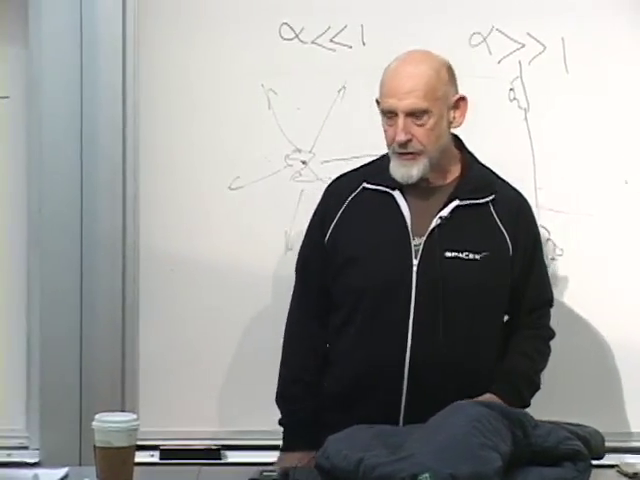
\includegraphics[width=0.72\textwidth]{lecture_01_figure_02.png}
\lectureframe{00:38:22.500}

\vspace{1em}

\begin{tikzpicture}[scale=0.95]
\draw (-5.3,-2.4) rectangle (-1.0,2.1);
\draw (0.3,-2.4) rectangle (4.6,2.1);

\node at (-3.15,2.55) {$\alpha \ll 1$};
\node at (2.45,2.55) {$\alpha \gg 1$};

\draw[line width=0.9pt] (-3.15,-0.15) circle (0.22);
\draw[->,line width=0.8pt] (-3.15,0.07) -- (-3.15,1.35);
\draw[->,line width=0.8pt] (-2.98,-0.01) -- (-1.95,1.00);
\draw[->,line width=0.8pt] (-3.32,-0.01) -- (-4.35,1.00);
\draw[->,line width=0.8pt] (-2.95,-0.23) -- (-1.80,-0.95);
\draw[->,line width=0.8pt] (-3.35,-0.23) -- (-4.50,-0.95);

\draw[line width=1.0pt] (2.15,-1.8) .. controls (1.95,-0.6) and (1.95,0.8) .. (2.15,1.55);
\draw[line width=1.0pt] (2.75,-1.8) .. controls (2.95,-0.6) and (2.95,0.8) .. (2.75,1.55);
\draw[line width=0.8pt] (2.15,-0.85) -- (2.75,-0.85);
\draw[line width=0.8pt] (2.45,1.55) -- (2.45,1.95);
\end{tikzpicture}\caption{Comparaison entre couplages faible--fort en électrodynamique quantique pendant la discussion sur l’énergie d’interaction. Le schéma isole les deux régimes évoqués par Susskind : un nuage dilué à faible couplage et un nuage proliférant à fort couplage.}\end{figure}

Cette figure a sa place ici parce que, même si la comparaison entre couplages faible--fort a été introduite plus tôt, Susskind reprend le contraste dans le cours à ce moment ultérieur, à l’occasion d’une question sur l’énergie d’interaction et la prolifération des structures.

\section{Théories à branes de dimension paire et émergence d’une dimension supplémentaire}

Jusqu’ici, le cours a développé l’idée d’échange : fermion contre boson, électron contre monopôle, corde F contre corde D. L’étape suivante est plus surprenante. Susskind passe à une autre version de la théorie des cordes, où les D-branes sont de dimension paire plutôt qu’impaire. Cette distinction compte, car dans cette théorie il n’y a pas de corde D à échanger contre la corde F. On y trouve des D0-branes, des D2-branes, des D4-branes, et ainsi de suite.

La limite de couplage fort ne peut donc pas se réduire à rebaptiser une corde. Selon le cours, il se passe quelque chose de plus étrange : une dimension spatiale supplémentaire devient manifeste. Susskind commence délibérément par la formulation la plus spectaculaire : ---``une nouvelle dimension apparaît''---, puis la reformule aussitôt avec davantage de précision : une direction compacte de très petite taille s’agrandit jusqu’à devenir impossible à négliger.

Le décompte fait partie du propos, aussi Susskind s’y arrête-t-il :
\begin{equation}
\begin{aligned}
10\text{-dimensional string theory} &= 9\text{ space}+1\text{ time},\\
11\text{-dimensional theory} &= 10\text{ space}+1\text{ time}.
\end{aligned}
\end{equation}
Selon le cours, la limite de couplage fort de la théorie à branes de dimension paire est effectivement une théorie à onze dimensions.

\editorialnote{La théorie à branes de dimension paire est la théorie des cordes de type IIA, dont le prolongement à couplage fort est la théorie M. Dans les unités usuelles, le rayon du cercle émergent et la longueur de Planck à onze dimensions varient comme \(R_{11}=g_s\ell_s\) et \(\ell_{11}=g_s^{1/3}\ell_s\). Ces noms et formules explicitent le dictionnaire moderne qui sous-tend la description géométrique du cours.}

\subsection{Le sandwich au beurre de cacahuète}

Pour se représenter la direction compacte, Susskind utilise le modèle du ``sandwich au beurre de cacahuète'' : deux tranches de pain infiniment minces, séparées par un véritable espace. La règle particulière est que sortir d’un côté fait réapparaître de l’autre. Dans une notation conventionnelle, que le cours illustre plutôt qu’il ne formule, on peut écrire
\begin{equation}
y \sim y + 2\pi R.
\end{equation}
Si \(R\) est très petit, les observateurs vivant dans le sandwich décrivent effectivement leur monde comme étant de dimension inférieure. L’effet essentiel du passage au couplage fort est alors
\begin{equation}
g\uparrow
\qquad \Longrightarrow \qquad
R_{\mathrm{compact}}\uparrow.
\end{equation}
Voilà ce que Susskind entend par l’apparition d’une nouvelle dimension spatiale : l’espace n’est pas créé à partir de rien ; une direction compacte jusque-là minuscule s’agrandit et devient visible dans la théorie effective.

\begin{figure}[htbp]\centering
\resizebox{\linewidth}{!}{%
\begin{tikzpicture}[scale=0.95]
\draw[line width=0.9pt] (-5,1.7) -- (5,1.7);
\draw[line width=0.9pt] (-5,-1.7) -- (5,-1.7);

\node[left] at (-5,1.7) {ceiling};
\node[left] at (-5,-1.7) {floor};

\draw[->,line width=0.8pt] (5.2,1.45) -- (5.2,-1.45);
\draw[->,line width=0.8pt] (5.5,-1.45) -- (5.5,1.45);
\node[right] at (5.55,0) {periodic};

\draw[line width=1.0pt] (-2.6,0.45) -- (2.2,0.45);
\draw[line width=1.0pt] (-2.6,-0.05) -- (2.2,-0.05);
\draw[line width=1.0pt] (-2.6,0.45) -- (-2.6,-0.05);
\draw[line width=1.0pt] (2.2,0.45) -- (2.2,-0.05);
\node at (-0.2,0.9) {floating D2-brane};

\draw[line width=1.0pt] (3.15,-1.7) -- (3.8,-1.7);
\draw[line width=1.0pt] (3.15,1.7) -- (3.8,1.7);
\draw[line width=1.0pt] (3.15,-1.7) -- (3.15,1.7);
\draw[line width=1.0pt] (3.8,-1.7) -- (3.8,1.7);
\node[right] at (3.95,0) {D2 ribbon};

\fill (-3.8,0) circle (0.07);
\node[below] at (-3.8,-0.05) {D0};
\end{tikzpicture}}%
\caption{Compactification en sandwich. Les bords supérieur et inférieur sont identifiés périodiquement ; une D2-brane flotte entre eux comme un tapis, tandis qu’une autre s’étend du sol au plafond et ressemble à une corde lorsque la direction compacte est de petite taille.}\end{figure}

\subsection{Que deviennent les D0- et D2-branes ?}

Le cours demande maintenant ce qui advient des D0-branes et des cordes. La réponse est asymétrique. Quand \(g\) devient grand, les D0-branes s’allègent de plus en plus ; dans l’interprétation en dimension supérieure, elles rejoignent la tour des particules porteuses de quantité de mouvement dans la direction nouvellement manifeste. Ainsi, un objet lourd et complexe dans la description à faible couplage devient une excitation ordinaire et légère dans celle à fort couplage.

La relation de masse explicite cette identification :
\begin{equation}
M_{D0}(n)=\frac{n}{g_s\ell_s}
=\frac{n}{R_{11}}
=M_{\mathrm{KK}}(n).
\end{equation}
\editorialnote{Susskind appelle les D0-branes « ``les gravitons'' » de la théorie à onze dimensions. Plus précisément, leurs états liés sont les modes de quantité de mouvement de Kaluza--Klein du multiplet de supergravité à onze dimensions, dont le secteur sans masse contient le graviton. Cette distinction conserve l’identification physique du cours sans aller jusqu’à affirmer littéralement qu’il s’agit d’une seule particule.}

Les D2-branes expliquent ce qu’il advient des cordes. Le cours met en avant deux configurations :
\begin{enumerate}
\item une D2-brane flottant entre le sol et le plafond comme un tapis dans le beurre de cacahuète ;
\item une D2-brane tendue du sol au plafond comme un ruban, étendu dans la direction visible.
\end{enumerate}
Lorsque le sandwich est mince, le ruban paraît effectivement unidimensionnel. C’est l’objet que les observateurs à basse énergie appellent une corde. À mesure que la direction compacte s’ouvre, ce même objet prend nettement la forme d’une membrane. Comme il s’étend désormais davantage dans la direction verticale, il devient lourd et ne ressemble plus à une corde.

\paragraph{La logique de la transition.}
\begin{enumerate}
\item Partons d’une direction compacte très mince, de sorte que le ruban vertical se comporte effectivement comme une corde.
\item Augmentons \(g\) : la direction compacte s’agrandit.
\item Les D0-branes s’allègent et sont réinterprétées comme des états de quantité de mouvement de Kaluza--Klein dans la théorie de dimension supérieure.
\item Le ruban de D2, semblable à une corde, devient une membrane visiblement étendue et s’alourdit.
\end{enumerate}
C’est le point d’articulation du cours entre dualité et géométrie émergente. Le couplage fort ne se contente pas d’échanger un objet contre un autre : il change la géométrie qui offre la description la plus efficace.

Susskind s’arrête sur l’étrangeté de cette idée. Le réseau d’identifications proposées exigeait de difficiles relations de cohérence mathématique, dont certaines ont d’abord été avancées par les physiciens sous forme de conjectures, puis démontrées par les mathématiciens. Il ne prétend pas que l’on comprend tous les vide de corde réalistes, mais que le réseau de dualités lui-même a résisté à des vérifications d’une rigueur inhabituelle.

Si le couplage varie d’un endroit à l’autre dans ce cadre idéalisé, la géométrie la plus efficace peut varier avec lui. Une région peut sembler presque de dimension dix, avec des cordes légères et des D0-branes lourdes ; une autre peut s’ouvrir sur la description de dimension onze, avec des membranes enroulées lourdes et des modes de Kaluza--Klein légers. Ce changement local de langage fait partie du même réseau de dualités.

La transcription rend brièvement le nom de ces relations par ``inégalités.'' Dans ce contexte, le mot visé est \emph{dualités} : des relations entre les deux extrémités opposées de l’espace des paramètres. Cette correction importe, car la conclusion de la leçon est précisément que l’on ne connaît aucune liste unique de constituants fondamentaux. Cordes, branes, particules et géométrie de dimension supérieure peuvent se transformer les uns dans les autres ; soit aucun élément du réseau n’est absolument fondamental, soit il existe une organisation plus profonde qui demeure inconnue.

\section{D3-branes, membranes enroulées et représentation géométrique de la dualité}

Après la pause, Susskind décrit explicitement le sujet comme un ``vaste réseau'' de théories et d’idées interconnectées. Les exemples qui suivent ne sont pas de nouveaux effets isolés ; ce sont des ponts qui relient les exemples précédents.

\subsection{Le volume d’univers d’une D3-brane}

Le premier pont fait intervenir une D3-brane. Une D3-brane possède trois dimensions spatiales et un observateur qui y est confiné peut facilement la prendre pour l’espace ordinaire. La brane peut se courber et fluctuer, tandis que les cordes qui s’y terminent peuvent se joindre, se scinder et diffuser. Pour un observateur qui ne voit que les directions le long de la brane, chaque extrémité ressemble à une particule et les interactions entre ces extrémités à celles d’une théorie quantique des champs ordinaire.

\begin{figure}[htbp]
\centering
\resizebox{\linewidth}{!}{%
\begin{tikzpicture}[scale=1.0]
\draw[fill=gray!15] (-4,-0.35) rectangle (4,0.35);
\node at (0,-0.75) {D3-brane};

\draw[line width=0.9pt] (-1.5,2.1) -- (-1.5,0.35);
\fill (-1.5,0.35) circle (0.07);
\node[left] at (-1.72,1.25) {F-string};
\node[below left] at (-1.5,0.32) {electric charge};

\draw[line width=1.5pt] (1.7,2.1) -- (1.7,0.35);
\fill (1.7,0.35) circle (0.09);
\node[right] at (1.95,1.25) {D-string};
\node[below right] at (1.7,0.32) {magnetic monopole};
\end{tikzpicture}
}%
\caption{Interprétation en termes de volume d’univers d’une D3-brane. L’extrémité d’une corde F apparaît comme une charge électrique ; celle d’une corde D apparaît comme un monopôle magnétique.}
\end{figure}

C’est l’une des identifications les plus satisfaisantes de la leçon. Pour l’observateur du volume d’univers, une corde F qui se termine sur la D3-brane apparaît comme une charge électrique. Une corde D se terminant sur cette même brane apparaît comme un monopôle magnétique. Autrement dit, sur le volume d’univers de la D3-brane, la dualité entre cordes F et cordes D devient la dualité électrique--magnétique de la théorie des champs ordinaire. Ce qui n’était auparavant qu’une analogie devient un dictionnaire explicite.

\editorialnote{Pour un empilement de D3-branes, la description à basse énergie sur le volume d’univers est une théorie de Yang--Mills supersymétrique en quatre dimensions, avec \(\mathcal N=4\). Sa dualité électrique--magnétique réalise, dans la théorie des champs, la dualité S de type IIB ; une brane unique donne la limite abélienne illustrée dans le cours.}

\subsection{Deux directions compactes et un enroulement asymétrique}

Susskind revient ensuite à la géométrie de dimension supérieure et compacte non pas une, mais deux petites directions. Comme on ne peut pas dessiner onze dimensions au tableau, il représente par une seule direction horizontale visible les sept grandes directions qui ne figurent pas dans le schéma, puis dessine explicitement les deux directions compactes. Il insiste sur l’asymétrie de la compactification : l’une des directions compactes doit être plus courte que l’autre pour que les cordes effectives aient des tensions différentes.

\begin{figure}[htbp]
\centering
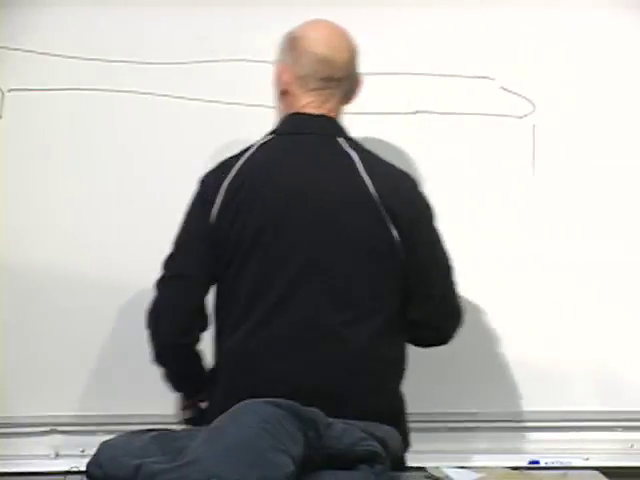
\includegraphics[width=0.78\textwidth]{lecture_01_figure_03.png}
\lectureframe{01:10:25.000}
\caption{État final du schéma au tableau pour les deux membranes enroulées. Les cycles compact court et long produisent les rubans de type corde F et corde D dessinés à droite.}
\end{figure}

Une membrane peut s’enrouler autour de l’une ou l’autre des directions compactes et apparaître comme une corde dans les directions non compactes. Si \(R_1\) et \(R_2\) sont les rayons des deux cercles, ses tensions effectives sont
\begin{equation}
\begin{aligned}
T_{(1)}&=2\pi R_1 T_{\mathrm{M2}},\\
T_{(2)}&=2\pi R_2 T_{\mathrm{M2}},\\
\frac{T_{(1)}}{T_{(2)}}&=\frac{R_1}{R_2}.
\end{aligned}
\end{equation}
Ainsi, des cercles de tailles différentes produisent des tensions de corde différentes. En identifiant l’enroulement le plus court à la corde F légère et le plus long à la corde D lourde, on peut écrire schématiquement
\begin{equation}
g_s\sim \frac{R_{\mathrm{short}}}{R_{\mathrm{long}}},
\qquad
\frac{T_{\mathrm{D1}}}{T_{\mathrm{F1}}}\sim \frac{1}{g_s}.
\end{equation}

\begin{classroomqa}
\audiencequestion{Dans ce schéma, le couplage peut-il s’interpréter comme le rapport des deux dimensions compactes ? \lecturetimestamp{01:10:13}}
\lecturerresponse{Oui. Le paramètre faible--fort est géométrisé sous la forme d’un rapport d’aspect. Rendre une direction plus courte donne un faible couplage ; échanger les deux directions revient à échanger les cordes légère et lourde.}
\end{classroomqa}

\editorialnote{Dans la leçon, ce rapport est provisoirement noté \(\alpha\), le symbole précédemment utilisé pour la constante de structure fine de l’électrodynamique quantique. Nous écrivons ici \(g_s\) pour distinguer les deux significations. Dans la construction complète de la théorie M, le couplage de type IIB est encodé dans la structure complexe du tore compact à deux dimensions ; le numérateur précis dépend de la manière dont ses cycles sont étiquetés.}

On peut résumer la représentation par membranes enroulées sans la distorsion de perspective du dessin au tableau :

\begin{figure}[htbp]
\centering
\begin{tikzpicture}[scale=1.0]
\draw[line width=0.9pt] (0,0) rectangle (5.2,2.2);
\node[below] at (2.6,-0.2) {\(R_1\)};
\node[right] at (5.4,1.1) {\(R_2\)};

\draw[->,line width=0.7pt] (5.45,1.9) -- (5.45,0.3);
\draw[->,line width=0.7pt] (5.7,0.3) -- (5.7,1.9);
\draw[->,line width=0.7pt] (0.4,-0.35) -- (4.8,-0.35);
\draw[->,line width=0.7pt] (4.8,-0.6) -- (0.4,-0.6);

\draw[line width=1.0pt] (1.1,0) -- (1.6,0) -- (1.6,2.2) -- (1.1,2.2) -- cycle;
\node at (1.35,2.55) {light};

\draw[line width=1.0pt] (0,1.45) -- (5.2,1.45);
\draw[line width=1.0pt] (0,1.00) -- (5.2,1.00);
\node at (4.55,1.95) {heavy};

\node at (1.35,-0.95) {F-string};
\node at (4.55,0.55) {D-string};
\end{tikzpicture}
\caption{Deux configurations de membranes enroulées semblent toutes deux être des cordes dans les directions non compactes, mais la différence d’échelle des directions compactes rend l’une des cordes effectives plus légère que l’autre.}
\end{figure}

C’est la version géométrique du récit de dualité précédent. Comprimer une direction tout en étirant l’autre alourdit un objet enroulé et allège l’autre, de sorte que les rôles des cordes F et D peuvent s’inverser.

\begin{classroomqa}
\audiencequestion{Si les directions compactes sont cycliques, les objets enroulés sont-ils infiniment larges ? \lecturetimestamp{01:10:41}}
\lecturerresponse{Non. Un cercle compact a une circonférence finie, même si l’on peut le parcourir indéfiniment sans rencontrer de bord. Le haut et le bas du dessin déroulé représentent le même point, tout comme les extrémités d’un intervalle peuvent représenter un seul point d’un cercle.}
\end{classroomqa}

\begin{figure}[htbp]
\centering
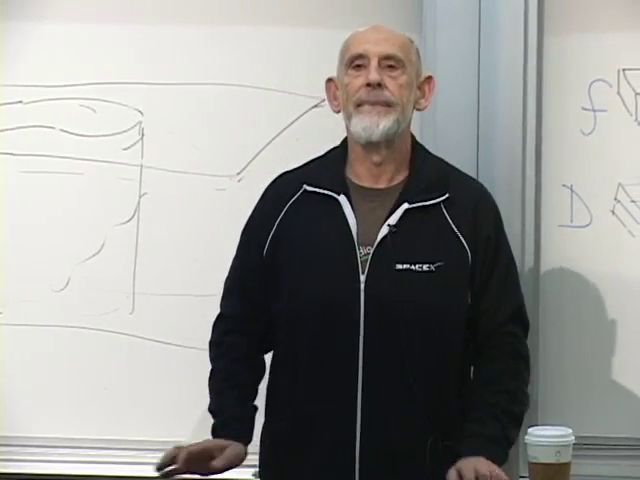
\includegraphics[width=0.78\textwidth]{lecture_01_figure_04.png}
\lectureframe{01:12:25.000}

\vspace{1em}

\begin{tikzpicture}[scale=0.95]
\draw[line width=0.9pt,->] (-3.7,0) arc[start angle=180,end angle=535,radius=0.95];
\node at (-2.75,0) {compact circle};
\draw[line width=0.9pt] (0.0,0) -- (4.8,0);
\fill (0.0,0) circle (0.06);
\fill (4.8,0) circle (0.06);
\draw[<->] (0.0,-0.45) -- (4.8,-0.45);
\node at (2.4,-0.75) {cut-open interval of length \(2\pi R\)};
\node[above] at (0.0,0.1) {same point};
\node[above] at (4.8,0.1) {same point};
\end{tikzpicture}
\caption{Un cercle compact et sa représentation déroulée au tableau. En franchissant une extrémité, on revient par l’autre ; se déplacer autour du cercle tout en avançant dans une direction non compacte tracerait plutôt une hélice.}
\end{figure}

\begin{classroomqa}
\audiencequestion{Pourquoi le chemin compact est-il un cercle plutôt qu’une hélice ? \lecturetimestamp{01:12:23}}
\lecturerresponse{En chaque point fixe de la direction non compacte, la direction compacte est un cercle. Une hélice n’apparaît que si l’on avance dans la direction non compacte tout en s’enroulant autour du cercle. L’intervalle dessiné au tableau est simplement un cercle coupé, dont les deux extrémités sont identifiées.}
\end{classroomqa}

\begin{classroomqa}
\audiencequestion{Cette géométrie explique-t-elle à elle seule comment une D-brane peut ressembler à un ensemble de cordes F lorsqu’on la sonde de près ? \lecturetimestamp{01:12:49}}
\lecturerresponse{Le lien existe, mais il n’est pas manifeste dans cette représentation élémentaire ; il faut un outillage géométrique plus élaboré pour le voir. Le schéma sert à organiser la dualité, pas à dériver la description de tous les constituants microscopiques.}
\end{classroomqa}

\begin{classroomqa}
\audiencequestion{Les directions compactes longue et courte peuvent-elles s’échanger lorsqu’on se déplace dans l’espace ou au cours du temps ? \lecturetimestamp{01:13:35}}
\lecturerresponse{L’un ou l’autre est possible dans le modèle idéalisé. Comprimer un cycle tout en dilatant l’autre inverse lequel des cordes enroulées est léger. C’est une autre raison pour laquelle ``corde fondamentale'' n’est qu’un nom : la description privilégiée peut changer d’une région à l’autre ou au cours du temps.}
\end{classroomqa}

\section{Idéalisation, points de symétrie particulière et paysage}

Dans le dernier mouvement de la leçon, Susskind prend du recul par rapport aux élégants exemples de dualité et se demande ce qu’ils nous apprennent — et ce qu’ils ne nous apprennent pas — sur le monde réel.

Tout d’abord, Susskind avertit que les dualités précisément contrôlées sont des propriétés de théories supersymétriques fortement idéalisées, dans lesquelles bosons et fermions ont des masses exactement égales. Il les compare aux orbites circulaires de la mécanique newtonienne : on les étudie d’abord parce qu’elles sont symétriques et mathématiquement faciles à traiter, non parce que le mouvement réel des planètes se réduit à des cercles parfaits. De même, les théories des cordes supersymétriques sont plus faciles à analyser parce qu’elles sont plus symétriques que ne semble l’être la nature.

Cette idéalisation n’en est pas moins instructive. Une orbite circulaire parfaite ne représente pas un système planétaire réaliste, mais elle met en évidence des propriétés qui subsistent pour des orbites moins symétriques. De même, les exemples supersymétriques montrent des façons cohérentes d’articuler la mécanique quantique, la gravité et la structure microscopique. Susskind formule délibérément les choses de manière tranchée : littéralement, les théories des cordes traitables ne sont pas la théorie de notre monde ; elles sont utiles parce qu’elles révèlent des phénomènes susceptibles de réapparaître dans des cadres moins symétriques et moins faciles à traiter.

\subsection{Un ensemble de briques de construction aux nombreuses issues}

Les D-branes ne sont qu’un élément de l’ensemble de briques de construction disponible. La leçon mentionne aussi les flux, les orbifolds et les orientifolds. On choisit d’abord une géométrie compacte, puis les branes et les flux qui occupent ses cycles. Même le simple sandwich change de physique à basse dimension lorsqu’on y insère une, deux ou trois D2-branes flottantes. Ajouter ou retirer de tels ingrédients modifie les particules, les interactions et les paramètres effectifs.

Supposons que, dans le décompte schématique de la leçon, un espace compact à six dimensions possède environ \(500\) cycles, et que chaque cycle admette de l’ordre de \(10\) possibilités de branes enroulées, de flux ou de structures apparentées. Le nombre de constructions croît alors comme
\begin{equation}
N_{\mathrm{vacua}} \sim 10^{500}.
\end{equation}
Le raisonnement de la leçon est élémentaire :
\begin{equation}
10 \times 10 \times \cdots \times 10 = 10^{500}
\end{equation}
avec \(500\) facteurs. L’analogie avec l’ADN exprime la même idée dans un registre plus familier :
\begin{equation}
N_{\mathrm{DNA}}(500)=4^{500}.
\end{equation}
Lors de la comparaison avec l’ADN, un membre du public vérifie qu’il y a quatre possibilités le long d’un brin : A, C, G et T. Cette correction renforce l’argument sans le modifier. Une courte liste de choix locaux, répétée de nombreuses fois, produit un nombre immense d’arrangements globaux. L’exposant exact n’est pas le point essentiel, et Susskind qualifie \(10^{500}\) de vieille sous-estimation ; l’essentiel est la prolifération combinatoire.

On aboutit ainsi à l’inversion finale de l’attente réductionniste formulée au début. Une physique des particules complexe ne nécessite pas forcément des règles microscopiques complexes. Elle peut résulter du fait que notre vide est un arrangement complexe de nombreux ingrédients simples, tout comme un organisme complexe peut être encodé par une séquence constituée de quatre bases.

\begin{classroomqa}
\audiencequestion{Une fois identifiées les descriptions équivalentes liées par dualité, une connaissance complète permettrait-elle de ne retenir qu’un seul de ces vides possibles, ou quelques-uns, comme descriptions de notre monde ? \lecturetimestamp{01:26:11}}
\lecturerresponse{On peut présumer qu’elle sélectionnerait un ensemble restreint, mais de nombreux vides distincts pourraient sembler extrêmement semblables aux énergies accessibles. Le nombre cité pour le paysage est censé rester élevé même après identification des descriptions duales, et les détails de haute énergie sans pertinence pourraient jouer le rôle de ``l’ADN poubelle.''}
\end{classroomqa}

\subsection{Points de symétrie et complexité générique}

Dans le paysage, il existe des points présentant une symétrie particulière. Dans la représentation géométrique, une configuration de rapport d’aspect égal,
\begin{equation}
R_1=R_2,
\end{equation}
rend les deux descriptions par enroulement aussi simples l’une que l’autre. Dans l’analogie électrique--magnétique, cela se représente schématiquement par
\begin{equation}
m_{\mathrm{monopole}}=m_e.
\end{equation}

\begin{figure}[htbp]
\centering
\begin{tikzpicture}[scale=0.95]
\draw[line width=0.9pt] (-4.5,-1.0) rectangle (-2.5,1.0);
\draw[<->] (-4.5,-1.35) -- (-2.5,-1.35);
\draw[<->] (-2.15,-1.0) -- (-2.15,1.0);
\node at (-3.5,1.45) {symmetric point};
\node at (-3.5,-1.75) {$R_1=R_2$};

\draw[line width=0.9pt] (0.0,-0.55) rectangle (4.8,0.55);
\draw[<->] (0.0,-0.9) -- (4.8,-0.9);
\draw[<->] (5.15,-0.55) -- (5.15,0.55);
\node at (2.4,1.45) {lopsided point};
\node at (2.4,-1.3) {$R_1\ne R_2$};
\end{tikzpicture}
\caption{Une compactification de rapport d’aspect égal traite symétriquement les deux cordes enroulées ; une compactification dissymétrique rend l’une des descriptions beaucoup plus légère que l’autre.}
\end{figure}

\begin{classroomqa}
\audiencequestion{Existe-t-il dans le paysage des vides où la construction devient beaucoup plus simple parce que les descriptions en termes de cordes F et D coïncident ? \lecturetimestamp{01:27:21}}
\lecturerresponse{Oui, il existe des points présentant une symétrie particulière. Notre monde ne semble pas se trouver en l’un d’eux : la particule électrique familière et le monopôle magnétique n’ont pas la même masse. On ignore pourquoi la nature occupe un point dissymétrique.}
\end{classroomqa}

\editorialnote{L’égalité des masses de l’électron et du monopôle-- est une propriété schématique d’un modèle autodual convenablement protégé, et non une prédiction de l’électrodynamique quantique ordinaire non supersymétrique. Elle exprime l’idée du point de symétrie de la leçon, sans prétendre décrire l’électron observé.}

Susskind évoque ensuite une analogie issue de la théorie de la communication. Les codes aléatoires peuvent être extraordinairement efficaces, tandis que ceux qui sont les plus faciles à décrire et à décoder possèdent une structure mathématique supplémentaire et ont historiquement donné de moins bons résultats. La théorie du codage a ensuite trouvé des constructions structurées très efficaces, mais l’analogie reste valable : tout ce que l’on peut nommer ou décrire de façon concise occupe un coin très particulier, de faible complexité, de l’espace complet des possibilités. De même, les vides de corde les plus faciles à calculer peuvent être atypiquement simples.

Les questions pertinentes pourraient donc changer. Au lieu d’exiger la compactification exacte jusque dans chaque détail microscopique, on peut se demander quelles propriétés sont courantes ou génériques dans un vaste ensemble. Susskind présente cela comme un problème de recherche, et non comme une conclusion établie, et rejette les arguments idéologiques qui se substitueraient au calcul.

\subsection{Questions cosmologiques}

\begin{classroomqa}
\audiencequestion{Une direction compacte de circonférence énorme est-elle différente, du point de vue observationnel, d’une direction infinie ? Savons-nous que nos trois grandes dimensions spatiales sont infinies ? \lecturetimestamp{01:30:03}}
\lecturerresponse{Nous ne savons pas qu’elles sont infinies. Une trois-sphère fermée peut se dilater tout en restant compacte. Les mesures de la quasi-planéité ne donnent qu’une borne inférieure du rayon de courbure, de même que l’arpentage d’un terrain presque plat peut fournir une borne sur la taille de la Terre sans prouver que sa surface est infinie. Seule la détection d’une courbure ou d’une identification globale permettrait de déterminer l’échelle finie.}
\end{classroomqa}

\begin{classroomqa}
\audiencequestion{Si le couplage peut varier dans l’espace au sein du modèle idéalisé, comment une telle variation pourrait-elle se produire dans le monde réel ? \lecturetimestamp{01:32:43}}
\lecturerresponse{Pas sous la forme de la variation lisse et sans restriction utilisée dans l’exemple symétrique. La possibilité réaliste qui sera examinée plus loin est une variation par transitions discrètes entre des régions régies par des lois effectives différentes. La question de savoir si de tels sauts se produisent est une question cosmologique.}
\end{classroomqa}

\editorialnote{Cette réponse doit être comprise comme un aperçu, dans la leçon, des vides de flux et des transitions entre domaines, et non comme un théorème général interdisant tout champ scalaire variant de façon lisse. Les observations contraignent fortement les variations des couplages sans dimension, tandis que les mécanismes de stabilisation déterminent si des modules continus restent possibles dans un modèle donné.}

L’enregistrement ne conserve pas la dernière question du public. La réponse qui subsiste indique que le phénomène proposé peut se produire pour certains types de trous noirs, mais pas à l’horizon d’un trou noir de Schwarzschild ordinaire, dont l’horizon est, localement, un lieu ordinaire pour un observateur en chute libre. Comme il est impossible de reconstituer la question de manière fiable, aucun propos plus précis n’est attribué à cet échange.

\section{Des briques à un réseau de descriptions}

L’espoir que les couches les plus profondes de la physique soient nécessairement plus simples s’est révélé fragile. En bosonisation en \(1+1\) dimensions, une même théorie peut être formulée soit en termes de fermions, soit en termes de bosons, le fermion réapparaissant sous la forme d’un kink. En électrodynamique quantique, les couplages faible et fort échangent les rôles descriptifs de l’électron et du monopôle magnétique. En théorie des cordes, les cordes F et les cordes D répètent le même schéma ; dans la théorie des branes de dimension paire, le couplage fort va encore plus loin : une direction compacte s’agrandit, les D0-branes deviennent des états de quantité de mouvement de Kaluza--Klein, et les cordes effectives sont réinterprétées comme des membranes enroulées dans une géométrie de dimension supérieure. La théorie quantique des champs moderne et la théorie des cordes n’apportent donc pas de réponse unique et définitive à la question ``quelles sont les briques et quelles sont les maisons ?'' Elles offrent un réseau de descriptions, chacune efficace dans son propre régime, ainsi qu’un immense paysage de constructions possibles dont le résultat générique est la complexité plutôt que la simplicité.

\chapter{Géométrie, information et loi de l’aire des trous noirs}

\lectureoverview{La destination annoncée est la cosmologie, mais le chemin le plus court pour y parvenir commence par un retour à la relativité restreinte. Une métrique décrit la géométrie de l’espace-temps, et la condition de temps propre nul indique comment se propage la lumière. Nous appliquerons cette règle à la géométrie de Schwarzschild, distinguerons l’horizon de la singularité, puis nous demanderons ce qu’il advient de l’information lorsqu’un trou noir rayonne et s’évapore. La réponse part de l’entropie ordinaire et aboutit à l’argument de Bekenstein fondé sur un bit : un trou noir stocke l’information par unités d’aire de l’horizon, et non de volume.}

Susskind reporte brièvement le bilan promis des succès et des échecs de la théorie des cordes. Il est tard, dit-il, et il vaut mieux parler du fond que faire un bilan. Ce soir, le fond consiste dans la géométrie et la thermodynamique minimales nécessaires pour poser le problème de l’information des trous noirs.

\section{Une règle pour la lumière}

La relativité restreinte traite l’espace et le temps comme un seul objet géométrique. Pour des événements voisins séparés par \(dt,dx,dy,dz\), Susskind adopte la convention où le signe temporel est positif et écrit
\begin{equation}
d\tau^2=dt^2-\frac{1}{c^2}\left(dx^2+dy^2+dz^2\right).
\end{equation}
Les signes opposés des termes temporel et spatial distinguent la géométrie de Minkowski de la géométrie euclidienne à quatre dimensions. Le facteur \(1/c^2\) ne sert qu’à rendre les unités compatibles ; en mesurant le temps et la distance de façon cohérente, on peut poser \(c=1\).

Pour une séparation de genre temps, \(d\tau^2>0\), et \(d\tau\) est le temps propre indiqué par une horloge qui suit la trajectoire. Les séparations de genre espace vérifient plutôt \(d\tau^2<0\). Le cas qui nous intéresse ce soir se situe exactement entre les deux. Un rayon lumineux suit une trajectoire \emph{nulle},
\begin{equation}
d\tau^2=0.
\end{equation}
En se limitant d’abord au mouvement selon l’axe \(x\), on obtient
\begin{align}
0&=dt^2-\frac{dx^2}{c^2},\\
c\,dt&=\pm dx,\\
\frac{dx}{dt}&=\pm c.
\end{align}
Les signes décrivent les rayons qui se propagent vers la droite et vers la gauche. La valeur numérique attribuée à \(c\) change lorsqu’on remplace les centimètres par des mètres ou des kilomètres ; l’énoncé invariant n’est pas un nombre, mais la condition de nullité.

En relativité générale, c’est la métrique qui se complique, pas cette règle. Avec les coordonnées \(x^\mu\), \(\mu=0,1,2,3\),
\begin{equation}
ds^2=g_{\mu\nu}(x)\,dx^\mu dx^\nu,
\end{equation}
où les indices répétés sont sommés et où les coefficients peuvent varier d’un point à l’autre. Pour trouver les directions localement accessibles à la lumière, on annule cette forme quadratique.

\section{Coordonnées sphériques et métrique de Schwarzschild}

Un trou noir non rotatif est à symétrie sphérique ; les coordonnées cartésiennes en masquent donc la structure utile. Soit \(r\) la distance radiale et \(\theta,\phi\) les coordonnées d’une direction sur une sphère unité. Son élément de ligne est
\begin{equation}
d\Omega^2=d\theta^2+\sin^2\theta\,d\phi^2.
\end{equation}
Sur une sphère de rayon \(r\), les déplacements angulaires contribuent donc par \(r^2d\Omega^2\). L’espace-temps plat en coordonnées sphériques s’écrit
\begin{equation}
d\tau^2=dt^2-\left(dr^2+r^2d\Omega^2\right),
\qquad (c=1).
\end{equation}

Susskind ne dérive pas la solution du trou noir à partir des équations d’Einstein. Il l’écrit et nous invite à l’examiner. Le tableau rend explicite la comparaison recherchée.

\begin{figure}[htbp]
\centering
\includegraphics[width=0.86\textwidth]{lecture_02_figure_02.png}
\caption{L’espace-temps plat en coordonnées sphériques, au-dessus de la déformation de Schwarzschild. Le facteur répété \(1-2GM/(c^2r)=1-R_s/r\) et le schéma radial apparaissent ensemble.}
\lectureframe{00:19:12.520}
\end{figure}

Pour un trou noir de masse \(M\), définissons le rayon de Schwarzschild
\begin{equation}
R_s=\frac{2GM}{c^2}.
\end{equation}
L’élément de ligne extérieur est
\begin{equation}
d\tau^2=\left(1-\frac{R_s}{r}\right)dt^2
-\frac{dr^2/c^2}{1-R_s/r}
-\frac{r^2}{c^2}d\Omega^2.
\label{eq:schwarzschild-explicit-c}
\end{equation}
De manière équivalente, en posant \(c=1\),
\begin{equation}
ds^2=\left(1-\frac{2GM}{r}\right)dt^2
-\frac{dr^2}{1-2GM/r}-r^2d\Omega^2.
\label{eq:schwarzschild}
\end{equation}
Loin du trou noir, \(R_s/r\ll1\), et l’on retrouve la métrique sphérique plate. Cette vérification asymptotique importe davantage que de mémoriser la formule, même si Susskind recommande cette dernière comme sujet de conversation lors des cocktails.

\editorialnote{Le tableau alterne entre \(d\tau^2\) et \(ds^2\), et n’affiche pas toujours de manière cohérente tous les facteurs de \(c\). L’équation~\eqref{eq:schwarzschild-explicit-c} suit la convention de la conférence pour la coordonnée temporelle, dans laquelle \(t\) a la dimension d’un temps. La forme standard avec \(x^0=ct\) lui est algébriquement équivalente.}

\subsection{L’horizon n’est pas la singularité}

Dans ces coordonnées, deux rayons semblent suspects. En \(r=R_s=2GM\), en unités naturelles, le coefficient de \(dt^2\) s’annule et celui de \(dr^2\) diverge. En \(r=0\), la courbure elle-même devient singulière. Il ne s’agit pas de deux versions d’un même événement :
\begin{equation}
\begin{aligned}
r=R_s &:\quad \text{horizon},\\
r=0 &:\quad \text{curvature singularity}.
\end{aligned}
\end{equation}

Les forces de marée permettent de distinguer physiquement les deux cas. Un champ gravitationnel varie d’un point à l’autre d’un corps étendu : les pieds peuvent être attirés plus fortement que la tête, ce qui étire le corps tandis que les directions transversales sont comprimées. À l’horizon, ces forces de marée restent finies ; à l’horizon d’un trou noir suffisamment massif, elles peuvent être très faibles. Rien de catastrophique ne doit nécessairement s’y produire localement. En revanche, en \(r=0\), les forces de marée divergent. Les coefficients inquiétants en \(r=R_s\) signalent un défaut des coordonnées de Schwarzschild ; la singularité en \(r=0\) est physique.

\editorialnote{On peut vérifier que la courbure reste finie en \(r=R_s\) à l’aide du scalaire de Kretschmann \(R_{\mu\nu\rho\sigma}R^{\mu\nu\rho\sigma}=48G^2M^2/(c^4r^6)\), qui est fini à l’horizon et ne diverge que lorsque \(r\to0\). Cet invariant n’a pas été écrit pendant la conférence, mais il précise la distinction entre les forces de marée.}

\section{La lumière radiale près de l’horizon}

Revenons maintenant à notre règle. Un rayon radial conserve sa position angulaire, donc \(d\Omega=0\), et un rayon lumineux vérifie \(ds^2=0\). En unités où \(c=1\), l’équation~\eqref{eq:schwarzschild} donne
\begin{equation}
0=\left(1-\frac{2GM}{r}\right)dt^2
-\frac{dr^2}{1-2GM/r}.
\end{equation}
En multipliant par \(1-2GM/r\) et en prenant la racine carrée, on obtient deux branches,
\begin{align}
dr&=\pm\left(1-\frac{2GM}{r}\right)dt,\\
\frac{dr}{dt}&=\pm\left(1-\frac{2GM}{r}\right).
\label{eq:radial-null}
\end{align}
Le signe plus correspond à la propagation vers l’extérieur, le signe moins à la propagation vers l’intérieur. Loin du trou noir, leurs vitesses coordonnées tendent vers \(\pm1\). À l’horizon, les deux vérifient \(\lvert dr/dt\rvert\to0\) : en temps coordonné de Schwarzschild, un rayon sortant semble s’y immobiliser, tandis qu’un rayon entrant met un temps coordonné infini à l’atteindre.

\begin{figure}[htbp]
\centering
\includegraphics[width=0.82\textwidth]{lecture_02_figure_03.png}
\caption{Schéma complété au tableau en coordonnées \(t\)-\(r\) : les rayons nuls radiaux deviennent presque verticaux à mesure qu’ils approchent de l’horizon en pointillés.}
\lectureframe{00:30:25.000}
\end{figure}

\begin{figure}[htbp]
\centering
\begin{tikzpicture}[x=1.0cm,y=0.9cm]
\draw[->] (0,0) -- (6.6,0) node[right] {$r$};
\draw[->] (0,0) -- (0,6.2) node[above] {$t$};
\draw[dashed,thick] (2.0,0) -- (2.0,5.9) node[above] {$r=R_s$};
\draw[thick,->] (2.08,.4) .. controls (2.10,2.2) and (2.55,3.8) .. (5.8,5.7);
\draw[thick,->] (5.8,.5) .. controls (3.2,2.0) and (2.15,4.2) .. (2.03,5.7);
\node[align=center] at (4.7,4.4) {outgoing};
\node[align=center] at (4.5,1.2) {ingoing};
\end{tikzpicture}
\caption{Version épurée du schéma au tableau en temps coordonné. Le ralentissement apparent concerne \(t\) de Schwarzschild, et non un défaut local de propagation de la lumière à \(c\).}
\end{figure}

À l’intérieur de l’horizon, les cônes de lumière futurs s’inclinent si fortement vers l’intérieur que les deux branches radiales orientées vers le futur conduisent à des valeurs décroissantes de \(r\). Aucun signal émis depuis cette région ne peut s’échapper vers l’extérieur, et toute trajectoire causale orientée vers le futur atteint la singularité.

\begin{classroomqa}
\audiencequestion{Si la vitesse de la lumière est invariante, que signifie exactement l’affirmation selon laquelle la lumière ralentit près de l’horizon ?\lecturetimestamp{00:31:44}}
\lecturerresponse{La quantité affichée est \(dr/dt\) dans un système de coordonnées particulier. La valeur numérique d’une vitesse change déjà lorsqu’on remplace les mètres par des centimètres ; ici, les étalons radiaux et temporels effectifs varient selon la position. L’énoncé universel est que tout rayon lumineux suit une trajectoire nulle, \(ds^2=0\).}
\end{classroomqa}
\editorialnote{Un observateur local en chute libre mesure la vitesse de la lumière dans le vide comme étant \(c\) ; la vitesse nulle en coordonnées de Schwarzschild à l’horizon n’est pas une grandeur observable localement.}

\begin{classroomqa}
\audiencequestion{La même affirmation sur la vitesse nulle vaut-elle quel que soit le milieu matériel dans lequel la lumière se propage ?\lecturetimestamp{00:33:24}}
\lecturerresponse{Non. La reconnaissance disponible ne conserve pas d’explication plus détaillée de cette réponse.}
\end{classroomqa}
\editorialnote{L’affirmation concernant la vitesse de la lumière nulle porte sur sa propagation dans l’espace-temps vide. Les interactions avec la matière peuvent donner à un paquet d’ondes une vitesse effective plus faible ; c’est une propriété du milieu, pas une modification de la vitesse causale locale \(c\).}

\begin{classroomqa}
\audiencequestion{À quoi ressemble un rayon lumineux entrant sur le même diagramme \(t\)-\(r\) ?\lecturetimestamp{00:33:32}}
\lecturerresponse{C’est la branche qui semble suivre le trajet inverse : partant d’une grande valeur de \(r\), elle se courbe vers l’horizon et s’en approche asymptotiquement. Il lui faut un temps coordonné infini \(t\) pour l’atteindre.}
\end{classroomqa}
\editorialnote{Un observateur en chute libre atteint et franchit l’horizon en un temps propre fini ; seul \(t\) de Schwarzschild diverge.}

\section{Pourquoi l’évaporation pose un problème}

L’horizon mérite une étude bien plus approfondie : comment il se forme, ce que voit un observateur en chute libre, et si quelque chose d’inhabituel s’y produit localement. Susskind remet ces questions à plus tard et passe à la mécanique quantique. Du point de vue extérieur, la matière et toutes les informations qui permettent de la distinguer se trouvent comprimées toujours plus près de l’horizon et deviennent inaccessibles. Cela seul n’implique pas nécessairement une destruction de l’information ; elle peut simplement être cachée.

Le résultat de Hawking rend le problème aigu. Un trou noir classique qui a atteint un état stationnaire semble être l’objet le plus terne qui soit : sphérique, sombre et incapable d’envoyer un message. Mais ``noir'' a deux sens. Le mot peut signifier qu’il n’émet rien, ou qu’il émet un rayonnement thermique de corps noir. Un trou noir quantique est noir dans ce second sens. Il a une température, brille et perd de l’énergie. Puisque
\begin{equation}
E=Mc^2,
\qquad
R_s=\frac{2GM}{c^2},
\end{equation}
le rayonnement diminue à la fois sa masse et le rayon de son horizon. Si l’évaporation finit par faire disparaître le trou noir, qu’advient-il de l’information qui semblait rester à son horizon ? Elle pourrait être détruite, piégée dans un minuscule résidu, ou encodée dans le rayonnement sortant. La tension entre ces possibilités constitue le problème de l’information, et la théorie des cordes nous aidera plus tard à en préciser la résolution.

Ce soir, aucun calcul de théorie quantique des champs en espace-temps courbe n’est entrepris. Susskind suit plutôt la voie plus simple de Bekenstein : d’abord comprendre l’entropie comme une information, puis calculer quelle quantité d’information un trou noir peut dissimuler.

\section{Une information présente, mais cachée}

Imaginons qu’on divise une boîte en cellules suffisamment petites pour que chacune soit occupée ou vide. Une chaîne binaire---une réponse par cellule---distingue cette configuration de toutes les autres configurations permises. Pour décrire la matière de façon plus réaliste, il faut aussi poser des questions sur les espèces de particules et d’autres degrés de liberté, mais le principe reste le même : l’information se mesure par le nombre minimal de questions oui--non nécessaires pour spécifier l’état.

\begin{classroomqa}
\audiencequestion{S’agit-il uniquement d’une description d’un système statique ?\lecturetimestamp{00:45:49}}
\lecturerresponse{C’est une description instantanée, à un instant donné. La dynamique transforme ensuite cet état en un autre état.}
\end{classroomqa}

Le principe suivant est plus profond : l’évolution d’un système fermé ne fusionne pas deux états microscopiques distincts en un seul. Si deux configurations diffèrent maintenant, leurs configurations après évolution restent distinguables en principe. L’évolution hamiltonienne classique est inversible et l’évolution quantique est unitaire.\editorialnote{Les équations effectives dissipatives ne peuvent effacer des distinctions que parce que les degrés de liberté de l’environnement, qui ne sont pas observés, ont été omis ; l’état complet du système fermé les conserve.}

La baignoire rend concrète la différence entre perte et inaccessibilité. Deux suites de gouttes pourraient coder deux textes distincts en code Morse. Une fois l’eau au repos, les deux baignoires semblent identiques. Les ondulations visibles ont disparu, mais une mesure microscopique complète révélerait encore des configurations moléculaires différentes. Le message s’est dispersé parmi des degrés de liberté trop petits et trop nombreux pour être suivis.

L’entropie correspond à cette information cachée. Au regard des questions macroscopiques que nous pouvons poser---température, énergie totale, composition, niveau de l’eau---, de nombreuses distinctions microscopiques restent possibles mais inaccessibles. Dans le décompte des bits utilisé pendant la conférence,
\begin{equation}
S=\hbox{number of hidden bits}.
\end{equation}
La formule statistique précise est \(S=k_B\ln\Omega\), mais la définition qualitative suffit pour l’argument sur les trous noirs.

\section{La température, coût de la dissimulation d’un bit}

La température est facile à mesurer, mais sa définition est étonnamment indirecte. Susskind prend l’entropie et l’énergie comme concepts fondamentaux. Supposons qu’un ordinateur réinitialise un bit à une valeur standard. Le dispositif physique subsiste, mais la distinction entre ses états antérieurs zéro et un disparaît de l’ordinateur. Elle ne peut disparaître du monde physique complet ; elle est transférée à des degrés de liberté microscopiques de l’environnement, qui s’échauffe légèrement. C’est le principe de Landauer.

Si une unité d’entropie correspond à un bit et que la température se mesure en unités d’énergie, la conférence écrit
\begin{align}
\Delta S&=1,\\
\Delta E&=T\,\Delta S,\\
dE&=T\,dS.
\label{eq:first-law}
\end{align}

\begin{figure}[htbp]
\centering
\includegraphics[width=0.84\textwidth]{lecture_02_figure_04.png}
\caption{La thermodynamique de l’information au tableau : \(S\) est l’entropie, un bit caché correspond à \(\Delta S=1\) et son coût énergétique minimal s’écrit \(\Delta E=T\Delta S\).}
\lectureframe{00:58:40.000}
\end{figure}

\editorialnote{En unités conventionnelles, le coût réversible d’effacement d’un bit binaire est \(k_BT\ln2\). L’équation~\eqref{eq:first-law} utilise \(k_B=1\) et traite l’unité d’entropie de la conférence comme un bit, tout en omettant le facteur \(\ln2\) correspondant. Ces conventions n’affectent pas l’argument d’échelle qui suit.}

Selon l’estimation avancée par une personne dans le public, la hausse minimale de température provoquée par l’effacement d’environ \(100\) gigaoctets dans un verre d’eau est proche de \(10^{-15}\) degrés. Susskind retient l’idée plutôt que le nombre exact : à température ambiante, l’énergie minimale associée à un bit est extraordinairement faible, et les ordinateurs réels dissipent beaucoup plus d’énergie parce que l’effacement n’est pas réversible.

\begin{classroomqa}
\audiencequestion{L’exemple du disque dur n’est-il qu’une analogie, ou l’échauffement dû à l’effacement est-il une véritable loi ?\lecturetimestamp{01:00:02}}
\lecturerresponse{C’est une véritable contrainte physique, la règle de Landauer. La réinitialisation d’une cellule mémoire élimine de l’ordinateur l’ancienne distinction ; l’information doit donc être transférée à l’environnement. Les opérations ordinaires sont bien moins efficaces que le minimum idéal, car elles actionnent aussi les circuits, déplacent des charges et produisent de la chaleur sans rapport avec l’effacement.}
\end{classroomqa}

\begin{classroomqa}
\audiencequestion{Dissimuler un bit coûte-t-il plus d’énergie à température plus élevée ?\lecturetimestamp{01:02:07}}
\lecturerresponse{Oui. La relation \(dE=T\,dS\) l’indique précisément : pour un même transfert d’entropie, un bain thermique plus chaud exige un transfert d’énergie plus important. On peut tout aussi bien considérer cette relation entre énergie et bit caché comme une définition de la température.}
\end{classroomqa}

\begin{classroomqa}
\audiencequestion{Si l’on réécrit un bit déjà mémorisé, l’ancienne information est-elle perdue ?\lecturetimestamp{01:02:43}}
\lecturerresponse{Elle a quitté l’ordinateur, mais elle n’a pas disparu du système physique fermé. La distinction écrasée s’est dispersée dans l’environnement, où elle contribue à l’information inaccessible et donc à l’entropie.}
\end{classroomqa}

L’identification de l’entropie thermodynamique à l’information microscopique manquante remonte à Boltzmann ; au vingtième siècle, Shannon a introduit le langage correspondant de la théorie de l’information. Susskind remarque que cette explication était curieusement absente des cours de thermodynamique qu’il a suivis, comme ceux de plusieurs personnes dans le public, dans les années 1950. L’informatique a rendu le lien plus difficile à ignorer, mais n’est pas à l’origine de son contenu physique.

\section{Introduire un bit dans un trou noir}

Nous pouvons maintenant concevoir la formation d’un trou noir bit par bit, tout comme on remplit une baignoire goutte à goutte. La question est différentielle : de combien l’horizon grandit-il lorsqu’un bit supplémentaire est caché ? Commençons par un trou noir de masse \(M\) et de rayon \(R_s\), puis faisons tomber le plus simple des objets, dont la seule distinction récupérable est de savoir s’il a été absorbé.

\begin{classroomqa}
\audiencequestion{L’information ne met-elle pas un temps coordonné infini à entrer dans le trou noir ?\lecturetimestamp{01:08:07}}
\lecturerresponse{Elle est comprimée de façon exponentielle près de l’horizon et devient inaccessible à l’extérieur en un temps pratique court, même si le temps coordonné de Schwarzschild attribue une durée infinie au franchissement lui-même. Pour le bilan extérieur, on peut donc la considérer comme stockée à l’horizon.}
\end{classroomqa}

Un photon est un candidat naturel, mais un photon quelconque transporte plus d’un bit. Sa polarisation peut coder un choix binaire. Un point d’arrivée bien localisé fournit de nombreuses autres questions oui--non : hémisphère supérieur ou inférieur, moitié gauche ou droite, et ainsi de suite. La mécanique quantique limite la localisation à une longueur d’onde environ ; pour supprimer l’information de position, il faut donc utiliser la plus grande longueur d’onde que le trou noir puisse encore absorber.

\begin{classroomqa}
\audiencequestion{Existe-t-il vraiment une longueur d’onde maximale au-delà de laquelle le photon ne peut pas entrer ?\lecturetimestamp{01:12:15}}
\lecturerresponse{Oui. Une onde beaucoup plus grande que le trou noir est principalement diffusée au lieu d’être absorbée. Le choix marginal utile consiste à prendre une longueur d’onde comparable au rayon de l’horizon : assez grande pour effacer le point d’entrée, mais assez petite pour avoir une probabilité d’absorption substantielle.}
\end{classroomqa}

\begin{classroomqa}
\audiencequestion{La direction d’arrivée du photon apporte-t-elle elle-même de l’information ?\lecturetimestamp{01:13:28}}
\lecturerresponse{Pour une longueur d’onde de l’ordre de la taille de tout l’horizon, le champ varie si lentement à travers le trou noir que la direction d’arrivée ne peut être résolue avec précision. C’est pourquoi la limite des grandes longueurs d’onde se ramène à une seule donnée oui--non, plutôt qu’à un impact précisément localisé.}
\end{classroomqa}

On choisit donc, à l’ordre de grandeur près,
\begin{equation}
\lambda\sim R_s=\frac{2GM}{c^2}.
\label{eq:one-bit-wave}
\end{equation}
La cinématique du photon donne
\begin{equation}
E=cp,
\qquad
p=\hbar k=\frac{h}{\lambda},
\qquad
\Delta E\sim\frac{\hbar c}{R_s}.
\label{eq:one-bit-energy}
\end{equation}
Ici, \(k=2\pi/\lambda\) et \(h=2\pi\hbar\). La conférence néglige délibérément le facteur \(2\pi\), ainsi que les facteurs d’absorption d’ordre unité.

\begin{classroomqa}
\audiencequestion{Faut-il écrire la quantité de mouvement \(\hbar/\lambda\) ou \(h/\lambda\) ?\lecturetimestamp{01:16:00}}
\lecturerresponse{Avec \(\lambda\) comme longueur d’onde ordinaire, la relation exacte est \(p=h/\lambda=2\pi\hbar/\lambda\) ; avec le nombre d’onde \(k=2\pi/\lambda\), elle est \(p=\hbar k\). Dans cette estimation, on ne conserve que l’échelle ; le facteur \(2\pi\) est donc délibérément omis.}
\end{classroomqa}

Le coût énergétique pour cacher un bit est fixé par l’échelle de température. Les équations~\eqref{eq:one-bit-wave} et~\eqref{eq:one-bit-energy} donnent donc
\begin{equation}
k_BT_H\sim\frac{\hbar c}{R_s}
\sim\frac{\hbar c^3}{GM}.
\end{equation}
Le résultat exact de Hawking est
\begin{equation}
k_BT_H=\frac{\hbar c^3}{8\pi GM}.
\end{equation}
L’argument élémentaire retrouve la dépendance en \(M,G,c,\hbar\), mais pas le coefficient.

\section{Un bit occupe une cellule à l’échelle de Planck}

Le même photon nous indique de combien l’horizon grandit. Son énergie modifie la masse de
\begin{equation}
\Delta M=\frac{\Delta E}{c^2}
\sim\frac{\hbar}{cR_s}.
\end{equation}
Puisque \(R_s=2GM/c^2\),
\begin{equation}
\Delta R_s=\frac{2G}{c^2}\Delta M
\sim\frac{G\hbar}{c^3R_s},
\end{equation}
où tous les facteurs d’ordre unité ont de nouveau été omis. En multipliant par \(R_s\),
\begin{equation}
R_s\Delta R_s\sim\frac{G\hbar}{c^3}.
\end{equation}
Comme \(A=4\pi R_s^2\), sa différentielle est \(dA=8\pi R_s\,dR_s\). Par conséquent,
\begin{equation}
\Delta A\sim\frac{G\hbar}{c^3}=\ell_P^2,
\qquad
\ell_P=\sqrt{\frac{G\hbar}{c^3}}.
\label{eq:planck-patch}
\end{equation}

\begin{figure}[htbp]
\centering
\includegraphics[width=0.84\textwidth]{lecture_02_figure_05.png}
\caption{L’argument d’échelle complété au tableau : l’énergie \(\Delta E\sim\hbar c/R_s\) nécessaire pour un bit entraîne une variation de l’ordre de \(G\hbar/c^3\) pour le carré du rayon, et donc pour l’aire.}
\lectureframe{01:22:40.000}
\end{figure}

Pendant le calcul en direct, les facteurs de \(c\) sont réintroduits à mi-parcours et une personne dans le public remarque l’absence de \(c^{-2}\) dans le rayon de Schwarzschild. Cette correction est précisément ce qui fait apparaître le facteur \(c^{-3}\) dans l’équation~\eqref{eq:planck-patch}.

\begin{classroomqa}
\audiencequestion{Le fait de n’avoir réintroduit \(c\) que dans une partie du calcul a-t-il fait perdre deux puissances de ce facteur ?\lecturetimestamp{01:21:18}}
\lecturerresponse{Oui. La relation dimensionnelle est \(R_s=2GM/c^2\), et non simplement \(2GM\). La réintroduction de ce facteur donne à l’aire l’échelle \(G\hbar/c^3\).}
\end{classroomqa}

En utilisant \(G\simeq6.7\times10^{-11}\,\mathrm{m^3\,kg^{-1}\,s^{-2}}\), \(\hbar\simeq1.05\times10^{-34}\,\mathrm{J\,s}\) et \(c^3\simeq2.7\times10^{25}\,\mathrm{m^3\,s^{-3}}\),
\begin{equation}
\ell_P^2\simeq2.6\times10^{-70}\,\mathrm{m^2},
\qquad
\ell_P\simeq1.6\times10^{-35}\,\mathrm{m}.
\end{equation}
Pendant l’estimation au tableau, les puissances prononcées au fil de la conférence varient ; la conclusion physique, elle, reste stable. Cette échelle est très inférieure à ce qui est directement mesurable expérimentalement.

L’image marquante est celle de bits impénétrables, aux coudes pointus, qui s’accumulent sur l’horizon en se poussant les uns les autres. Chaque nouveau bit occupe environ une cellule de Planck. C’est une métaphore du décompte de l’aire, et non l’affirmation que des carreaux littéraux composent l’horizon.

\begin{classroomqa}
\audiencequestion{Si le premier photon est encore en approche lorsqu’un autre photon agrandit l’horizon, le premier ne se retrouve-t-il pas à l’intérieur du nouvel horizon ?\lecturetimestamp{01:26:39}}
\lecturerresponse{Cette représentation statique simplifiée ne permet pas de trancher la question avec précision. Dans un espace-temps dynamique, l’horizon des événements doit être défini globalement, et sa position change lorsque de la matière arrive. Dans la description extérieure utilisée ici, l’information reste associée à l’horizon qui grandit. La définition rigoureuse de cet horizon est reportée à plus tard.}
\end{classroomqa}

\begin{classroomqa}
\audiencequestion{Le même problème se poserait-il si l’on ajoutait une masse énorme, par exemple lors de la collision de deux trous noirs ?\lecturetimestamp{01:27:03}}
\lecturerresponse{Oui ; dans ce cas, il est impossible d’ignorer le caractère dynamique. La conférence reporte l’étude complète de la géométrie de la fusion jusqu’à ce que l’horizon ait été défini plus précisément.}
\end{classroomqa}

\begin{classroomqa}
\audiencequestion{L’aire de Planck est-elle définie uniquement sur une portion plane, et non sur un horizon sphérique ?\lecturetimestamp{01:27:30}}
\lecturerresponse{C’est une échelle d’aire sur une surface sphérique, et non une exigence de planéité de l’horizon. Pour ce décompte, la distinction entre plan et sphère n’a pas d’importance.}
\end{classroomqa}
\editorialnote{Lorsque le rayon de courbure de l’horizon est énorme par rapport à \(\ell_P\), chaque voisinage de taille de Planck est presque plat localement.}

Pour un trou noir de huit kilomètres de diamètre, le photon marginal correspondant est une onde radio de grande longueur d’onde, de cette échelle environ. Une analogie proposée par une personne dans le public compare la variation d’aire indépendante de la taille à l’ajout d’une même longueur de circonférence à une corde enroulée autour d’un ballon de basket ou de la Terre : dans les deux cas, l’écart radial ainsi créé est le même. Les géométries exactes diffèrent, mais les deux exemples isolent une variation indépendante de la taille initiale de l’objet.

\section{La loi de l’aire}

L’ajout de bits un à un modifie l’aire de l’horizon d’une même quantité microscopique universelle. Le nombre de bits pouvant être cachés doit donc être proportionnel à \(A/\ell_P^2\), et non au volume. Bekenstein a déduit cette proportionnalité ; le calcul de Hawking en a fixé le coefficient :
\begin{equation}
S_{\mathrm{BH}}=\frac{k_B A c^3}{4G\hbar}
=\frac{k_B A}{4\ell_P^2}.
\label{eq:bh-entropy}
\end{equation}
Si l’entropie est comptée en bits binaires plutôt qu’en unités thermodynamiques, il faut diviser \(S_{\mathrm{BH}}/k_B\) par \(\ln2\).

\begin{figure}[htbp]
\centering
\includegraphics[width=0.84\textwidth]{lecture_02_figure_06.png}
\caption{La formule finale au tableau, avec le facteur de Hawking \(1/4\) : \(S\propto Ac^3/(4G\hbar)\) dans les unités d’entropie de la conférence.}
\lectureframe{01:31:02.000}
\end{figure}

Les trous noirs ont donc beaucoup plus d’entropie que les systèmes ordinaires de taille comparable, et ce de façon considérable. Pourtant, le résultat reste inférieur à ce que laisserait penser un décompte naïf en volume. L’information indépendante est bornée par une grandeur de surface. Cette inversion---une région gravitationnelle tridimensionnelle décrite par une information qui évolue comme une frontière bidimensionnelle---est à l’origine du principe holographique.

\begin{classroomqa}
\audiencequestion{D’où vient le facteur \(1/4\) dans la formule de l’entropie ?\lecturetimestamp{01:30:30}}
\lecturerresponse{L’argument de Bekenstein fixait la dépendance en l’aire et les constantes fondamentales, mais laissait le coefficient indéterminé ; ses estimations donnaient des possibilités telles que des logarithmes de deux. Le calcul de théorie quantique des champs de Hawking a fixé le coefficient à \(1/4\) exactement.}
\end{classroomqa}

La position de \(\hbar\) réserve la dernière surprise. On pourrait s’attendre à ce qu’une entropie quantique soit proportionnelle à \(\hbar\) et s’annule dans la limite classique. Or \(\hbar\) se trouve au dénominateur. Lorsque \(\hbar\to0\), une onde peut porter une information arbitrairement fine à un coût énergétique arbitrairement faible ; la capacité d’entropie diverge donc. La quantification n’ajoute pas une entropie infime à un trou noir autrement classique ; elle empêche que la capacité d’information soit infinie.

\begin{classroomqa}
\audiencequestion{Pourquoi \(\hbar\), dont la dimension est celle du moment cinétique, fixe-t-il aussi la relation entre la quantité de mouvement ordinaire et la longueur d’onde ?\lecturetimestamp{01:33:23}}
\lecturerresponse{\(\hbar\) a la dimension d’une action, soit celle d’une quantité de mouvement multipliée par une distance. Puisque \(p\lambda\) a cette même dimension, la relation quantique peut s’écrire \(p\sim\hbar/\lambda\), à un facteur \(2\pi\) près, selon la convention choisie. Le moment cinétique \(\mathbf r\times\mathbf p\) a la même dimension pour la même raison.}
\end{classroomqa}

La conférence s’arrête ici, non parce que le sujet est épuisé, mais parce qu’il s’agit du bon point d’arrêt. La géométrie nous a expliqué pourquoi l’horizon dissimule l’information ; la thermodynamique nous a appris à compter l’information cachée ; la mécanique quantique a fourni une aire finie par bit. La question suivante n’est plus de savoir si un trou noir possède des états microscopiques, mais comment ces états encodent ce qui est tombé dedans et le restituent finalement.

\chapter{L’horizon en coordonnées plates et la thermodynamique de l’évaporation}

\lectureoverview{La métrique de Schwarzschild semble devenir singulière à l’horizon, alors qu’un observateur en chute libre ne devrait rien y remarquer d’exceptionnel. Nous résolvons cette tension en transformant la métrique près de l’horizon en espace-temps plat de Minkowski, exprimé en coordonnées polaires hyperboliques. Cette même géométrie distingue alors la description de la chute d’Alice de celle de Bob, accéléré à l’extérieur. La seconde moitié développe l’entropie et la température, déduit la température de Hawking, inversement proportionnelle à la masse, et la loi d’évaporation \(M^3\), puis s’achève sur la question de ce que la conservation de l’information exige de la théorie microscopique de la gravité.}

\section{Le problème en \texorpdfstring{\(r=2GM\)}{r=2GM}}

Commençons par un trou noir très massif. La courbure de son horizon peut être si faible qu’un observateur qui le traverse en chute libre voit, sur toute région de taille modeste, comparable à celle d’un laboratoire, un espace-temps presque plat et vide. Il ne heurte aucun mur, et aucune alarme locale ne signale le passage. Pourtant, la métrique de Schwarzschild semble indiquer qu’une singularité se produit précisément à ce rayon. La première moitié de ce cours vise à rendre ces deux énoncés compatibles.

Nous adoptons la convention où la signature est principalement positive. En espace-temps plat,
\begin{equation}
ds^2=-dt^2+dx^2+dy^2+dz^2,
\end{equation}
une ligne d’univers de genre temps vérifie donc \(ds^2<0\) et le temps propre satisfait \(d\tau^2=-ds^2\). C’est l’inverse global de la convention utilisée dans le cours précédent ; aucun observable ne dépend de ce choix.

Avec \(c=1\), l’élément de ligne de Schwarzschild s’écrit
\begin{equation}
\begin{aligned}
ds^2={}&-\left(1-\frac{2GM}{r}\right)dt^2
+\frac{dr^2}{1-\frac{2GM}{r}}
+r^2d\Omega_2^2,\\
d\Omega_2^2={}&d\theta^2+\sin^2\theta\,d\phi^2 .
\end{aligned}
\label{eq:l03-schwarzschild}
\end{equation}
Le rayon de Schwarzschild vaut \(R_s=2GM\), ou \(R_s=2GM/c^2\) lorsque \(c\) est réintroduit. Loin du trou noir, \(r\gg R_s\), les deux coefficients radiaux tendent vers leurs valeurs en espace plat. À \(r=R_s\), en revanche, le coefficient de \(dt^2\) s’annule et celui de \(dr^2\) diverge. Cela semble spectaculaire. La question est de savoir si c’est la géométrie qui l’est, ou seulement les coordonnées.

\section{Deux leçons sur les coordonnées}

\subsection{L’origine sans singularité des coordonnées polaires}

Sur un plan euclidien ordinaire,
\begin{equation}
ds^2=dx^2+dy^2.
\end{equation}
Introduisons les coordonnées polaires
\begin{equation}
x=\rho\cos\theta,
\qquad
y=\rho\sin\theta .
\end{equation}
Un petit déplacement a une longueur radiale \(d\rho\) et une longueur transverse \(\rho\,d\theta\), d’où
\begin{equation}
ds^2=d\rho^2+\rho^2d\theta^2.
\label{eq:l03-polar}
\end{equation}
En \(\rho=0\), le coefficient angulaire s’annule. Cela ne rend pas le centre du plan singulier. Cela signifie simplement que toutes les valeurs de \(\theta\) désignent le même point. Un coefficient métrique inhabituel peut donc signaler un système de coordonnées inhabituel plutôt qu’une physique inhabituelle.

\subsection{Coordonnées polaires hyperboliques}

Remplaçons maintenant le plan euclidien par un espace-temps de Minkowski à \(1+1\) dimensions,
\begin{equation}
ds^2=-dT^2+dX^2.
\end{equation}
Dans le coin droit \(X>|T|\), définissons
\begin{equation}
X=\rho\cosh\omega,
\qquad
T=\rho\sinh\omega,
\qquad \rho>0 .
\label{eq:l03-rindler-transform}
\end{equation}
L’identité usuelle \(\cos^2\theta+\sin^2\theta=1\) est remplacée par
\begin{equation}
\cosh^2\omega-\sinh^2\omega=1.
\end{equation}
Ainsi, une ligne où \(\rho\) est constante est l’hyperbole
\begin{equation}
X^2-T^2=\rho^2.
\end{equation}
Contrairement à l’angle périodique \(\theta\), la coordonnée apparentée à la rapidité \(\omega\) varie de \(-\infty\) à \(+\infty\). Pour de grandes valeurs positives de \(\omega\), \(\cosh\omega\) et \(\sinh\omega\) deviennent presque égales, et l’hyperbole s’approche du rayon nul futur \(X=T\).

En dérivant l’équation~\eqref{eq:l03-rindler-transform}, on obtient
\begin{align}
dX&=\cosh\omega\,d\rho+\rho\sinh\omega\,d\omega,\\
dT&=\sinh\omega\,d\rho+\rho\cosh\omega\,d\omega .
\end{align}
Les termes croisés s’annulent, ce qui laisse
\begin{equation}
ds^2=-\rho^2d\omega^2+d\rho^2.
\label{eq:l03-rindler-metric}
\end{equation}

\begin{figure}[htbp]
\centering
\includegraphics[width=0.72\textwidth]{lecture_03_figure_02.png}
\caption{Le tableau achevé des coordonnées hyperboliques : \(X=\rho\cosh\omega\), \(T=\rho\sinh\omega\), la construction de l’hyperbole unité et la métrique plate sous la forme \(ds^2=-\rho^2d\omega^2+d\rho^2\).}
\lectureframe{00:16:55.000}
\end{figure}

L’équation~\eqref{eq:l03-rindler-metric} décrit toujours un espace-temps parfaitement plat. Son coefficient temporel s’annule en \(\rho=0\), tout comme le coefficient angulaire de l’équation~\eqref{eq:l03-polar} s’annule à l’origine. La carte de coordonnées y dégénère ; l’espace-temps, lui, ne dégénère pas.

\section{Zoom sur l’horizon de Schwarzschild}

Revenons à la partie radiale et temporelle de l’équation~\eqref{eq:l03-schwarzschild} :
\begin{align}
ds^2
&=-\frac{r-2GM}{r}\,dt^2
+\frac{r}{r-2GM}\,dr^2 .
\label{eq:l03-rewritten-schwarzschild}
\end{align}
Examinons maintenant un voisinage étroit de \(r=2GM\). Dans les facteurs qui varient lentement, on peut remplacer \(r\) par \(2GM\). Il faut conserver le facteur \(r-2GM\), car il s’annule et change de signe à l’horizon. On a donc
\begin{equation}
ds^2\approx
-\frac{r-2GM}{2GM}\,dt^2
+\frac{2GM}{r-2GM}\,dr^2 .
\label{eq:l03-near-horizon-r}
\end{equation}

Choisissons une nouvelle coordonnée radiale \(\rho\) de sorte que le second terme soit simplement \(d\rho^2\) :
\begin{equation}
d\rho^2=\frac{2GM}{r-2GM}\,dr^2.
\end{equation}
À l’extérieur de l’horizon, prenons la racine carrée positive et intégrons à partir de \(r=2GM\) :
\begin{align}
d\rho&=\sqrt{\frac{2GM}{r-2GM}}\,dr,\\
\rho&=2\sqrt{2GM}\sqrt{r-2GM},\\
\rho^2&=8GM(r-2GM),
\qquad
r-2GM=\frac{\rho^2}{8GM}.
\label{eq:l03-rho-r}
\end{align}
En substituant dans l’équation~\eqref{eq:l03-near-horizon-r}, on obtient
\begin{equation}
ds^2\approx
-\frac{\rho^2}{16G^2M^2}\,dt^2+d\rho^2.
\end{equation}
Enfin, redéfinissons l’échelle du temps de Schwarzschild,
\begin{equation}
\omega=\frac{t}{4GM},
\qquad
d\omega^2=\frac{dt^2}{16G^2M^2},
\label{eq:l03-omega}
\end{equation}
et obtenons
\begin{equation}
\boxed{ds^2\approx-\rho^2d\omega^2+d\rho^2.}
\label{eq:l03-near-horizon-rindler}
\end{equation}

\begin{figure}[htbp]
\centering
\includegraphics[width=0.70\textwidth]{lecture_03_figure_03.png}
\caption{Le tableau après le changement d’échelle du temps : la métrique de Schwarzschild près de l’horizon est devenue la même métrique polaire hyperbolique que celle de l’espace-temps plat de Minkowski.}
\lectureframe{00:31:35.000}
\end{figure}

L’approximation s’améliore sans limite à mesure que le voisinage étudié se rétrécit autour de l’horizon. Elle démontre le résultat local recherché : pour un trou noir suffisamment massif, l’horizon est un espace-temps ordinaire décrit dans un système de coordonnées extraordinaire. La courbure n’est pas littéralement nulle pour un trou noir de Schwarzschild de masse finie, mais elle reste finie à l’horizon et peut y devenir arbitrairement faible en augmentant \(M\).\editorialnote{L’échelle locale de courbure est de l’ordre de \(R_s^{-2}\). La métrique de Rindler est le terme dominant d’un développement local près de l’horizon ; cela ne signifie pas que toute la géométrie de Schwarzschild soit globalement plate.}

\begin{classroomqa}
\audiencequestion{Pour \(r<2GM\), l’équation~\eqref{eq:l03-rho-r} rend cet extérieur \(\rho\) imaginaire. Est-ce le signe d’un problème physique ?\lecturetimestamp{00:32:30}}
\lecturerresponse{Elle reproduit sous une autre forme la même défaillance des coordonnées. La carte considérée a été construite pour la région extérieure ; pour prolonger la description au-delà de l’horizon, il faut une autre carte. La défaillance de cette coordonnée particulière \(\rho\) ne correspond pas à un événement physique à l’horizon.}
\end{classroomqa}

\begin{classroomqa}
\audiencequestion{Dans la réécriture près de l’horizon, comment obtient-on la ligne approchée à partir de la ligne exacte précédente ?\lecturetimestamp{00:39:21}}
\lecturerresponse{Seules les occurrences de \(r\) qui varient lentement ont été remplacées par \(2GM\). La petite différence \(r-2GM\) est conservée. C’est là l’approximation, qui devient de plus en plus précise à mesure que \(r\) s’approche de \(2GM\).}
\end{classroomqa}

\section{Signification des coordonnées}

La transformation établit l’identification
\begin{equation}
\rho=0\quad\Longleftrightarrow\quad r=2GM.
\end{equation}
L’extérieur \(r>2GM\) est le coin de Rindler droit \(X>|T|\). Les hyperboles à \(\rho\) constant représentent des observateurs qui restent à rayon de Schwarzschild constant. Un rayon lumineux sortant émis n’importe où dans ce coin croise toutes les lignes d’univers de valeur plus grande de \(\rho\) ; un observateur extérieur peut donc communiquer vers l’extérieur. Un point situé au-delà de la frontière nulle future ne peut envoyer de signal lumineux dans le coin droit. Cette frontière nulle est l’horizon.

\begin{classroomqa}
\audiencequestion{La région extérieure à l’horizon est-elle toujours décrite par la carte de coordonnées hyperboliques présentée ici ?\lecturetimestamp{00:35:22}}
\lecturerresponse{Oui. Dans cette construction, \(r>2GM\) implique \(\rho^2>0\) et place l’événement dans le coin extérieur droit. La frontière nulle \(\rho=0\) est l’horizon ; les coordonnées utilisées ici ne se prolongent pas au-delà sous la forme de coordonnées extérieures réelles.}
\end{classroomqa}

\begin{classroomqa}
\audiencequestion{Une hyperbole à \(\rho\) constant représente-t-elle un temps ou une distance ?\lecturetimestamp{00:37:21}}
\lecturerresponse{Elle représente une distance propre fixe à l’horizon dans l’approximation près de celui-ci, et donc un rayon de Schwarzschild fixe. Le mouvement le long de l’hyperbole correspond au temps qui passe pour l’observateur qui s’y trouve.}
\end{classroomqa}

Le long d’une trajectoire à \(\rho\) fixe, l’équation~\eqref{eq:l03-rindler-metric} donne
\begin{equation}
d\tau=\rho\,d\omega.
\label{eq:l03-proper-time-rindler}
\end{equation}
Ainsi, \(\omega\) n’est pas à proprement parler le temps propre de l’observateur. C’est un temps angulaire commun à la famille d’hyperboles ; chaque observateur le multiplie par son propre \(\rho\), tout comme un angle ordinaire est multiplié par le rayon du cercle pour donner la longueur d’arc.

\begin{classroomqa}
\audiencequestion{\(\omega\) est-il le temps propre de l’observateur accéléré ?\lecturetimestamp{00:51:45}}
\lecturerresponse{Presque. À \(\rho\) fixe, l’intervalle de temps propre est \(\rho\,d\omega\). Le facteur \(\rho\) est essentiel.}
\end{classroomqa}

\begin{figure}[htbp]
\centering
\includegraphics[width=0.72\textwidth]{lecture_03_figure_04.png}
\caption{Le diagramme causal près de l’horizon : les frontières nulles qui se croisent, les hyperboles à rayon constant dans le coin extérieur et la relation entre les coordonnées \(\rho\) et \(r-2GM\).}
\lectureframe{00:34:35.000}
\end{figure}

\begin{figure}[htbp]
\centering
\begin{tikzpicture}[scale=1.04,>=Latex]
  \draw[->] (-0.3,0) -- (4.6,0) node[right] {\(X\)};
  \draw[->] (0,-3.2) -- (0,3.2) node[above] {\(T\)};
  \draw[very thick,blue!55!black] (0,0) -- (3,3);
  \draw[very thick,blue!55!black] (0,0) -- (3,-3);
  \node[blue!55!black,rotate=45] at (0.72,1.02) {future horizon};
  \draw[thick,domain=-1.45:1.45,samples=80] plot ({0.75*cosh(\x)},{0.75*sinh(\x)});
  \draw[thick,domain=-1.25:1.25,samples=80] plot ({1.25*cosh(\x)},{1.25*sinh(\x)});
  \draw[very thick,domain=-1.05:1.05,samples=80] plot ({2.0*cosh(\x)},{2.0*sinh(\x)});
  \node at (3.64,2.18) {Bob: \(\rho=\mathrm{const.}\)};
  \draw[very thick,red!65!black,->] (1.2,-2.9) -- (1.2,2.9);
  \node[red!65!black] at (1.58,-1.75) {Alice};
  \fill[red!65!black] (1.2,1.2) circle (1.7pt);
  \draw[dashed,->] (1.2,0) -- (2.27,1.07);
  \node[align=left] at (3.18,0.80) {\small pre-crossing\\[-0.2em]\small light signal};
\end{tikzpicture}
\caption{Un schéma complémentaire composé. Bob suit une hyperbole accélérée à \(\rho\) constant ; Alice suit une ligne localement inertielle qui traverse l’horizon futur. La frontière nulle limite l’accès causal de Bob sans constituer un obstacle local pour Alice.}
\end{figure}

\section{Alice tombe, Bob reste en suspension}

Supposons que Bob maintienne une distance fixe à l’horizon tandis qu’Alice lâche sa main et tombe. La ligne d’univers de Bob est une hyperbole, et il est donc accéléré. La ligne d’univers locale d’Alice est approximativement droite. Elle traverse la frontière nulle en un temps propre fini, sans rencontrer de discontinuité locale.

Les descriptions causales sont asymétriques. Après le franchissement d’Alice, sa lumière ne peut plus atteindre Bob, tandis que la lumière émise par Bob peut encore lui parvenir pendant un certain temps. Bob reçoit les signaux qu’Alice a émis à des étapes de plus en plus précoces de sa chute, qui dure un temps fini. Les intervalles entre leurs arrivées s’allongent sans cesse, leur fréquence subit un décalage vers le rouge et leur intensité diminue. En temps de Schwarzschild, Bob ne voit jamais le franchissement lui-même ; Alice semble s’approcher de l’horizon et s’y aplatir de manière asymptotique. Son nez ne s’aplatit pas tandis que l’arrière de sa tête resterait intact : les signaux provenant de toutes les parties de son corps se trouvent comprimés dans la même couche limite.

\begin{classroomqa}
\audiencequestion{Alice peut-elle voir Bob après avoir franchi l’horizon parce que les photons de Bob se dirigent vers l’intérieur, vers elle ?\lecturetimestamp{00:42:48}}
\lecturerresponse{Oui. C’est là le sens de la relation causale à sens unique : les signaux de Bob dirigés vers l’intérieur peuvent parvenir à Alice, alors que ses signaux ultérieurs dirigés vers l’extérieur ne peuvent s’échapper jusqu’à Bob.}
\end{classroomqa}

\begin{classroomqa}
\audiencequestion{Si les pieds d’Alice franchissent l’horizon en premier alors que ses yeux sont encore à l’extérieur, perd-elle temporairement de vue ses propres pieds ?\lecturetimestamp{00:43:03}}
\lecturerresponse{Une chute ordinaire ne produit aucun phénomène visuel soudain. La lumière met toujours un certain temps à voyager des pieds jusqu’aux yeux ; lorsque le signal en question arrive, ses yeux ont eux aussi franchi l’horizon. Seule une tentative violente de maintenir sa tête à l’extérieur tandis que ses pieds continueraient vers l’intérieur créerait une situation différente et destructrice.}
\end{classroomqa}

Rester en position est le choix non inertiel. Bob a besoin d’une fusée, tout comme une personne debout sur le sol a besoin de la force exercée vers le haut par le sol pour ne pas être en chute libre. Plus Bob reste proche de l’horizon, plus l’accélération propre nécessaire est grande ; dans l’approximation locale de Rindler, sa norme vaut \(a=1/\rho\) en unités où \(c=1\).\editorialnote{En rétablissant les unités, on obtient \(a=c^2/\rho\) pour l’observateur local de Rindler. L’accélération propre d’un observateur exactement statique de Schwarzschild diverge à mesure qu’il s’approche de l’horizon.}

\begin{classroomqa}
\audiencequestion{Sommes-nous en train d’accélérer en restant debout dans cette salle de cours ?\lecturetimestamp{00:45:40}}
\lecturerresponse{Oui, par rapport à un référentiel en chute libre. Le sol nous soutient ; sans lui, ou sans réacteur dorsal, nous tomberions.}
\end{classroomqa}

\begin{classroomqa}
\audiencequestion{Bob finira-t-il par voir Alice à moins d’une longueur de Planck de l’horizon, et que se passe-t-il ensuite ?\lecturetimestamp{00:49:24}}
\lecturerresponse{C’est là que la description géométrique classique cesse de suffire. La longueur de Planck fait intervenir \(\hbar\) ; il faut donc la mécanique quantique pour répondre à la question de ce que Bob peut y résoudre.}
\end{classroomqa}

\begin{classroomqa}
\audiencequestion{Les courbes à rayon constant semblent rejoindre l’horizon en formant un angle droit dans les coordonnées. Peut-on y calculer une dérivée ?\lecturetimestamp{00:51:12}}
\lecturerresponse{La carte de coordonnées présente une singularité en ce point, mais la physique locale n’en présente pas. Une carte couvrant les autres coins élimine cet angle artificiel. Pour la discussion actuelle, limitée à l’extérieur, l’image de Rindler contient déjà les faits causaux nécessaires.}
\end{classroomqa}

Il est donc peu utile de demander, sans préciser de quel observateur il s’agit, si Alice franchit \emph{réellement} l’horizon. L’horloge d’Alice atteint l’horizon en un temps propre fini. La suite de signaux reçus par Bob ne contient jamais l’événement du franchissement. La physique demande ce que mesure chaque observateur et comment comparer leurs relevés.

\begin{classroomqa}
\audiencequestion{Peut-on dire précisément que Bob ne voit qu’une portion finie du futur d’Alice, bien que son propre temps d’observation soit illimité ?\lecturetimestamp{00:53:33}}
\lecturerresponse{Oui. Alice attribue un temps propre fini à la portion visible de sa chute. Dans la géométrie éternelle idéalisée, Bob reçoit pour toujours les signaux, de plus en plus retardés et décalés vers le rouge, mais il ne la voit pas continuer à vieillir après le franchissement de l’horizon.}
\end{classroomqa}

\section{Les horizons dus à l’accélération suffisent déjà}

Cette structure causale n’exige pas de trou noir. Une fusée dont l’accélération reste uniforme pour toujours suit une hyperbole de Rindler en espace-temps plat, et possède une frontière nulle qu’aucun signal ne peut franchir pour la rattraper. Cet observateur a donc un horizon d’accélération, même si un observateur inertiel considère la même région comme un espace-temps de Minkowski ordinaire.

\begin{classroomqa}
\audiencequestion{Ce phénomène est-il propre aux trous noirs, ou se produit-il avec tout horizon ?\lecturetimestamp{00:55:25}}
\lecturerresponse{Le même phénomène se produit pour un observateur uniformément accéléré. Il possède un horizon d’accélération et ne peut voir les événements qui se trouvent au-delà. Localement, l’horizon d’un trou noir ne diffère pas physiquement de ce cas.}
\end{classroomqa}

C’est le principe d’équivalence à l’œuvre : comprendre d’abord l’accélération uniforme, puis reconnaître la même structure locale dans un champ gravitationnel. Rétrospectivement, on aurait pu prévoir l’existence d’horizons gravitationnels à partir des horizons d’accélération, avant même que l’existence physique des trous noirs soit admise. Einstein lui-même n’acceptait pas la formation physique de trous noirs, alors qu’il avait fourni la théorie qui conduit à leur géométrie. Pour l’observateur en chute libre, l’horizon est sans particularité ; il a des conséquences pour celui qui tient à rester à l’extérieur. Il s’agit d’une tension entre des descriptions valides, pas encore d’un paradoxe.

\section{Retour à la chaleur et à l’entropie}

Après la pause, adoptons le point de vue de la thermodynamique. Dans la construction précédente, le trou noir était rempli comme une baignoire, goutte à goutte, sauf que chaque goutte était un photon transportant environ un bit. Chaque bit augmentait l’aire de l’horizon d’une quantité de l’ordre de l’aire de Planck. L’entropie exacte est
\begin{equation}
S_{\mathrm{BH}}=\frac{k_B A}{4\ell_P^2}.
\end{equation}
Le cours plaisante en disant qu’on aurait pu éviter le facteur \(1/4\) si Planck avait défini sa longueur autrement. Le point sérieux est que l’analyse dimensionnelle fixe l’échelle, mais pas le coefficient numérique ; le calcul de Hawking fixe ce coefficient.\editorialnote{La longueur de Planck a une définition standard \(\ell_P=\sqrt{G\hbar/c^3}\). Une fois cette convention et l’entropie thermodynamique usuelle fixées, le facteur \(1/4\) est physique ; la remarque sur une redéfinition est une plaisanterie de cours sur les conventions.}

La température semble élémentaire parce que les doigts et les thermomètres la mesurent directement. L’entropie paraît souvent plus mystérieuse. Le cours inverse cette hiérarchie : l’entropie et l’énergie sont considérées comme les variables fondamentales, tandis que la température se déduit de la variation d’énergie nécessaire pour faire varier l’entropie :
\begin{equation}
dE=T\,dS.
\end{equation}
Dans les unités du cours où un bit vaut une unité d’entropie, \(\Delta S=1\), l’énergie minimale associée à l’ajout ou à l’effacement d’un bit est appelée \(T\). Un effacement effectué sans précaution---avec l’équivalent logique d’un coup de masse---peut dissiper une quantité d’énergie arbitrairement plus grande. La définition porte sur la dissipation minimale possible lorsque l’information manquante est transférée aux degrés de liberté microscopiques de l’environnement. En unités conventionnelles, un bit binaire porte \(\Delta S=k_B\ln2\), et l’effacement réversible dissipe au moins \(k_BT\ln2\).\editorialnote{Il s’agit de la normalisation de Landauer, omise par le choix du cours de mesurer à la fois l’entropie et la température dans des unités naturelles fondées sur l’énergie.}

\subsection{Estimation à un photon}

Choisissons un photon dont la longueur d’onde est comparable au rayon de Schwarzschild :
\begin{equation}
\lambda\sim R_s=\frac{2GM}{c^2}.
\end{equation}
Son énergie vaut, à un facteur près correspondant à la convention \(2\pi\) qui distingue \(h\) de \(\hbar\),
\begin{equation}
\Delta E\sim \frac{\hbar c}{\lambda}.
\end{equation}
C’est le coût énergétique du bit ajouté, donc
\begin{equation}
k_BT_H\sim\frac{\hbar c}{R_s}
\sim\frac{\hbar c^3}{GM}.
\label{eq:l03-hawking-scale}
\end{equation}
Cet argument heuristique ne permet pas de déterminer des facteurs tels que \(2\) et \(\pi\). Le résultat exact de Hawking est
\begin{equation}
\boxed{k_BT_H=\frac{\hbar c^3}{8\pi GM}.}
\label{eq:l03-hawking-exact}
\end{equation}

\begin{figure}[htbp]
\centering
\includegraphics[width=0.72\textwidth]{lecture_03_figure_05.png}
\caption{Le tableau achevé de la température : \(R_s=2GM/c^2\), l’échelle d’un bit \(\hbar c/R_s\) et le facteur exact de normalisation de Hawking \(8\pi\).}
\lectureframe{01:07:48.000}
\end{figure}

Deux faits sont immédiats. Premièrement, la température s’annule avec \(\hbar\) : c’est donc un effet quantique. Deuxièmement,
\begin{equation}
T_H\propto\frac{1}{M}.
\end{equation}
Un trou noir massif est froid. Pour une masse solaire,
\begin{equation}
T_H\approx6\times10^{-8}\ {\rm K},
\end{equation}
ce qui est du même ordre que l’estimation \(10^{-8}\,\mathrm{K}\) donnée dans le cours et très inférieur à la température du fond diffus cosmologique, d’environ \(2.7\,\mathrm{K}\).

\subsection{Capacité thermique négative}

Plaçons un tel trou noir dans un environnement plus chaud. Il absorbe de l’énergie, sa masse augmente et l’équation~\eqref{eq:l03-hawking-exact} indique qu’il se refroidit. Il absorbe alors encore plus facilement. Plaçons-le dans un environnement plus froid et le processus divergent inverse s’enclenche : il rayonne, perd de la masse, se réchauffe et rayonne plus vite. Formellement,
\begin{equation}
C_{\mathrm{BH}}
=\frac{dE}{dT_H}
=c^2\frac{dM}{dT_H}
<0.
\end{equation}

\begin{classroomqa}
\audiencequestion{Est-ce cela qu’on entend par capacité thermique négative ?\lecturetimestamp{01:14:08}}
\lecturerresponse{Exactement. Un système autogravitant peut s’échauffer tout en perdant de l’énergie. Une étoile présente un phénomène analogue : en rayonnant, elle perd de la pression, se contracte et sa compression gravitationnelle élève sa température.}
\end{classroomqa}

Un trou noir isolé n’est pas pour autant non physique. Dans l’Univers actuel, un trou noir stellaire est plus froid que son environnement et absorbe principalement de l’énergie. À mesure que l’Univers se dilate et que le fond se refroidit, l’équilibre peut finir par s’inverser et l’évaporation devenir dominante. L’équilibre simple avec un bain thermique effectivement infini est instable.\editorialnote{Les conditions aux limites comptent. Un trou noir peut être stabilisé dans une cavité réfléchissante de taille finie ou, pour les trous noirs suffisamment grands, dans un espace-temps anti-de Sitter ; l’instabilité décrite ici concerne le cas d’un bain ordinaire en espace asymptotiquement plat.}

\section{La loi d’évaporation}

Pour dériver la loi d’échelle, imaginons que nous n’ayons pas de manuel sous la main et choisissons les unités dans lesquelles les équations dont nous nous souvenons sont les plus simples :
\begin{equation}
c=\hbar=G=k_B=1.
\end{equation}
Ce sont les unités de Planck. Les échelles caractéristiques données dans le cours sont
\begin{equation}
\ell_P\sim10^{-35}\ {\rm m},
\qquad
t_P\sim10^{-43}\ {\rm s},
\qquad
m_P\sim10^{-8}\ {\rm kg}.
\end{equation}
La masse de Planck est à peu près celle d’une poussière visible, tandis que la longueur et le temps de Planck sont extraordinairement petits. Puisque \(c=1\), \(t_P\) est simplement le temps que la lumière met à parcourir \(\ell_P\).

Considérons le trou noir comme un corps noir, c’est-à-dire comme un émetteur thermique plutôt que comme un objet qui doit rester parfaitement noir. Il peut émettre un rayonnement électromagnétique et, en principe, d’autres espèces disponibles, notamment des gravitons. La puissance rayonnée est proportionnelle à la surface émettrice, puisque le rayonnement s’échappe par la surface. La loi d’échelle de Stefan--Boltzmann est
\begin{equation}
L=-\frac{dE}{dt}\sim A T^4.
\end{equation}
En unités de Planck, \(E=M\), \(R_s\sim M\), \(A\sim R_s^2\sim M^2\) et \(T\sim R_s^{-1}\sim M^{-1}\). Par conséquent,
\begin{align}
-\frac{dM}{dt}
&\sim R_s^2\left(\frac{1}{R_s}\right)^4
\sim\frac{1}{R_s^2}
\sim\frac{1}{M^2},\\
-M^2\frac{dM}{dt}&\sim1,\\
-\frac{d(M^3)}{dt}&\sim1.
\label{eq:l03-evap-scaling}
\end{align}
En négligeant les coefficients de l’ordre de l’unité, la durée de vie est
\begin{equation}
\boxed{t_{\mathrm{evap}}\sim M^3.}
\label{eq:l03-lifetime}
\end{equation}

\begin{figure}[htbp]
\centering
\includegraphics[width=0.72\textwidth]{lecture_03_figure_06.png}
\caption{Le tableau d’évaporation sans obstacle : la luminosité donne \(-dM/dt\sim1/M^2\), d’où une diminution uniforme de \(M^3\) et une durée de vie proportionnelle au cube de la masse initiale.}
\lectureframe{01:23:20.000}
\end{figure}

Le traitement schématique de Stefan--Boltzmann néglige les facteurs d’émissivité et le nombre d’espèces de particules. Pour un trou noir neutre et non rotatif, dans l’approximation la plus simple d’émission de particules sans masse, le rétablissement des constantes donne
\begin{equation}
t_{\mathrm{evap}}
=\frac{5120\pi G^2M_0^3}{\hbar c^4}.
\label{eq:l03-exact-lifetime}
\end{equation}
Ce coefficient complète la présentation à des fins éditoriales ; le cours ne déduit que la dépendance robuste en \(M_0^3\).

\subsection{Échelles solaire, montagnarde et kilogrammique}

La masse du Soleil vaut \(M_\odot\sim10^{30}\,\mathrm{kg}\sim10^{38}m_P\). En élevant au cube et en multipliant par un temps de Planck, on obtient la chaîne d’estimations volontairement approximatives du cours :
\begin{equation}
t_{\mathrm{evap}}\sim10^{114}t_P
\sim10^{71}\ {\rm s}
\sim10^{64}\ {\rm yr}.
\end{equation}
Dans les deux cas, la durée dépasse de très loin les quelque \(10^{10}\) années d’existence de l’Univers. Le rétablissement du coefficient dans l’équation~\eqref{eq:l03-exact-lifetime} porte l’estimation usuelle pour une masse solaire à environ \(2\times10^{67}\) années.\editorialnote{La différence est attendue : le calcul au tableau omet toutes les constantes numériques et arrondit les échelles de Planck aux puissances de dix. Il vise à illustrer la dépendance en masse au cube, et non à calculer précisément des durées de vie astronomiques.}

La classe considère ensuite un trou noir de \emph{masse montagnarde}. Elle retient la valeur approximative \(M\sim10^{10}\,\mathrm{kg}\) utilisée au tableau, soit \(M\sim10^{18}m_P\), et obtient
\begin{equation}
t_{\mathrm{evap}}\sim10^{54}t_P
\sim10^{11}\ {\rm s}
\sim10^4\ {\rm yr}.
\end{equation}
Cela reprend le calcul effectivement effectué au tableau. La géométrie évoquée oralement pour motiver cette masse---environ \(100\,\mathrm{km}^3\) de roche---correspondrait en réalité à une masse beaucoup plus élevée, et le coefficient exact de durée de vie modifierait aussi considérablement le résultat.\editorialnote{À la densité ordinaire de la roche, \(100\,\mathrm{km}^3\) est de l’ordre de \(10^{14}\,\mathrm{kg}\), et non de \(10^{10}\,\mathrm{kg}\). Pour \(10^{10}\,\mathrm{kg}\), l’équation~\eqref{eq:l03-exact-lifetime} donne une durée de vie de l’ordre de \(10^6\) années. Ces corrections ne changent pas la leçon du cours : la durée de vie décroît comme le cube de la masse.}

\begin{classroomqa}
\audiencequestion{Un trou noir d’une masse d’un kilogramme serait-il extrêmement petit ?\lecturetimestamp{01:29:14}}
\lecturerresponse{Oui. Le rayon étant proportionnel à la masse et une masse solaire correspondant à quelques kilomètres, le rayon de Schwarzschild d’un trou noir d’un kilogramme est d’environ \(10^{-27}\,\mathrm{m}\). Un tel trou noir serait également extrêmement chaud et aurait une durée de vie très courte.}
\end{classroomqa}

\begin{classroomqa}
\audiencequestion{Ces estimations de l’évaporation supposent-elles une température ambiante nulle ?\lecturetimestamp{01:29:53}}
\lecturerresponse{Elles s’appliquent lorsque l’environnement est plus froid que le trou noir, de sorte que l’énergie nette s’écoule vers l’extérieur. Un environnement plus chaud alimente au contraire le trou noir. La masse pour laquelle la température de Hawking égale celle du fond actuel est laissée en exercice.}
\end{classroomqa}

Pour se repérer, en posant \(T_H=2.7\,\mathrm{K}\), on trouve \(M\) de l’ordre de \(10^{22}\,\mathrm{kg}\) et un rayon de Schwarzschild de l’ordre de \(10^{-4}\,\mathrm{m}\).\editorialnote{Ce calcul répond à l’exercice proposé dans le cours ; il ne fait pas partie de la démonstration orale.}

\section{Que doit contenir la métrique ?}

\begin{classroomqa}
\audiencequestion{Quel mécanisme fait sortir les photons du trou noir ?\lecturetimestamp{01:30:53}}
\lecturerresponse{Avant de proposer un mécanisme microscopique pour le rayonnement, il faut identifier les degrés de liberté responsables de l’entropie. L’argument thermodynamique contraint ce qui doit exister sans encore exposer explicitement ces variables.}
\end{classroomqa}

L’analogie est celle de la mécanique des fluides. L’hydrodynamique décrit des champs lisses de densité et de vitesse sans suivre chaque molécule. Pourtant, l’entropie révèle qu’un grand nombre de configurations microscopiques cachées sous-tendent un même état lisse. De même, la relativité générale classique décrit une métrique lisse, mais ne révèle pas les nombreux degrés de liberté microscopiques comptabilisés par l’entropie des trous noirs. La loi de l’aire et le rayonnement de Hawking indiquent que la théorie d’Einstein est une description macroscopique effective.

\begin{classroomqa}
\audiencequestion{Si le trou noir rayonne de l’énergie, cela signifie-t-il aussi qu’il rayonne de l’information, de sorte que l’information engloutie pendant sa croissance revient au cours de son évaporation ?\lecturetimestamp{01:33:27}}
\lecturerresponse{C’est bien l’exigence : si l’évolution complète conserve l’information, le rayonnement sortant doit finir par permettre de distinguer les différents états qui ont formé le trou noir. Il reste à concilier cela avec le tableau causal dans lequel la matière franchit l’horizon.}
\end{classroomqa}

Le flux d’énergie, à lui seul, ne suffit pas à spécifier l’information. Une matrice de densité parfaitement thermique peut transporter de l’énergie tout en oubliant les détails de l’état initial. Dans une description unitaire, l’information requise est encodée dans les corrélations fines entre les quanta émis.\editorialnote{Cette distinction explicite la formulation moderne du problème de l’information. Elle précise la question soulevée dans le cours sans la modifier.}

\section{La conservation de l’information comme principe structurel}

\begin{classroomqa}
\audiencequestion{La conservation de l’information est-elle véritablement un principe fondamental ?\lecturetimestamp{01:34:13}}
\lecturerresponse{C’est l’un des principes les plus fondamentaux. Si des états initiaux distincts pouvaient évoluer vers exactement le même état final, les lois effaceraient leur propre passé. Les lois usuelles de conservation reposent non seulement sur des symétries, mais aussi sur une évolution réversible, de forme hamiltonienne ou unitaire.}
\end{classroomqa}

Imaginons, comme dans le cours, une loi fondamentale fictive qui ferait simplement s’arrêter toute gomme qu’on fait glisser. Des vitesses initiales différentes aboutissent toutes au même état. L’état final de la gomme ne permet plus de distinguer les histoires qui y ont conduit : l’information a été détruite. La quantité de mouvement et l’énergie mécanique disparaissent également. Le frottement réel ne produit pas cet effet à l’échelle microscopique : la quantité de mouvement et l’énergie sont transférées à la table, à l’air et aux degrés de liberté thermiques.

Même une table infinie parfaitement uniforme posséderait une symétrie de translation, et pourtant la loi fictive d’amortissement pourrait toujours arrêter la gomme. La seule symétrie de translation ne suffit donc pas à déduire la conservation de la quantité de mouvement à partir d’une telle règle non hamiltonienne. Le théorème de Noether suppose un principe d’action et la dynamique réversible qui lui est associée. Dans le langage employé ici, la symétrie associée à une dynamique qui préserve l’information donne la loi de conservation.

\begin{classroomqa}
\audiencequestion{La conservation de l’information est-elle plus fondamentale que la causalité ?\lecturetimestamp{01:37:00}}
\lecturerresponse{Ce sont deux principes distincts, d’un niveau fondationnel comparable. Il faut d’abord énoncer précisément la causalité---par exemple, en affirmant que les signaux ne peuvent pas se propager vers l’arrière en dehors de la structure causale autorisée---mais aucun des deux principes ne peut simplement se substituer à l’autre.}
\end{classroomqa}

\begin{classroomqa}
\audiencequestion{La préservation du volume dans l’espace des phases, évoquée en mécanique hamiltonienne, est-elle la version classique de cette idée ?\lecturetimestamp{01:37:38}}
\lecturerresponse{Oui. Le théorème de Liouville affirme que le flot hamiltonien préserve le volume dans l’espace des phases. Un ensemble d’états initiaux possibles ne peut pas se contracter en un volume plus petit en effaçant les distinctions entre ces états. En mécanique quantique, l’énoncé correspondant est l’unitarité : les produits scalaires, et donc les distinctions entre états orthogonaux, sont préservés.}
\end{classroomqa}

Classiquement,
\begin{equation}
\frac{d}{dt}\,\mathrm{Vol}_{\Gamma}=0,
\end{equation}
pour une région de l’espace des phases transportée par le flot hamiltonien. En mécanique quantique,
\begin{equation}
\begin{aligned}
\ket{\psi(t)}&=U(t)\ket{\psi(0)},\\
U^\dagger U&=I,\\
\braket{\psi(t)}{\phi(t)}
&=\braket{\psi(0)}{\phi(0)}.
\end{aligned}
\end{equation}Voici des formulations précises de l’affirmation selon laquelle les distinctions microscopiques subsistent au cours de l’évolution temporelle.

\section{De quoi dépend l’entropie ?}

À partir des probabilités \(p_i\) des possibilités microscopiques,
\begin{equation}
S=-k_B\sum_i p_i\ln p_i
\label{eq:l03-shannon}
\end{equation}on obtient l’entropie en unités thermodynamiques ; sans \(k_B\), l’entropie de Shannon sans dimension.

\begin{figure}[htbp]
\centering
\includegraphics[width=0.72\textwidth]{lecture_03_figure_07.png}
\caption{La formule finale au tableau \(S=-\sum_i p_i\log p_i\), écrite en distinguant une distribution de probabilité de l’unique valeur d’entropie qu’on en calcule.}
\lectureframe{01:40:32.000}
\end{figure}

\begin{classroomqa}
\audiencequestion{Maximiser l’entropie définit-il la distribution de probabilité, plutôt que les probabilités ne définissent l’entropie ?\lecturetimestamp{01:38:33}}
\lecturerresponse{Une distribution de probabilité détermine une valeur d’entropie par l’équation~\eqref{eq:l03-shannon} ; un seul nombre ne permet pas de retrouver toutes les \(p_i\). La maximisation de l’entropie ne peut sélectionner une distribution qu’une fois spécifiées la normalisation et d’autres contraintes, comme la valeur moyenne fixée de l’énergie.}
\end{classroomqa}

Cette distinction clôt le cours à la bonne frontière. La géométrie lisse a conduit à un horizon ; l’horizon a conduit à la thermodynamique ; la thermodynamique a révélé des degrés de liberté cachés ; et la conservation de l’information exige maintenant que ces degrés de liberté évoluent sans effacer les distinctions qui sont entrées dans le trou. Le mécanisme n’a pas encore été fourni. La géométrie et le bilan comptable ont plutôt permis de préciser ce que toute théorie microscopique satisfaisante doit expliquer.
\chapter{Trous noirs, trous blancs et diagramme causal global}

\lectureoverview{Un horizon est ordinaire localement, mais décisif à l’échelle globale. Nous partons de la métrique de Schwarzschild près de l’horizon, la suivons vers l’extérieur à l’aide de l’analogie du cigare euclidien, puis nous demandons ce qu’Alice et Bob peuvent réellement observer. La singularité et la région du trou blanc, renversée dans le temps, étendent cette image locale à l’espace-temps de Schwarzschild éternel. La compactification de Penrose rend la structure causale finie et lisible. Enfin, nous passons d’une solution éternelle à un trou noir formé par effondrement, où le théorème des coquilles de Newton et le théorème de Birkhoff fournissent les éléments à raccorder.}

\section{De l’horizon à l’infini}

Au voisinage d’un horizon de Schwarzschild suffisamment grand, la courbure est faible à l’échelle d’un petit laboratoire et la géométrie radiale-temporelle est approximativement plate. La variable radiale la plus commode n’est pas la coordonnée de Schwarzschild \(r\), mais la distance propre \(\rho\) mesurée vers l’extérieur à partir de l’horizon, le long d’une tranche spatiale à temps constant :
\begin{equation}
\rho=0 \quad\Longleftrightarrow\quad r=2GM .
\label{eq:l04-rho-horizon}
\end{equation}
La coordonnée temporelle la plus commode est la quantité sans dimension
\begin{equation}
\omega=\frac{t}{4GM},
\label{eq:l04-omega}
\end{equation}
où \(c=1\). Ainsi, \(\omega\) est le temps de Schwarzschild exprimé en unités de deux fois le rayon de Schwarzschild.

Avec la convention où la signature est surtout positive, la métrique radiale-temporelle près de l’horizon s’écrit
\begin{equation}
ds^2\approx-\rho^2d\omega^2+d\rho^2.
\label{eq:l04-rindler}
\end{equation}
La 2-sphère angulaire a été omise, car le présent argument ne porte que sur le temps et la distance radiale.

\begin{figure}[htbp]
\centering
\includegraphics[width=0.72\textwidth]{lecture_04_figure_02.png}
\caption{La métrique près de l’horizon et le temps de Schwarzschild redimensionné.}
\lectureframe{00:05:46.800}
\end{figure}

L’équation~\eqref{eq:l04-rindler} est à l’espace-temps de Minkowski ce que les coordonnées polaires sont au plan euclidien. Pour
\begin{equation}
T=\rho\sinh\omega,
\qquad
X=\rho\cosh\omega,
\end{equation}
on obtient
\begin{equation}
-dT^2+dX^2=-\rho^2d\omega^2+d\rho^2.
\end{equation}
Les lignes où \(\rho\) est constant sont des hyperboles \(X^2-T^2=\rho^2\), tandis que \(\omega\) s’étend du passé lointain au futur lointain. Les deux droites nulles \(X=\pm T\) se rencontrent au point de bifurcation du diagramme réduit. En quatre dimensions, ce point représente une 2-sphère, et les deux nappes nulles future et passée forment un horizon de Killing bifurqué.\editorialnote{Dans le diagramme radial, il est commode, par abus de langage, d’appeler horizon bifurqué le seul point d’intersection. Plus précisément, les deux branches de l’horizon se coupent sur une 2-sphère de bifurcation.}

\subsection{La région lointaine}

La partie radiale-temporelle de la métrique de Schwarzschild est
\begin{equation}
ds^2
=-\left(1-\frac{2GM}{r}\right)dt^2
+\frac{dr^2}{1-\frac{2GM}{r}}.
\label{eq:l04-schwarzschild}
\end{equation}
Loin du trou, \(r\gg2GM\), la métrique tend vers
\begin{equation}
ds^2\approx-dt^2+dr^2.
\end{equation}
Là, \(r\) et \(\rho\) ne diffèrent que par une correction additive sans importance ; ainsi, avec \(dt=4GM\,d\omega\),
\begin{equation}
ds^2\approx-(4GM)^2d\omega^2+d\rho^2.
\label{eq:l04-far}
\end{equation}
Le coefficient radial est simple dans les deux limites. C’est le coefficient temporel qui change :
\begin{equation}
ds^2\approx
\begin{cases}
-\rho^2d\omega^2+d\rho^2, & \rho\ll GM,\\[3pt]
-(4GM)^2d\omega^2+d\rho^2, & \rho\gg GM.
\end{cases}
\label{eq:l04-two-limits}
\end{equation}
Le long d’une trajectoire en stationnaire, \(d\rho=0\). Près de l’horizon,
\begin{equation}
d\tau=\rho\,d\omega,
\end{equation}
tandis que loin de celui-ci \(d\tau\approx4GM\,d\omega=dt\). Pour un intervalle fixé de la coordonnée temporelle extérieure, le temps propre écoulé sur une horloge maintenue près de l’horizon devient de plus en plus court.

\subsection{Le cigare}

L’espace-temps est difficile à se représenter ; remplaçons donc la direction temporelle par une direction angulaire ordinaire. Écrivons
\begin{equation}
\begin{aligned}
d\ell^2&=F(\rho)^2d\theta^2+d\rho^2,\\
F(\rho)&\sim
\begin{cases}
\rho, & \rho\to0,\\
4GM, & \rho\to\infty.
\end{cases}
\end{aligned}
\label{eq:l04-cigar}
\end{equation}
Au voisinage de \(\rho=0\), il s’agit du plan en coordonnées polaires. Loin de là, la circonférence ne croît plus avec le rayon :
\begin{equation}
C_\infty=\int_0^{2\pi}4GM\,d\theta=8\pi GM.
\label{eq:l04-cigar-circumference}
\end{equation}
La surface s’arrondit donc à une extrémité et tend vers un cylindre à l’autre. Elle ressemble à un cigare.

\begin{figure}[htbp]
\centering
\includegraphics[width=0.74\textwidth]{lecture_04_figure_03.png}
\caption{Comparaison euclidienne : une extrémité polaire reliée à un cylindre asymptotique de circonférence \(8\pi GM\).}
\lectureframe{00:14:05.000}
\end{figure}

Plus la masse est grande, plus la circonférence asymptotique est grande et plus la courbure près de l’extrémité est douce. Un petit trou correspond à un cigare fortement courbé ; un grand trou a une extrémité large et faiblement courbée. Il s’agit d’une représentation de l’interpolation de l’équation~\eqref{eq:l04-two-limits}, et non d’un plongement du trou noir lorentzien lui-même.\editorialnote{L’objet géométrique précis s’obtient en prolongeant le temps de Schwarzschild en temps imaginaire. La régularité à l’extrémité fixe alors la période du temps euclidien à \(8\pi GM\), soit la même échelle que celle qui détermine ensuite la température de Hawking. Dans ce cours, l’analogie n’est utilisée ici qu’à titre visuel.}

\section{Lire l’horizon du point de vue causal}

À l’extérieur du trou, \(\rho>0\), un observateur stationnaire suit une hyperbole à \(\rho\) constant. Loin de l’horizon, une accélération modeste suffit à compenser la gravité ; près de l’horizon, l’accélération propre nécessaire croît sans borne. Dès qu’une ligne d’univers franchit la frontière nulle future, aucun signal causal dirigé vers le futur émis depuis cette ligne ne peut atteindre l’extérieur.

\begin{classroomqa}
\audiencequestion{Les rayons lumineux sont-ils des droites sur ce diagramme ?\lecturetimestamp{00:20:21}}
\lecturerresponse{Les rayons lumineux radiaux sont représentés à \(45^\circ\), sauf indication contraire. Un rayon entrant traverse l’horizon ; un rayon sortant déjà à l’intérieur ne peut retraverser l’horizon vers l’extérieur.}
\end{classroomqa}

\begin{classroomqa}
\audiencequestion{Un rayon lumineux entrant reste-t-il sur l’horizon ?\lecturetimestamp{00:21:12}}
\lecturerresponse{Non. Un rayon dirigé vers l’intérieur traverse l’horizon futur et poursuit sa trajectoire dans l’intérieur du trou noir. Seul un générateur de l’horizon lui-même demeure sur la frontière nulle.}
\end{classroomqa}

\subsection{Bob observe Alice}

Supposons que Bob reste en stationnaire à l’extérieur, à rayon constant, tandis qu’Alice tombe vers l’intérieur. Bob ne voit Alice qu’en recevant d’elle de la lumière qui se propage vers l’extérieur. Imaginons qu’elle lui fasse signe périodiquement selon sa propre horloge. Les signaux émis plus tard au cours de sa chute mettent des temps de Schwarzschild de plus en plus longs à parvenir à Bob, qui reçoit moins de signaux par unité de temps. Aucun signal émis après le franchissement de l’horizon ne peut lui parvenir.

Les coordonnées de Rindler mettent en évidence le comportement limite. Définissons la coordonnée nulle sortante
\begin{equation}
U=T-X=-\rho e^{-\omega}.
\end{equation}
S’approcher de l’horizon futur signifie que \(U\to0^{-}\), ce qui exige \(\omega\to+\infty\) pour une valeur extérieure de \(\rho\) fixée. Un événement où Alice franchit l’horizon est donc repoussé à un temps extérieur infini. Les crêtes d’onde successives arrivent avec des intervalles exponentiellement croissants ; leur fréquence subit ainsi un décalage vers le rouge exponentiel.\editorialnote{Ce calcul en coordonnées nulles donne la formulation mathématique du décalage vers le rouge décrit qualitativement en cours. Il ne fait appel qu’à l’approximation locale de Rindler.}

Bob reçoit d’abord de la lumière visible, puis de l’infrarouge, puis des ondes radio de longueur d’onde immense. Il ne faut pas en conclure qu’Alice reste visible comme une photographie figée en permanence sur l’horizon. Elle devient plus faible, plus rouge, puis finit par devenir indétectable.

\begin{classroomqa}
\audiencequestion{Bob voit-il Alice figée en un point précis à l’extérieur de l’horizon ?\lecturetimestamp{00:26:31}}
\lecturerresponse{Dans la description classique en coordonnées extérieures, les images reçues à des instants toujours plus tardifs proviennent d’événements toujours plus proches de l’horizon. L’image limite y est figée, mais son rayonnement subit un décalage vers le rouge jusqu’à disparaître en pratique. La physique quantique des trous noirs n’entre pas encore en jeu dans ce raisonnement.}
\end{classroomqa}

\begin{classroomqa}
\audiencequestion{À mesure qu’Alice s’efface, semble-t-elle aussi comprimée ?\lecturetimestamp{00:28:34}}
\lecturerresponse{Oui. Le mouvement relatif entraîne une contraction de Lorentz longitudinale dans la description extérieure. L’effet observationnel important reste ici le décalage vers le rouge : les oscillations internes d’Alice paraissent plus lentes et la longueur d’onde reçue augmente.}
\end{classroomqa}

\subsection{Alice observe Bob}

Le temps propre d’Alice reste régulier à l’horizon. Après l’avoir franchi, elle continue de recevoir les signaux de Bob qui se propagent vers l’intérieur, car ces signaux suivent la même direction causale qu’elle. Une fois à l’intérieur, elle ne peut plus répondre à l’extérieur. L’horizon est à sens unique ; ce n’est pas une paroi que l’on rencontre symétriquement des deux côtés.

\begin{classroomqa}
\audiencequestion{Alice voit-elle la lumière de Bob décalée vers le bleu lorsqu’elle tombe à travers l’horizon ?\lecturetimestamp{00:30:29}}
\lecturerresponse{Dans l’image utilisée ici, elle voit Bob s’éloigner et ses signaux décalés vers le rouge ; rien de singulier ne se produit lors de son franchissement. Le décalage de fréquence précis dépend des deux lignes d’univers et de l’instant où Bob émet ; l’énoncé invariant est donc que la fréquence mesurée par Alice reste finie à un horizon régulier.}
\end{classroomqa}

\begin{classroomqa}
\audiencequestion{La même restriction causale s’applique-t-elle aux gravitons ?\lecturetimestamp{00:31:15}}
\lecturerresponse{Elle s’applique au véritable rayonnement gravitationnel comme aux photons. Aucune perturbation radiative émise derrière l’horizon futur ne peut atteindre Bob.}
\end{classroomqa}

\begin{classroomqa}
\audiencequestion{Lorsque Alice tombe dans le trou noir, son énergie augmente-t-elle la masse et le rayon du trou ?\lecturetimestamp{00:31:43}}
\lecturerresponse{Oui. Une fois son énergie intégrée au trou noir, sa masse augmente et son rayon de Schwarzschild \(R_s=2GM\) augmente avec elle. Le problème de la formation dynamique donnera à cet énoncé une interprétation géométrique.}
\end{classroomqa}

\subsection{Pourquoi la gravité subsiste à l’extérieur}

Un trou noir est sombre, mais il n’est pas dépourvu de gravité. Un champ gravitationnel stationnaire n’est pas un flot de gravitons réels qui s’échapperaient continuellement de l’intérieur. C’est la géométrie extérieure déjà établie. Si la source change, le changement du champ se propage de façon causale ; un observateur lointain ne peut détecter ce changement avant qu’un signal lumineux puisse lui parvenir.

\begin{classroomqa}
\audiencequestion{Si les gravitons ne peuvent pas s’échapper, pourquoi le trou noir exerce-t-il une force gravitationnelle ?\lecturetimestamp{00:32:04}}
\lecturerresponse{Le champ statique est déjà présent à l’extérieur. On peut, dans un langage imagé, le décrire à l’aide de gravitons virtuels, mais ceux-ci ne sont pas des particules détectables qui transmettraient de nouveaux messages depuis l’intérieur. Ce qui est limité par la vitesse de la lumière, c’est tout changement du champ, y compris le rayonnement gravitationnel.}
\end{classroomqa}

\begin{classroomqa}
\audiencequestion{Comment concilier les gravitons virtuels avec l’affirmation selon laquelle une variation du champ se propage à la vitesse de la lumière ?\lecturetimestamp{00:34:02}}
\lecturerresponse{Les quanta virtuels sont des éléments de calcul dans une approche perturbative, et non des particules porteuses de signaux ayant des trajectoires mesurables. Les perturbations invariantes de jauge et l’information se propagent de façon causale. La même distinction existe entre un champ électromagnétique statique et le rayonnement électromagnétique.}
\end{classroomqa}

L’affirmation faite en cours selon laquelle les gravitons virtuels peuvent dépasser la vitesse de la lumière ne doit donc pas être comprise comme une communication supraluminique.\editorialnote{Les particules virtuelles hors couche de masse n’ont pas à satisfaire la relation de dispersion sur couche de masse, mais elles ne sont pas observables et ne peuvent servir à transmettre de l’information. En relativité générale, la description est plus simple : la métrique extérieure stationnaire existe, tandis que les variations du champ gravitationnel se propagent de façon causale.}

\section{Alice peut-elle encore voir ses pieds ?}

Supposons qu’Alice tombe les pieds en premier. Ses pieds franchissent l’horizon avant sa tête. Lorsqu’elle regarde vers le bas, elle ne voit jamais l’événement simultané sur la ligne d’univers de ses pieds : la lumière met un certain temps à se propager, si bien qu’elle les voit à un événement légèrement antérieur. Une suite continue de tels événements passés existe avant et après le franchissement de l’horizon par sa tête. Le simple fait qu’une partie de son corps ait franchi \(r=2GM\) ne provoque aucune discontinuité locale.

L’expérience dangereuse consiste à inverser la trajectoire une fois les pieds à l’intérieur. Pour maintenir sa tête à l’extérieur, Alice doit accélérer vers l’extérieur. Ses pieds, déjà au-delà de l’horizon futur, ne peuvent suivre une trajectoire en stationnaire à l’extérieur. Dans le référentiel accéléré, la séparation croît sans borne, et un corps matériel ne peut rester rigide de part et d’autre de cette frontière causale. Alice doit soit tomber en chute libre avec ses pieds, soit être déchirée en tentant de maintenir le reste de son corps à l’extérieur.

Cet étirement n’est pas dû à une force de marée divergente pour un horizon de grande taille. Il résulte de l’exigence de trajectoires incompatibles pour un corps étendu.\editorialnote{Un horizon de Schwarzschild suffisamment grand présente une faible courbure de marée. Dans cette expérience de pensée, la pathologie provient de la contrainte d’accélération et de rigidité imposée, et non d’une singularité locale de courbure à l’horizon.}

\section{La singularité se trouve dans le futur}

Revenons à l’équation~\eqref{eq:l04-schwarzschild}. À l’extérieur,
\begin{equation}
1-\frac{2GM}{r}>0,
\end{equation}
Ainsi, \(t\) est de genre temps et \(r\) de genre espace dans les coordonnées de Schwarzschild. À l’intérieur,
\begin{equation}
1-\frac{2GM}{r}<0,
\end{equation}
et ces rôles coordonnés s’inversent : la diminution de \(r\) est une direction de genre temps. Cela ne signifie pas que l’espace se transforme physiquement en temps à l’horizon. Cela signifie que le système de coordonnées de Schwarzschild dégénère à cet endroit et que ses coordonnées ont un caractère causal différent à l’intérieur.

La véritable singularité se trouve en
\begin{equation}
r=0.
\end{equation}
Ce n’est pas une ligne d’univers verticale représentant un endroit que l’on pourrait éviter. C’est une frontière future de genre espace. Dès qu’Alice pénètre dans la région du trou noir, toute trajectoire de genre temps ou nulle orientée vers le futur s’y termine. L’invariant de courbure
\begin{equation}
R_{\mu\nu\rho\sigma}R^{\mu\nu\rho\sigma}
=\frac{48G^2M^2}{r^6}
\label{eq:l04-kretschmann}
\end{equation}
diverge lorsque \(r\to0\), alors qu’il reste fini en \(r=2GM\).\editorialnote{L’équation~\eqref{eq:l04-kretschmann} est le scalaire de Kretschmann usuel de Schwarzschild. Elle exprime de façon invariante la distinction établie géométriquement dans le cours entre l’horizon régulier et la singularité de courbure.}

\section{Renversement du temps et trou blanc}

La métrique de Schwarzschild est indépendante de \(t\), et \(dt^2\) reste inchangé sous \(t\mapsto-t\). Son extension maximale est donc symétrique par renversement du temps. Outre la singularité future et l’horizon futur, la solution mathématique contient une singularité passée et un horizon passé.

Renversons dans le temps la chute d’Alice. Elle émerge alors de la singularité passée, franchit l’horizon passé vers l’extérieur et apparaît dans la région extérieure de Bob. Cette région est appelée trou blanc. Il ne s’agit pas d’une voie de sortie depuis l’intérieur du trou noir futur : les horizons futur et passé sont deux frontières nulles distinctes.

\begin{classroomqa}
\audiencequestion{Si Alice ne peut pas franchir l’horizon du trou noir vers l’extérieur, comment l’Alice renversée dans le temps peut-elle en sortir ?\lecturetimestamp{00:50:24}}
\lecturerresponse{Elle ne franchit pas l’horizon futur vers l’extérieur. Elle franchit l’horizon passé vers l’extérieur, exactement comme dans le renversement temporel d’une chute ordinaire. La région du trou noir futur ne possède toujours aucune trajectoire causale vers l’extérieur.}
\end{classroomqa}

\begin{classroomqa}
\audiencequestion{Dans l’image du trou blanc, faut-il aussi inverser toute l’histoire de Bob ?\lecturetimestamp{00:52:15}}
\lecturerresponse{Non. La géométrie étendue admet une histoire où Bob reste dans la région extérieure tandis qu’Alice émerge de l’horizon passé. Le problème n’est pas la cohérence mathématique, mais la condition initiale extraordinaire que représente la singularité passée.}
\end{classroomqa}

\begin{figure}[htbp]
\centering
\includegraphics[width=0.72\textwidth]{lecture_04_figure_04.png}
\caption{Le croquis causal développé : horizons croisés, courbes des singularités future et passée, et trajectoires des observateurs ajoutées au fil de la discussion.}
\lectureframe{01:00:19.818}
\end{figure}

\begin{figure}[htbp]
\centering
\begin{tikzpicture}[scale=0.92]
\draw[blue!75!black,thick] (-3,-3) -- (3,3);
\draw[blue!75!black,thick] (-3,3) -- (3,-3);
\draw[very thick,decorate,decoration={snake,amplitude=1.4pt,segment length=7pt}]
  (-2.55,2.75) .. controls (-1.45,1.35) and (1.45,1.35) .. (2.55,2.75);
\draw[very thick,decorate,decoration={snake,amplitude=1.4pt,segment length=7pt}]
  (-2.55,-2.75) .. controls (-1.45,-1.35) and (1.45,-1.35) .. (2.55,-2.75);
\draw (0.75,-2.75) .. controls (1.55,-1.15) and (1.55,1.15) .. (0.75,2.75);
\draw (1.55,-2.75) .. controls (2.35,-1.15) and (2.35,1.15) .. (1.55,2.75);
\draw[red!75!black,very thick] (2.6,-2.0) .. controls (1.65,-0.9) and (0.75,0.2) .. (0.2,1.55);
\fill (0,0) circle (1.5pt);
\node[above,font=\small] at (0,1.95) {future singularity};
\node[below,font=\small] at (0,-1.95) {past singularity};
\node[right] at (2.10,0.65) {exterior};
\node[left] at (-2.10,0.65) {second exterior};
\node[font=\scriptsize] at (-0.35,1.15) {black hole};
\node[font=\scriptsize] at (-0.35,-1.15) {white hole};
\node[font=\small,anchor=east] (bifurcation-label) at (-0.35,-0.15) {bifurcation};
\draw[->,thin] (bifurcation-label.east) -- (0,0);
\end{tikzpicture}
\caption{Un diagramme causal non compactifié mis au propre. Les horizons nuls se croisent sur la surface de bifurcation ; les singularités de genre espace se trouvent dans les secteurs futur et passé.}
\end{figure}

\subsection{Possible ne signifie pas typique}

La mécanique microscopique est invariante par renversement du temps à une excellente approximation, pourtant les histoires macroscopiques ont un sens privilégié. Une bombe explose facilement ; les fragments épars se rassemblent presque jamais pour la reconstituer. Une balle dévale facilement un sommet instable ; une balle lancée au hasard ne s’immobilise presque jamais exactement à cet endroit. Un triangle de boules de billard disposées en râtelier se disperse facilement, tandis que les boules éparpillées ne se rangent pas spontanément en triangle. Un glaçon fond dans de l’eau chaude, tandis que l’eau expulse presque jamais un glaçon nouvellement formé.

La distinction tient à l’entropie. Un macroétat de faible entropie occupe une région minuscule de l’espace des phases ; un macroétat de forte entropie correspond à un nombre immense de configurations microscopiques. Les équations autorisent la trajectoire renversée, mais préparer son état microscopique initial exige des corrélations d’une précision extraordinaire.

\begin{classroomqa}
\audiencequestion{Chaque configuration dispersée précise n’est-elle pas aussi improbable que la configuration exacte renversée dans le temps ?\lecturetimestamp{00:56:55}}
\lecturerresponse{Oui, si l’on considère des états microscopiques spécifiés individuellement. L’asymétrie apparaît lorsque l’on compare les macroétats. Une configuration dispersée comprend beaucoup plus d’états microscopiques qu’un triangle assemblé avec précision ; ainsi, presque tous les états microscopiques compatibles avec la première description restent désordonnés à l’échelle macroscopique.}
\end{classroomqa}

Un trou blanc qui émet une Alice parfaitement organisée est la version gravitationnelle d’une telle histoire où l’entropie diminue. Les équations réversibles l’autorisent, mais elle exige un passé extraordinairement particulier. L’horizon porte lui-même de l’entropie et de l’information microscopique cachée ; une fluctuation de la taille d’Alice n’est donc pas logiquement interdite, mais sa probabilité est extrêmement faible.

\begin{classroomqa}
\audiencequestion{Une telle fluctuation serait-elle quantique ou thermique ?\lecturetimestamp{00:59:48}}
\lecturerresponse{Les deux types peuvent contribuer. Dans un système chaud ordinaire, on parle surtout de fluctuation thermique ; pour un trou noir, les effets quantiques et thermiques sont étroitement liés. Dans les deux cas, la forte suppression est essentiellement entropique.}
\end{classroomqa}

\section{Distance propre et compactification de Penrose}

Avant de tracer l’espace-temps global, précisons le vocabulaire radial. Le temps propre est ce que mesure une horloge le long d’une ligne d’univers de genre temps. La distance propre est ce que mesure une chaîne de mètres étalons locaux le long d’une courbe de genre espace choisie. Pour la tranche de Schwarzschild à \(t\) constant,
\begin{equation}
d\rho=\frac{dr}{\sqrt{1-2GM/r}}.
\label{eq:l04-proper-distance}
\end{equation}
Ainsi, \(r\) est une coordonnée aréolaire, et non la distance directe à l’horizon mesurée avec des mètres étalons.

Commençons maintenant par l’espace-temps radial plat. Ne conservons que \(t\) et \(\rho\ge0\). La ligne \(\rho=0\) est l’origine spatiale ; un rayon lumineux radial qui entre dans l’origine poursuit sa trajectoire vers l’extérieur de l’autre côté physique, ce qui apparaît comme une réflexion dans le demi-plan réduit.

Un diagramme de Penrose envoie toutes les valeurs finies et infinies de \(t\) et \(\rho\) dans une région finie, tout en préservant les directions nulles. Il obéit à deux règles :
\begin{enumerate}
\item compactifier tout l’espace-temps en un domaine fini ;
\item conserver les rayons lumineux radiaux à \(45^\circ\).
\end{enumerate}
Les longueurs et les angles ordinaires sont déformés ; les relations causales ne le sont pas.

\begin{figure}[htbp]
\centering
\includegraphics[width=0.70\textwidth]{lecture_04_figure_06.png}
\caption{Grille de compactification achevée pour l’espace-temps de Minkowski radial. Le temps infini se trouve aux extrémités supérieure et inférieure à gauche, et le rayon infini est comprimé jusqu’à la pointe droite.}
\lectureframe{01:14:44.040}
\end{figure}

\begin{figure}[htbp]
\centering
\begin{tikzpicture}[scale=0.92]
\coordinate (im) at (0,-3);
\coordinate (ip) at (0,3);
\coordinate (iz) at (3,0);
\draw[very thick] (im) -- (ip) -- (iz) -- cycle;
\draw[gray] (0,-2.1) .. controls (0.8,-1.15) and (1.8,-0.35) .. (2.65,0);
\draw[gray] (0,-1.05) .. controls (0.9,-0.6) and (1.9,-0.15) .. (2.65,0);
\draw[gray] (0,0) -- (2.65,0);
\draw[gray] (0,1.05) .. controls (0.9,0.6) and (1.9,0.15) .. (2.65,0);
\draw[gray] (0,2.1) .. controls (0.8,1.15) and (1.8,0.35) .. (2.65,0);
\draw[gray] (0.65,-2.55) .. controls (1.0,-0.9) and (1.0,0.9) .. (0.65,2.55);
\draw[gray] (1.25,-1.75) .. controls (1.7,-0.7) and (1.7,0.7) .. (1.25,1.75);
\draw[gray] (1.95,-1.05) .. controls (2.25,-0.4) and (2.25,0.4) .. (1.95,1.05);
\draw[red!75!black,thick] (1.5,-1.5) -- (0,0) -- (1.5,1.5);
\node[left] at (ip) {\(i^+\)};
\node[left] at (im) {\(i^-\)};
\node[right] at (iz) {\(i^0\)};
\node[above right] at (1.35,1.65) {\(\mathcal{I}^+\)};
\node[below right] at (1.35,-1.65) {\(\mathcal{I}^-\)};
\node[left] at (0,0) {\(\rho=0\)};
\end{tikzpicture}
\caption{L’espace-temps de Minkowski radial dans un triangle fini. Le rayon nul rouge arrive depuis \(\mathcal{I}^-\), atteint l’origine et repart par \(\mathcal{I}^+\).}
\label{fig:l04-flat-penrose}
\end{figure}

Les extrémités ont des significations causales distinctes :
\begin{equation}
\begin{aligned}
i^-&:\ \text{past timelike infinity},\\
i^+&:\ \text{future timelike infinity},\\
i^0&:\ \text{spatial infinity},\\
\mathcal{I}^-&:\ \text{past null infinity},\\
\mathcal{I}^+&:\ \text{future null infinity}.
\end{aligned}
\end{equation}
Les symboles \(\mathcal{I}^{-}\) et \(\mathcal{I}^{+}\) se prononcent « scri moins » et « scri plus ».

\begin{classroomqa}
\audiencequestion{Un rayon nul devrait-il passer par les coins de chaque cellule déformée de la grille, et donc être légèrement courbe ?\lecturetimestamp{01:11:08}}
\lecturerresponse{Si l’on traçait exactement la grille complète de coordonnées, ses intersections seraient compatibles avec la courbe nulle. L’idée essentielle est la construction conforme : les directions nulles radiales restent à \(45^\circ\), même si les lignes à \(t\) et à \(\rho\) constants se courbent et se resserrent.}
\end{classroomqa}

\begin{classroomqa}
\audiencequestion{Comment tracer un rayon lumineux s’il ne passe pas par l’origine ?\lecturetimestamp{01:11:45}}
\lecturerresponse{Il atteint une distance minimale non nulle, puis repart vers l’extérieur. Lorsqu’on tient compte du mouvement angulaire, sa trajectoire radiale projetée n’est pas nécessairement une seule droite à \(45^\circ\).}
\end{classroomqa}

\begin{classroomqa}
\audiencequestion{Alors, pourquoi ce rayon lumineux n’est-il pas à \(45^\circ\) ?\lecturetimestamp{01:12:49}}
\lecturerresponse{La règle de \(45^\circ\) a été énoncée pour les rayons lumineux radiaux. Un rayon nul porteur de moment cinétique utilise une partie de son mouvement dans les directions angulaires ; sa projection sur le plan \(t\)-\(\rho\) n’est donc pas radiale.}
\end{classroomqa}

\section{Le diagramme de Schwarzschild éternel}

Le diagramme compactifié comporte quatre régions. Les deux losanges latéraux sont des régions extérieures asymptotiquement plates. Le triangle supérieur est l’intérieur du trou noir et se termine à la singularité future de genre espace. Le triangle inférieur est la région du trou blanc et commence à la singularité passée de genre espace. Ensemble, ces régions forment la géométrie de Schwarzschild maximalement étendue.

\begin{figure}[htbp]
\centering
\includegraphics[width=0.74\textwidth]{lecture_04_figure_07.png}
\caption{Diagramme de Penrose complet de Schwarzschild éternel, avec les singularités, les horizons, les trajectoires nulles et une frontière asymptotique indiqués au tableau.}
\lectureframe{01:21:30.000}
\end{figure}

\begin{figure}[htbp]
\centering
\begin{tikzpicture}[scale=0.90]
\coordinate (C) at (0,0);
\coordinate (TL) at (-2,2);
\coordinate (TR) at (2,2);
\coordinate (BL) at (-2,-2);
\coordinate (BR) at (2,-2);
\coordinate (L) at (-4.0,0);
\coordinate (R) at (4.0,0);
\draw[very thick] (TL) -- (TR);
\draw[very thick] (BL) -- (BR);
\draw[thick] (C) -- (TL) (C) -- (TR) (C) -- (BL) (C) -- (BR);
\draw[thick] (TL) -- (L) -- (BL);
\draw[thick] (TR) -- (R) -- (BR);
\draw[red!75!black,very thick] (3,-1) -- (1,1) -- (0,2);
\node[above] at (0,2) {\(r=0\), future singularity};
\node[below] at (0,-2) {\(r=0\), past singularity};
\node[font=\small] at (0,1.15) {black hole};
\node[font=\small] at (0,-1.15) {white hole};
\node at (2.4,0.45) {Bob's exterior};
\node at (-2.4,0.45) {second exterior};
\node[right] at (R) {\(i^0_R\)};
\node[left] at (L) {\(i^0_L\)};
\fill (C) circle (1.5pt);
\end{tikzpicture}
\caption{Les quatre régions de Schwarzschild éternel. Un rayon lumineux radial entrant traverse l’horizon futur et se termine en \(r=0\).}
\label{fig:l04-eternal}
\end{figure}

Un rayon lumineux radial entrant depuis \(\mathcal{I}^-\) traverse l’horizon futur et se termine sur la singularité. Toute courbe causale du triangle supérieur connaît le même sort. On décrit souvent le second extérieur comme l’autre bouche d’un pont d’Einstein--Rosen, mais celui-ci n’est pas traversable : tout trajet causal tenté d’un extérieur à l’autre pénètre dans la région du trou noir et atteint la singularité.

\begin{classroomqa}
\audiencequestion{Les deux univers extérieurs sont-ils reliés par un trou de ver, et peut-on y transmettre un signal ?\lecturetimestamp{01:22:21}}
\lecturerresponse{La géométrie éternelle contient un pont d’Einstein--Rosen sur certaines tranches spatiales, mais aucun signal causal ne passe d’un extérieur à l’autre. Le pont se referme trop vite ; même la lumière qui franchit un horizon se termine à la singularité future.}
\end{classroomqa}

Ce diagramme décrit un trou qui existe depuis toujours. Les trous astrophysiques réels se forment à partir de matière en effondrement. Leur diagramme causal ne comporte ni singularité passée de trou blanc ni second extérieur asymptotique. Pour construire cette géométrie, il nous faut comprendre les coquilles sphériques.

\section{Former un trou noir par effondrement}

Imaginons une coquille sphérique diffuse de particules entrantes. Il peut s’agir de photons : l’énergie gravite, si bien qu’une impulsion de rayonnement suffisamment concentrée peut former un trou noir. Avant l’effondrement, la région centrale ressemble à un espace-temps plat vide ; une fois l’énergie suffisamment comprimée, l’extérieur ressemble à l’espace-temps de Schwarzschild. Il s’agit de raccorder ces régions de part et d’autre de la coquille en mouvement.

\subsection{Théorème des coquilles de Newton}

Pour une coquille newtonienne sphérique de masse totale \(M\), la loi de Gauss pour la gravitation s’écrit
\begin{equation}
\oint \mathbf{g}\cdot d\mathbf{A}=-4\pi G M_{\mathrm{enc}}.
\label{eq:l04-gauss-gravity}
\end{equation}
La symétrie sphérique implique que \(\mathbf{g}=g(r)\hat{\mathbf r}\), donc
\begin{equation}
g(r)=
\begin{cases}
0, & r<R_{\mathrm{shell}},\\[4pt]
-\dfrac{GM}{r^2}, & r>R_{\mathrm{shell}}.
\end{cases}
\label{eq:l04-shell-field}
\end{equation}
À l’intérieur, aucune masse n’est enfermée et le champ gravitationnel s’annule. À l’extérieur, la coquille agit exactement comme une masse ponctuelle \(M\) placée au centre. Le potentiel est constant à l’intérieur plutôt que nul, mais il ne subsiste aucune force newtonienne locale.\editorialnote{L’argument par les lignes de champ présenté en cours est formulé précisément par la loi de Gauss. La distinction entre champ nul et potentiel constant importe lorsqu’on compare les normalisations des horloges en relativité.}

Cette conclusion reste valable tant qu’une coquille parfaitement sphérique se contracte, pourvu que sa masse totale soit conservée. Seule la position de la frontière entre les solutions intérieure et extérieure change.

\subsection{Théorème de Birkhoff}

L’équivalent relativiste est le théorème de Birkhoff : toute région de vide sphériquement symétrique est localement une portion de la famille de Schwarzschild. Pour une coquille sans masse en son centre,
\begin{align}
ds^2_{\mathrm{inside}}&=-dT^2+dR^2+R^2d\Omega_2^2,\\
ds^2_{\mathrm{outside}}&=
-\left(1-\frac{2GM}{r}\right)dt^2
\nonumber\\
&\quad+\frac{dr^2}{1-2GM/r}
+r^2d\Omega_2^2.
\label{eq:l04-birkhoff-pieces}
\end{align}

\begin{figure}[htbp]
\centering
\includegraphics[width=0.74\textwidth]{lecture_04_figure_08.png}
\caption{Schéma du raccordement à la coquille : espace-temps plat à l’intérieur du cercle et solution de Schwarzschild à l’extérieur.}
\lectureframe{01:34:15.000}
\end{figure}

\begin{classroomqa}
\audiencequestion{Quelle métrique trouve-t-on à l’extérieur d’une coquille sphérique en relativité générale ?\lecturetimestamp{01:33:17}}
\lecturerresponse{La métrique de Schwarzschild, dont le paramètre de masse est égal à la masse totale conservée de la coquille. La région centrale vide est localement l’espace-temps de Minkowski.}
\end{classroomqa}

\begin{classroomqa}
\audiencequestion{Si la coquille se contracte, pourquoi le paramètre de masse ne change-t-il pas ?\lecturetimestamp{01:34:33}}
\lecturerresponse{Parce que l’énergie totale est conservée. Le rayon de la coquille ainsi que ses contributions cinétiques ou de liaison peuvent changer, mais la masse extérieure conservée est fixe pour un système sphérique isolé. La coquille en mouvement change l’emplacement du raccordement entre les régions plate et de Schwarzschild.}
\end{classroomqa}

Un intérieur plat ne signifie pas que l’horloge située à l’intérieur ait nécessairement la même normalisation que celle située à l’infini. Le raccordement à travers la coquille peut multiplier la coordonnée temporelle intérieure par une constante, et une coquille en mouvement impose les conditions de raccordement correspondantes.\editorialnote{Le théorème de Birkhoff détermine localement chaque région vide. La relation globale entre leurs coordonnées est fixée par le raccordement de la métrique induite et de la courbure extrinsèque de part et d’autre de la coquille. Ces détails sont reportés, tout comme la construction de l’effondrement est reportée à la prochaine leçon.}

Nous disposons maintenant des deux éléments nécessaires à la formation : l’espace-temps de Minkowski à l’intérieur de la coquille en contraction et l’espace-temps de Schwarzschild à l’extérieur. À mesure que la coquille se déplace vers l’intérieur, leur interface décrit un tube d’univers. Le passage de ce tube d’univers à travers le rayon de Schwarzschild remplacera la moitié passée non physique de la figure~\ref{fig:l04-eternal}par une région régulière antérieure à l’effondrement et révélera où commence l’horizon des événements d’un véritable trou noir.

\chapter{Construire un trou noir et le casse-tête de l’horizon}

\lectureoverview{Nous allons construire un trou noir à partir de trois éléments : le diagramme causal de l’espace-temps plat, le diagramme de Schwarzschild et le théorème de Birkhoff pour une coquille sphérique. Cette construction révèle qu’un horizon des événements est une frontière globale, qui peut commencer dans une région encore localement plate. Nous passerons ensuite de la géométrie causale à l’entropie et à la température de Hawking. Un thermomètre maintenu près de l’horizon devient arbitrairement chaud, tandis qu’un observateur en chute libre ne s’attend à aucune catastrophe locale. Pour conclure, nous nous demanderons ce qu’une expérience extérieure peut réellement établir sans provoquer la perturbation même qu’elle cherche à détecter.}

\section{Un trou noir à la température de l’espace vide}

Un devoir était censé être prévu : construire un trou noir et l’apporter en classe pour le montrer. Personne n’en avait à présenter, mais un calcul trouvé sur Wolfram a fourni un problème d’introduction plus doux. Quel rayon et quelle masse donneraient à un trou noir une température de Hawking proche de la température \(3\,\mathrm{K}\) du fond diffus cosmologique ?

\begin{classroomqa}
\audiencequestion{Qu’a-t-on calculé sur le site web ?\lecturetimestamp{00:00:39}}
\lecturerresponse{Le rayon d’un trou noir dont la température est d’environ \(3\,\mathrm{K}\). Le but n’est pas d’obtenir un calcul précis, mais d’estimer l’échelle physique.}
\end{classroomqa}

Un tel trou aurait momentanément la même température que son environnement, mais cet équilibre serait instable. Un trou noir de Schwarzschild a une capacité thermique négative. S’il devient légèrement plus chaud que le bain, il émet du rayonnement, perd de la masse et chauffe davantage. S’il devient légèrement plus froid, il absorbe du rayonnement, gagne de la masse et se refroidit davantage.\editorialnote{C’est l’argument précis de stabilité qui sous-tend la formulation volontairement approximative employée en classe. Un bain thermique canonique ne peut pas maintenir un trou noir de Schwarzschild isolé en équilibre stable.}

L’estimation commence par la longueur d’onde caractéristique du rayonnement \(3\,\mathrm{K}\).

\begin{classroomqa}
\audiencequestion{Quelle est la longueur d’onde d’un rayonnement à environ trois kelvins ?\lecturetimestamp{00:02:03}}
\lecturerresponse{Dans la salle, on a proposé un centimètre, \(21\) centimètres, et même \(10\) mètres, avant de retenir le domaine des micro-ondes. Pour le raisonnement, la réponse utile à l’ordre de grandeur était d’environ un centimètre, assez petit pour susciter les plaisanteries sur un four à micro-ondes et une boîte à pain.}
\end{classroomqa}

Le quantum de Hawking typique a une longueur d’onde comparable au rayon de Schwarzschild, à des facteurs numériques près :
\begin{equation}
\lambda_{\mathrm{H}}\sim R_s,
\qquad
R_s=\frac{2GM}{c^2}.
\label{eq:l05-scale}
\end{equation}
En prenant la valeur utilisée en classe \(\lambda_{\mathrm H}\sim1\,\mathrm{cm}\), on obtient \(R_s\sim1\,\mathrm{cm}\). Comme le rayon d’un trou noir d’une masse solaire est de quelques kilomètres et que \(R_s\) est proportionnel à \(M\), la masse correspondante est approximativement
\begin{equation}
M\sim10^{-5}M_\odot,
\label{eq:l05-rough-mass}
\end{equation}
soit une échelle planétaire. C’est pourquoi le cours aboutit à une estimation comparable à celle de la Terre.

\begin{classroomqa}
\audiencequestion{Est-ce compatible avec le résultat numérique obtenu avec Wolfram ?\lecturetimestamp{00:05:53}}
\lecturerresponse{Le résultat indiqué était plutôt proche de la masse de la Lune. Cela semblait faible par rapport à l’estimation grossière, mais dans les deux cas, le point essentiel est le même : ce n’est pas un objet qu’on pourrait porter dans sa poche.}
\end{classroomqa}

Le calcul détaillé des constantes explique l’écart. À partir de
\begin{equation}
T_H=\frac{\hbar c}{4\pi k_B R_s},
\end{equation}
on trouve, pour \(T_H=3\,\mathrm{K}\),
\begin{equation}
R_s\simeq6.1\times10^{-5}\,\mathrm{m},
\qquad
M\simeq4.1\times10^{22}\,\mathrm{kg}.
\label{eq:l05-three-kelvin}
\end{equation}
une masse lunaire plutôt que terrestre. La longueur d’onde des micro-ondes, le facteur \(4\pi\) et le choix de la longueur d’onde du corps noir considérée comme typique expliquent l’écart entre l’estimation rapide et la valeur numérique.\editorialnote{L’équation~\eqref{eq:l05-three-kelvin} rétablit les facteurs numériques omis dans l’estimation dimensionnelle du cours. Nous conservons cette estimation, car c’est la démarche suivie en classe.}

Le calcul a rempli son rôle. Nous voulons maintenant construire un trou noir, mathématiquement et par l’imagination. Les équations complètes du champ sont trop difficiles pour ce que nous cherchons à faire ici. Les schémas nous en donneront les éléments essentiels.

\section{Première étape : l’espace-temps plat}

Utilisons des coordonnées polaires centrées sur un observateur et supprimons les angles. Les coordonnées restantes sont \((t,r)\), avec \(r\geq0\). Un point de ce diagramme réduit n’est pas un point de l’espace-temps à quatre dimensions ; sauf en \(r=0\), il représente une sphère entière \(S^2\).

Les rayons lumineux radiaux se déplacent à \(45^\circ\). Un rayon entrant atteint l’origine, tandis qu’un rayon sortant la quitte dans l’autre direction nulle. Une transformation conforme permet de comprimer le demi-plan infini en un secteur de Penrose fini. Cette transformation n’est pas unique. Ses propriétés essentielles sont de ramener l’infini sur une frontière finie et de préserver les directions nulles radiales à \(45^\circ\). Pour reprendre l’expression employée au tableau, on écrase le diagramme.

\begin{figure}[htbp]
\centering
\includegraphics[width=0.68\textwidth]{lecture_05_figure_02.png}
\caption{La moitié supérieure de l’espace-temps de Minkowski compactifié en coordonnées radiales. Le bord vertical est \(r=0\), tandis que les familles de courbes se resserrent vers l’infini compactifié.}
\lectureframe{00:11:41.560}
\end{figure}

\begin{figure}[htbp]
\centering
\begin{tikzpicture}[scale=0.94]
\coordinate (O) at (0,0);
\coordinate (P) at (0,3.8);
\coordinate (I) at (6.2,1.9);
\draw[very thick] (O)--(P)--(I)--cycle;
\foreach \y in {0.45,0.90,1.35,1.80,2.25,2.70,3.15} {
  \draw[gray!75] (0,\y) .. controls (2.0,\y-0.18) and (4.4,1.9) .. (I);
}
\draw[gray!75] (0.65,0.37) .. controls (1.55,1.20) and (1.55,2.60) .. (0.65,3.43);
\draw[gray!75] (1.30,0.74) .. controls (2.25,1.30) and (2.25,2.50) .. (1.30,3.06);
\draw[gray!75] (2.05,1.08) .. controls (3.00,1.46) and (3.00,2.34) .. (2.05,2.72);
\draw[gray!75] (3.00,1.36) .. controls (3.85,1.62) and (3.85,2.18) .. (3.00,2.44);
\node[left] at (0,1.9) {\(r=0\)};
\node[above] at (P) {\(i^+\)};
\node[right] at (I) {\(i^0\)};
\end{tikzpicture}
\caption{Version épurée du secteur supérieur. Les courbes représentent qualitativement les familles à valeur constante de \(r\) et de \(t\) ; elles ne constituent pas un réseau exact de coordonnées.}
\label{fig:l05-flat-wedge}
\end{figure}

Les lignes d’univers à \(r\) constant, verticales avant la compactification, s’incurvent et s’accumulent près de l’infini temporel futur. Les tranches à \(t\) constant se resserrent elles aussi en approchant de l’infini spatial. Ce resserrement est un effet de coordonnées, et non une compression physique de la matière.

La règle des \(45^\circ\) s’applique directement à la lumière radiale. Un rayon doté d’un moment cinétique peut éviter l’origine, atteindre une distance minimale non nulle, puis repartir vers l’extérieur. Loin de l’origine, sa projection paraît presque radiale ; ce n’est qu’au voisinage de son approche la plus proche que sa trajectoire réduite dans \((t,r)\) se courbe visiblement. La première étape est ainsi achevée.

\section{Deuxième étape : la solution éternelle de Schwarzschild}

La solution de Schwarzschild maximalement prolongée comprend deux losanges extérieurs, une région de trou noir futur et une région de trou blanc passé. Ses frontières ondulées supérieure et inférieure sont les singularités future et passée. Pour un trou noir formé par effondrement, nous abandonnerons bientôt la majeure partie de cette structure ; l’extérieur droit ordinaire est précisément la partie dont nous avons besoin.

\begin{figure}[htbp]
\centering
\includegraphics[width=0.72\textwidth]{lecture_05_figure_03.png}
\caption{Diagramme de Schwarzschild éternel, avec l’extérieur ordinaire et son réseau de coordonnées schématique à droite.}
\lectureframe{00:16:55.975}
\end{figure}

\begin{figure}[htbp]
\centering
\begin{tikzpicture}[scale=0.88]
\coordinate (C) at (0,0);
\coordinate (TL) at (-2.0,2.0);
\coordinate (L) at (-4.0,0);
\coordinate (BL) at (-2.0,-2.0);
\coordinate (TR) at (2.0,2.0);
\coordinate (R) at (4.0,0);
\coordinate (BR) at (2.0,-2.0);
\draw[thick] (C)--(TL)--(L)--(BL)--(C);
\draw[thick] (C)--(TR)--(R)--(BR)--(C);
\draw[very thick,decorate,decoration={snake,amplitude=1.2pt,segment length=7pt}] (TL)--(TR);
\draw[very thick,decorate,decoration={snake,amplitude=1.2pt,segment length=7pt}] (BL)--(BR);
\draw[gray!75] (TR) .. controls (2.15,0.8) and (2.15,-0.8) .. (BR);
\draw[gray!75] (TR) .. controls (2.65,0.9) and (2.65,-0.9) .. (BR);
\draw[gray!75] (TR) .. controls (3.20,0.7) and (3.20,-0.7) .. (BR);
\draw[gray!75] (0.15,0.95) .. controls (1.5,0.82) and (2.9,0.40) .. (R);
\draw[gray!75] (0.10,0.35) .. controls (1.5,0.34) and (2.9,0.18) .. (R);
\draw[gray!75] (0.10,-0.35) .. controls (1.5,-0.34) and (2.9,-0.18) .. (R);
\fill (C) circle (1.6pt);
\node[above] at (TR) {\(i^+\)};
\node[below] at (BR) {\(i^-\)};
\node[right] at (R) {\(i^0,\ r=\infty\)};
\node[above] at (0,2.25) {\(r=0\), future singularity};
\node[below] at (0,-2.25) {\(r=0\), past singularity};
\node[rotate=45,above,font=\small] at (1.0,1.0) {\(r=2GM\)};
\node[font=\small] at (2.70,0.75) {\(r=6GM\)};
\node[font=\small] at (3.15,-0.75) {\(r=100GM\)};
\end{tikzpicture}
\caption{À grand rayon, l’extérieur droit ressemble au secteur plat. Son bord intérieur nul est \(r=2GM\) lorsque \(c=1\) ; les autres rayons indiqués sont des exemples schématiques.}
\label{fig:l05-eternal-schwarzschild}
\end{figure}

Loin du trou noir, l’extérieur ressemble de plus en plus à l’espace plat compactifié. Des lignes telles que \(r=6GM\) et \(r=100GM\) se rapprochent du comportement de lignes d’univers à rayon constant ordinaire. La frontière intérieure de l’extérieur se trouve à
\begin{equation}
r=2GM
\end{equation}
dans les unités \(c=1\).

Près du centre, la comparaison avec l’espace plat ne tient plus. Dans l’espace de Minkowski, un rayon radial atteint \(r=0\) et ressort de l’autre côté physique. À l’intérieur de Schwarzschild, un rayon orienté vers le futur ne rebondit pas. Il se termine sur la singularité de genre espace en \(r=0\). C’est cette différence causale que la construction par effondrement doit préserver.

\section{Le théorème qui permet d’assembler les morceaux}

L’ingrédient manquant apparaît d’abord en gravitation newtonienne. Pour une distribution de masse à symétrie sphérique, la loi de Gauss donne
\begin{equation}
\oint\mathbf g\cdot d\mathbf A=-4\pi G M_{\mathrm{enc}},
\end{equation}
et donc
\begin{equation}
\mathbf g(r)=-\frac{G M_{\mathrm{enc}}(r)}{r^2}\,\hat{\mathbf r}.
\label{eq:l05-shell-theorem}
\end{equation}
La matière située à l’extérieur de la sphère de rayon \(r\) ne contribue pas au champ net en ce point. Pour une coquille creuse de masse totale \(M\),
\begin{equation}
\mathbf g=
\begin{cases}
0, & r<R_{\mathrm{shell}},\\[3pt]
-\dfrac{GM}{r^2}\hat{\mathbf r}, & r>R_{\mathrm{shell}}.
\end{cases}
\end{equation}

Le théorème de Birkhoff en est l’équivalent relativiste. Toute région du vide à symétrie sphérique est localement une région de Schwarzschild, caractérisée par un paramètre de masse constant. L’intérieur vide d’une coquille sphérique a un paramètre de masse nul et est localement minkowskien ; l’extérieur a un paramètre de masse \(M\) et est une région de Schwarzschild :
\begin{equation}
\begin{aligned}
M_{\mathrm{enc}}&=0 && \text{inside the shell},\\
M_{\mathrm{enc}}&=M && \text{outside the shell}.
\end{aligned}
\label{eq:l05-birkhoff}
\end{equation}
Ce résultat reste utile lorsque la coquille est en mouvement, car les régions de vide de part et d’autre conservent leur symétrie sphérique.

\editorialnote{Dire que l’intérieur est plat est une affirmation locale. Une coquille statique peut modifier la normalisation de la coordonnée temporelle intérieure, même si la courbure intérieure est nulle. Pour une coquille en mouvement ou une coquille nulle, il faut raccorder les deux métriques du vide à travers la coquille ; cette construction idéalisée est un raccordement par une coquille mince, étroitement apparenté à la géométrie de Vaidya entrante. Aucune de ces précisions ne modifie l’argument causal d’assemblage utilisé ici.}

Pour se représenter la situation en laboratoire, imaginons une sphère densément couverte de lasers synchronisés, comme dans une grande installation de confinement inertiel, tous déclenchés simultanément vers l’intérieur. Dans l’idéalisation, il n’y a pas d’appareillage, seulement une coquille lumineuse parfaitement sphérique. La coquille transporte une énergie \(E\), si bien que le paramètre de masse extérieur vaut
\begin{equation}
M=\frac{E}{c^2},
\end{equation}
ou simplement \(E=M\) en unités naturelles. Comme la coquille se déplace à la vitesse de la lumière, elle est représentée par une ligne nulle entrante dans le diagramme réduit. Chaque point de cette ligne représente un front d’onde sphérique entier, et non la trajectoire d’un photon.

\section{Raccorder l’espace-temps de l’effondrement}

Partons de l’espace-temps plat et traçons la coquille nulle entrante. La région à l’intérieur de la coquille est correcte : d’après le théorème de Birkhoff, elle est plate. La région extérieure est incorrecte, car la géométrie de Schwarzschild de l’extérieur doit déjà tenir compte de la masse totale de la coquille.

Traçons maintenant la même coquille dans le diagramme de Schwarzschild éternel. La région située à l’extérieur de la coquille y est correcte. Le trou blanc, le second extérieur et la partie inappropriée de l’intérieur du trou noir ne conviennent pas à un effondrement commençant dans un espace vide ordinaire : effaçons-les.

\begin{figure}[htbp]
\centering
\includegraphics[width=0.72\textwidth]{lecture_05_figure_05.png}
\caption{La coquille nulle, en rouge, tracée sur le diagramme de Schwarzschild pendant qu’on isole la portion correcte de l’extérieur.}
\lectureframe{00:32:00.000}
\end{figure}

Dans la portion plate, la coquille atteint \(r=0\). Dans la portion de Schwarzschild, elle atteint le début de la singularité future. Il s’agit du même point terminal. En raccordant l’intérieur plat à l’extérieur de Schwarzschild le long de la coquille, on obtient l’espace-temps le plus simple décrivant la formation d’un trou noir.

\begin{classroomqa}
\audiencequestion{Au point de raccordement supérieur gauche, le point terminal dans l’espace plat est-il vraiment le même que le point du côté de Schwarzschild ?\lecturetimestamp{00:34:50}}
\lecturerresponse{Oui. La coquille de l’espace plat se réduit à \(r=0\), et la singularité de Schwarzschild se trouve également en \(r=0\). Les deux points identifiés ont la même signification géométrique : la sphère s’est réduite à une taille nulle.}
\end{classroomqa}

\begin{figure}[htbp]
\centering
\begin{tikzpicture}[scale=0.96]
\coordinate (A) at (0,-2.8);
\coordinate (B) at (0,1.65);
\coordinate (C) at (2.05,1.65);
\coordinate (D) at (5.4,-0.15);
\coordinate (E) at (3.75,3.10);
\coordinate (H0) at (0,-0.45);
\draw[very thick] (A)--(B);
\draw[very thick] (A)--(D)--(E);
\draw[very thick,red!75!black] (D)--(B);
\draw[very thick,decorate,decoration={snake,amplitude=1.2pt,segment length=7pt}] (B)--(C);
\draw[very thick,green!45!black] (H0)--(C);
\draw[thick] (C)--(E);
\node[left] at (0,0.45) {\(r=0\)};
\node[below right] at (3.95,-0.05) {ingoing null shell};
\node[font=\small] at (1.25,-1.35) {flat interior};
\node[font=\small,anchor=west] at (2.55,2.38) {Schwarzschild exterior};
\node[above,font=\small] at (1.0,2.02) {\(r=0\) singularity};
\node[above left,font=\small] at (0.98,0.62) {event horizon};
\node[right] at (E) {\(i^+\)};
\end{tikzpicture}
\caption{Géométrie de l’effondrement. La coquille rouge relie un intérieur plat à un extérieur de Schwarzschild. L’horizon des événements vert commence plus tôt dans la région plate et se termine à la frontière future de la région du trou noir.}
\label{fig:l05-collapse}
\end{figure}

Cette construction répond à une question que la solution éternelle laissait en suspens. Un trou noir formé par effondrement n’a ni trou blanc passé ni second univers asymptotique. Il a tout de même une singularité future.

\section{L’horizon est une frontière globale}

L’ancienne étiquette \(r=2GM\) désignait l’horizon dans la géométrie stationnaire de Schwarzschild, mais elle ne donne pas la définition nécessaire en espace-temps dynamique.

\begin{definition}L’horizon des événements futur est la frontière de l’ensemble des événements qui peuvent envoyer un signal causal orienté vers le futur jusqu’à l’infini nul futur.\end{definition}

Sur le diagramme de l’effondrement, suivons le rayon lumineux sortant qui échoue de justesse à s’échapper. Les rayons juste à l’extérieur atteignent l’infini ; ceux qui sont juste à l’intérieur se terminent sur la singularité. Cette ligne de séparation est le véritable horizon.

\begin{figure}[htbp]
\centering
\includegraphics[width=0.72\textwidth]{lecture_05_figure_06.png}
\caption{Construction complète au tableau. La coquille entrante est rouge et l’horizon des événements est vert ; une partie de la ligne verte se trouve dans la région encore plate, sous la coquille.}
\lectureframe{00:39:10.000}
\end{figure}

Le trait surprenant de cette construction s’impose alors : l’horizon remonte jusqu’à une région que la coquille n’a pas encore atteinte. La géométrie y est localement plate, et un observateur qui franchit cette ligne ne détecte ni impulsion de courbure, ni mur, ni éclair. Pourtant, il ne peut déjà plus atteindre l’infini, car la coquille future fermera toutes les voies d’évasion possibles. Les horizons des événements sont téléologiques en ce sens précis, global : pour les situer, il faut connaître l’ensemble du futur de l’espace-temps.\editorialnote{Aucune expérience locale ne permet de déterminer qu’on vient de franchir un horizon des événements lisse. D’autres notions, comme celles d’horizon apparent ou d’horizon piégeant, sont plus locales et ne coïncident pas nécessairement avec l’horizon des événements pendant l’effondrement.}

L’analogie de la bonde met en évidence l’idée causale. Imaginons un rameur près d’une bonde bouchée, sur un lac immobile. Si le bouchon restait en place pour toujours, le rameur pourrait s’en aller. Mais si quelqu’un est certain de le retirer, le courant qui apparaîtra ensuite pourrait rendre la fuite impossible, alors même que l’eau ne bouge pas encore. Une chute du Niagara gelée illustre la même idée : l’eau calme ne garantit pas qu’une voie vers la sécurité restera ouverte.

\begin{classroomqa}
\audiencequestion{Le bouchon est-il retiré parce que la coquille de lumière devient de plus en plus concentrée ?\lecturetimestamp{00:43:13}}
\lecturerresponse{La concentration forme le trou noir, mais l’analogie de la bonde sert ici à illustrer une idée plus restreinte : on peut déjà se trouver au-delà du point de non-retour avant qu’un phénomène local spectaculaire ne se produise.}
\end{classroomqa}

\subsection{Un horizon constitué de sphères qui grandissent}

Chaque point de l’horizon réduit représente une \(S^2\). À l’origine de l’horizon, cette sphère a une aire nulle. En remontant le long de l’horizon, elle grandit jusqu’à ce que son rayon aréolaire atteigne
\begin{equation}
R_s=\frac{2GM}{c^2}.
\end{equation}
Elle conserve cette taille pour un trou noir stationnaire et grandit à nouveau si davantage d’énergie tombe dans le trou noir.

\editorialnote{Dans le diagramme idéalisé de l’effondrement sphérique, les génératrices de l’horizon se rencontrent en un point de formation, ou pli, sur \(r=0\). C’est cette sphère limite qui a une aire nulle ; cela ne signifie pas qu’un horizon de Schwarzschild de taille finie se réduit soudainement à un point.}

\subsection{Ce que l’observateur lointain peut reconstituer}

La longue discussion qui suit distingue l’observateur déjà à l’intérieur de l’horizon global de l’histoire qui l’y a conduit.

\begin{classroomqa}
\audiencequestion{Quel est le statut de la personne piégée avant l’arrivée de la coquille ? Du point de vue de l’observateur lointain, cette personne est-elle à l’extérieur de l’horizon ?\lecturetimestamp{00:44:03}}
\lecturerresponse{Non. Une fois que sa ligne d’univers se trouve derrière l’horizon des événements, son avenir la conduit à la singularité et aucun nouveau signal émis par elle ne parvient à l’observateur lointain. Mais cette personne n’a pas commencé à exister à cet endroit. Des particules antérieures, des ancêtres ou d’autres formes d’énergie précurseurs sont entrés depuis une région visible.}
\end{classroomqa}

L’observateur lointain peut donc voir la matière précurseur s’approcher de l’horizon sans jamais recevoir de signal provenant de l’autre côté. Il n’y a pas de contradiction à voir à travers la coquille entrante : elle est faite de lumière, et l’observateur peut aussi voir la coquille elle-même et déduire qu’un trou noir s’est formé.

\begin{classroomqa}
\audiencequestion{La ligne de visée traverse-t-elle la coquille en effondrement, et l’observateur extérieur peut-il encore savoir que le trou noir s’est formé ?\lecturetimestamp{00:46:51}}
\lecturerresponse{Oui. L’observateur voit la coquille entrante et peut recevoir de la lumière dont le trajet la traverse, tant que cette lumière peut encore s’échapper. Ce qui paraît étrange, c’est que la matière précurseur s’approche de l’horizon nouvellement déterminé avant même que la coquille atteigne le centre.}
\end{classroomqa}

\begin{classroomqa}
\audiencequestion{Est-ce dans la continuité de l’idée selon laquelle, vue de l’extérieur, la matière semble avoir été comprimée sur l’horizon ?\lecturetimestamp{00:47:49}}
\lecturerresponse{Oui. Dans la description extérieure, elle reste associée à l’horizon et subit un décalage vers le rouge toujours plus important, jusqu’à ce que le processus quantique ultérieur d’évaporation du trou noir change la donne.}
\end{classroomqa}

Cette description extérieure mène au sujet suivant. Si l’information semble plaquée sur une surface bidimensionnelle, il est moins surprenant que l’entropie du trou noir soit proportionnelle à l’aire de cette surface.

\section{Entropie et température mesurée depuis l’infini}

Près d’un grand horizon, nous pouvons remplacer la surface sphérique par un plan local, comme dans l’approximation de la Terre plate à l’échelle d’un petit laboratoire. Nous réunissons alors deux résultats de la discussion précédente :
\begin{equation}
\begin{aligned}
S_{\mathrm{BH}}&\propto A_H,\\
\Delta A_H&\sim \ell_P^2
\quad\text{per added bit, schematically}.
\end{aligned}
\end{equation}
La règle mnémotechnique d’un bit par aire de Planck exprime la loi d’échelle en aire ; elle n’en constitue pas une dérivation microscopique.

La température de Hawking mesurée loin d’un trou noir de Schwarzschild est
\begin{equation}
T_H=\frac{\hbar c^3}{8\pi GMk_B}.
\label{eq:l05-hawking}
\end{equation}
Avec \(R_s=2GM/c^2\),
\begin{equation}
T_H=\frac{\hbar c}{4\pi k_B R_s}.
\label{eq:l05-hawking-radius}
\end{equation}
Ainsi, plus les trous noirs sont grands, plus ils sont froids.

\begin{classroomqa}
\audiencequestion{La température peut-elle dépendre de la position ?\lecturetimestamp{00:52:43}}
\lecturerresponse{Dans la conversation courante, c’est manifestement possible : New York et Stanford n’ont pas nécessairement la même température. La question plus précise concerne un système en équilibre thermique gravitationnel. Dans ce cas, les températures locales indiquées par les thermomètres peuvent varier avec l’altitude, alors que la température d’équilibre redécalée vers le rouge reste constante.}
\end{classroomqa}

On mesure la température à partir des énergies cinétiques locales. Dans une atmosphère diluée au-dessus d’une Terre chauffée, les molécules perdent de l’énergie cinétique en montant et en gagnent en descendant. Les photons sont décalés vers le rouge en remontant et vers le bleu en redescendant. Un thermomètre placé en bas et un autre placé en haut ne sont donc pas nécessairement étalonnés sur la même échelle d’énergie locale.

Dans un espace-temps statique, la relation d’équilibre est
\begin{equation}
T_{\mathrm{loc}}(r)\sqrt{-g_{tt}(r)}=T_\infty,
\label{eq:l05-tolman}
\end{equation}
C’est la loi de Tolman. La température de Hawking dans l’équation~\eqref{eq:l05-hawking} est \(T_\infty\), la température normalisée à l’infini.

\section{L’atmosphère statique chaude près de l’horizon}

Soit \(\rho\) la distance propre mesurée vers l’extérieur depuis l’horizon. Au voisinage d’un grand horizon de Schwarzschild, l’équation~\eqref{eq:l05-tolman} devient
\begin{equation}
k_B T_{\mathrm{loc}}(\rho)
\simeq\frac{\hbar c}{2\pi\rho},
\label{eq:l05-local-temperature-si}
\end{equation}
ou, dans les unités \(c=\hbar=k_B=1\),
\begin{equation}
T_{\mathrm{loc}}(\rho)=\frac{1}{2\pi\rho}.
\label{eq:l05-local-temperature}
\end{equation}

\begin{figure}[htbp]
\centering
\includegraphics[width=0.72\textwidth]{lecture_05_figure_07.png}
\caption{La température de Hawking asymptotique et la température locale près de l’horizon \(T(\rho)=1/(2\pi\rho)\) inscrites au tableau.}
\lectureframe{01:02:40.000}
\end{figure}

Un minuscule thermomètre maintenu à \(\rho\) constant par un câble indique une température qui augmente à mesure qu’on l’abaisse. Un atome maintenu dans cette atmosphère statique s’excite, puis s’ionise, puis se dissocie ; à des énergies locales encore plus élevées, même les noyaux et les hadrons cessent de rester intacts. Abaisser une personne les pieds devant mène à un diagnostic mémorable : le pied est chaud.

Le mot \emph{maintenu} est essentiel. Cette divergence concerne un détecteur maintenu immobile par une accélération. Elle décrit l’atmosphère thermique décalée vers le rouge par rapport au temps extérieur. Un détecteur en chute libre suit une trajectoire différente et, pour un trou suffisamment grand dans un état quantique régulier, peut ne pas rencontrer de bain divergent à l’horizon.\editorialnote{Cette distinction sépare la température de Tolman et la température liée à l’accélération, mesurées par des observateurs statiques, de l’expérience locale régulière d’un observateur en chute libre. Le cours transforme délibérément ce contraste en un casse-tête opérationnel, plutôt que de le résoudre par une simple question de terminologie.}

Le seuil d’ionisation rend le conflit concret.

\begin{classroomqa}
\audiencequestion{Quelle énergie faut-il pour ioniser l’hydrogène ?\lecturetimestamp{01:06:53}}
\lecturerresponse{La classe propose \(13\) électronvolts et identifie correctement l’énergie d’ionisation de l’état fondamental \(13.6\,\mathrm{eV}\). L’estimation correspondante de quelques milliers de kelvins est trop faible, mais, pour le raisonnement, seule compte l’existence d’un seuil fini.}
\end{classroomqa}

En effet,
\begin{equation}
\frac{13.6\,\mathrm{eV}}{k_B}\simeq1.58\times10^5\,\mathrm{K}.
\end{equation}
Il existe donc une petite distance propre \(\rho_{\mathrm{ion}}\) à laquelle la température statique atteint l’échelle d’ionisation. Selon l’extrapolation statique, l’atome devrait déjà y être ionisé, à l’extérieur de l’horizon. Un atome en chute libre, au contraire, ne s’attend à rencontrer aucun mur local et peut franchir l’horizon en un temps propre fini. Un observateur extérieur peut-il réaliser une expérience qui départage ces descriptions ?

\section{Un microscope de Heisenberg}

Avant d’appliquer cette question à un trou noir, rappelons le microscope à photons. Pour localiser une particule avec une résolution \(\Delta x\), la longueur d’onde de la sonde doit vérifier
\begin{equation}
\lambda\lesssim\Delta x.
\end{equation}
Un photon porte alors une quantité de mouvement d’au moins
\begin{equation}
p_\gamma\gtrsim\frac{\hbar}{\Delta x}.
\label{eq:l05-microscope}
\end{equation}
La diffusion de ce photon produit un recul du même ordre de grandeur. Si l’on mesure d’abord la position, puis vérifie immédiatement la vitesse, la seconde mesure porte sur un état que la première a modifié. L’expérience crée la situation qu’elle était censée exclure.

\begin{figure}[htbp]
\centering
\includegraphics[width=0.70\textwidth]{lecture_05_figure_08.png}
\caption{Le microscope estime \(\Delta x\gtrsim\lambda\) et \(p_\gamma\gtrsim\hbar/\Delta x\).}
\lectureframe{01:11:50.000}
\end{figure}

Ce n’est pas simplement une limite de l’optique classique. On pourrait rendre les ondes classiques arbitrairement faibles ; la mécanique quantique exige au moins un quantum pour qu’une détection réussisse. Une meilleure résolution spatiale impose donc un transfert de quantité de mouvement fini.

\section{L’expérience près de l’horizon}

Faisons maintenant tomber un atome à travers la couche qui commence en \(\rho_{\mathrm{ion}}\). Par rapport au référentiel statique, il se déplace vers l’intérieur à une vitesse proche de \(c\) ; l’intervalle de temps disponible avant le franchissement de l’horizon est donc de l’ordre de
\begin{equation}
\Delta\tau\sim\frac{\rho_{\mathrm{ion}}}{c}.
\label{eq:l05-fall-time}
\end{equation}
Après le franchissement, aucun résultat ne peut être envoyé vers l’extérieur. La mesure doit distinguer un atome intact d’un atome ionisé pendant ce bref intervalle.

Résoudre l’atome à l’intérieur de la couche exige
\begin{equation}
\lambda\lesssim\rho_{\mathrm{ion}}.
\end{equation}
L’énergie de la sonde est donc nécessairement au moins de l’ordre de
\begin{equation}
E_\gamma=cp_\gamma
\gtrsim\frac{\hbar c}{\rho_{\mathrm{ion}}}.
\label{eq:l05-probe-energy}
\end{equation}
À un facteur \(2\pi\) près, c’est la même échelle que dans l’équation~\eqref{eq:l05-local-temperature-si} :
\begin{equation}
E_\gamma\gtrsim2\pi k_B T_{\mathrm{loc}}(\rho_{\mathrm{ion}}).
\label{eq:l05-probe-temperature}
\end{equation}
Le photon assez énergétique pour résoudre l’événement l’est aussi pour ioniser l’atome.

\begin{figure}[htbp]
\centering
\includegraphics[width=0.72\textwidth]{lecture_05_figure_09.png}
\caption{Estimation près de l’horizon au tableau : \(\lambda<\rho\) impose une énergie de sonde locale de l’ordre de \(\hbar c/\rho\).}
\lectureframe{01:18:30.000}
\end{figure}

\begin{classroomqa}
\audiencequestion{Ce photon de haute énergie ioniserait-il l’atome même dans son référentiel en chute libre ?\lecturetimestamp{01:19:07}}
\lecturerresponse{Oui. L’atome reçoit un véritable quantum énergétique et subit un recul ou s’ionise dans son propre référentiel local. La mesure ne révèle pas une chute non perturbée : elle la remplace par une chute perturbée.}
\end{classroomqa}

\begin{classroomqa}
\audiencequestion{Et si l’atome tombe simplement, sans que personne ne fasse l’expérience ?\lecturetimestamp{01:19:39}}
\lecturerresponse{Alors cette perturbation particulière n’a pas lieu. Si un observateur extérieur réalise la mesure à haute résolution, l’atome est en difficulté. L’argument porte sur ce qui peut être vérifié depuis l’extérieur, et ne prouve pas qu’un observateur en chute libre non mesuré brûle.}
\end{classroomqa}

\subsection{Un thermomètre ou un émetteur peut-il faire mieux ?}

Déplacer l’appareillage ne résout pas le problème de l’information.

\begin{classroomqa}
\audiencequestion{Ne pourrait-on pas mesurer plus loin, déduire le gradient, ou laisser un thermomètre en chute libre enregistrer la température puis récupérer l’information plus tard ?\lecturetimestamp{01:19:51}}
\lecturerresponse{Pour connaître ce qu’a enregistré le thermomètre près de l’horizon, il faut qu’un dispositif interagisse avec lui et renvoie de l’information sous forme de quanta. Retourner le thermomètre exige une accélération violente, tandis que le lire à distance exige une émission ou une diffusion. Dans les deux cas, on modifie le système physique dont on voulait vérifier l’histoire non perturbée.}
\end{classroomqa}

\begin{classroomqa}
\audiencequestion{La haute énergie de sonde requise pour obtenir une bonne résolution pose-t-elle le même problème que celui qui consiste à faire sortir l’observation réfléchie de la région proche de l’horizon ?\lecturetimestamp{01:21:51}}
\lecturerresponse{Ce sont deux aspects de la même échelle décalée vers le rouge. Le photon peut avoir une faible énergie lorsqu’il atteint enfin l’infini, car il perd de l’énergie en remontant, mais sa fréquence locale doit être élevée là où il résout l’atome.}
\end{classroomqa}

\editorialnote{Un photon émis juste à l’extérieur de l’horizon n’a pas besoin d’avoir une grande énergie pour s’échapper. Ici, la condition décisive est qu’il encode l’événement pendant un intervalle de temps propre et sur une distance propre de l’ordre de \(\rho\) ; le décalage gravitationnel vers le rouge relie alors cette fréquence locale élevée à une fréquence asymptotique beaucoup plus faible.}

\begin{classroomqa}
\audiencequestion{L’objet pourrait-il transmettre lui-même l’information au lieu d’être frappé par un photon extérieur ?\lecturetimestamp{01:22:51}}
\lecturerresponse{Oui, mais l’émission locale doit tout de même avoir la largeur de bande nécessaire pour identifier ce qui s’est produit pendant le bref intervalle. Elle provoque aussi un recul de l’objet. Remplacer la lumière réfléchie par un émetteur ne permet pas d’obtenir un enregistrement sans coût.}
\end{classroomqa}

\begin{classroomqa}
\audiencequestion{L’atome en chute a une direction privilégiée. Appelle-t-on température son énergie cinétique dirigée ?\lecturetimestamp{01:23:10}}
\lecturerresponse{Non. Lancer une balle de baseball ne la réchauffe pas. L’énergie de chute macroscopique et l’agitation thermique sont deux choses distinctes. Dans cet argument, la température est celle de l’atmosphère de rayonnement statique environnante, et non celle associée au mouvement du centre de masse de l’atome.}
\end{classroomqa}

\begin{classroomqa}
\audiencequestion{Un laboratoire en chute libre avec l’atome pourrait-il utiliser un champ magnétique pour vérifier si celui-ci est ionisé ?\lecturetimestamp{01:23:50}}
\lecturerresponse{Un laboratoire peut effectuer une mesure locale. La difficulté est d’en communiquer le résultat à l’extérieur avant le franchissement de l’horizon. Cette communication exige à nouveau une interaction et des quanta sortants ayant la résolution locale nécessaire.}
\end{classroomqa}

\begin{classroomqa}
\audiencequestion{L’émetteur intégré au thermomètre devrait-il disposer d’une énergie locale si élevée qu’il détruirait l’appareil ?\lecturetimestamp{01:24:57}}
\lecturerresponse{C’est le même obstacle, exprimé en termes d’ingénierie. Suffisamment près de l’horizon, l’énergie du signal requise à l’échelle locale pertinente est comparable à l’échelle thermique que l’on cherche à tester.}
\end{classroomqa}

\begin{classroomqa}
\audiencequestion{La région de haute température est-elle si mince qu’on n’a pas le temps d’effectuer la mesure sans se presser ?\lecturetimestamp{01:25:15}}
\lecturerresponse{Exactement. Son épaisseur propre est de l’ordre de \(\rho\) et le temps de traversée, de l’ordre de \(\rho/c\). On peut décrire cette limitation en termes de résolution spatiale ou de bande passante temporelle ; dans les deux cas, elle exige une grande quantité de mouvement ou d’énergie locale.}
\end{classroomqa}

L’estimation correspondante fondée sur la relation temps-bande passante est
\begin{equation}
\Delta E\,\Delta\tau\gtrsim\hbar.
\end{equation}
Il faut ici l’interpréter comme une borne de résolution de Fourier ou opérationnelle, et non comme une relation d’incertitude entre opérateurs ayant le même statut que \(\Delta x\,\Delta p\geq\hbar/2\). Le cours invoque de manière heuristique l’incertitude temps-énergie ; l’équation~\eqref{eq:l05-probe-energy}, déduite de la résolution spatiale, constitue la partie la plus solide de l’argument.

\begin{classroomqa}
\audiencequestion{Pourrait-on utiliser des sondes de plus basse énergie et de moins bonne résolution sur de nombreux atomes, puis retrouver la réponse par des méthodes statistiques ?\lecturetimestamp{01:26:26}}
\lecturerresponse{C’est une question pertinente, qui reste sans réponse en cours. Chaque atome ne passe qu’une fois, et tout signal récupéré doit malgré tout contenir suffisamment d’information pour identifier le bref événement près de l’horizon. Le cours invoque le principe d’incertitude, mais ne fournit pas de démonstration complète de l’impossibilité statistique.}
\end{classroomqa}

\enlargethispage{2\baselineskip}
\section{Ce qui a été établi et ce qui ne l’a pas été}

L’argument ne prédit pas qu’une personne en chute libre doit ressentir la température divergente mesurée par un observateur statique.

\begin{classroomqa}
\audiencequestion{Affirme-t-on qu’on peut prédire que la personne en chute ne ressentira pas cette température ?\lecturetimestamp{01:27:38}}
\lecturerresponse{Non. Le résultat est plus restreint : une expérience extérieure conçue pour vérifier que l’atome n’a pas subi la perturbation de haute température engendre une perturbation de même ordre. C’est tout ce que cette analyse opérationnelle établit.}
\end{classroomqa}

La conclusion n’est donc ni un théorème de pare-feu, ni une preuve que la personne en chute est brûlée, ni une preuve qu’il ne se passe rien. Elle établit une limite à la vérification extérieure : \emph{résoudre l’événement non perturbé près de l’horizon exige une sonde qui le perturbe}.
Si l’expérience est réalisée, ses quanta produisent l’effet qu’elle était censée tester. Si elle ne l’est pas, cet argument à lui seul n’établit aucun fait supplémentaire qui soit accessible expérimentalement. La comparaison avec l’expérience des deux fentes est délibérée : demander par quelle fente la particule est passée sans mesurer son trajet, et demander ce qu’un appareil extérieur peut certifier sans interaction, sont deux tentatives d’obtenir une réponse opérationnelle alors que les éléments de preuve proposés ne peuvent être recueillis.
\chapter{Cordes longues et correspondance avec les trous noirs}

\lectureoverview{Un trou noir possède une entropie ; il doit donc avoir des degrés de liberté microscopiques. Nous allons élaborer l’explication la plus simple de ces degrés de liberté dans le cadre de la théorie des cordes : nous commencerons par dénombrer les états d’une corde longue et excitée, puis nous ferons varier le couplage des cordes jusqu’à ce que les descriptions en termes de corde et de trou noir se rejoignent. L’égalité finale est délibérément laissée en exercice pour le cours suivant.}

\section{L’entropie exige des degrés de liberté microscopiques}

Dire qu’un système possède une grande entropie, c’est dire qu’il peut dissimuler une grande quantité d’information microscopique. Une baignoire d’eau chaude peut avoir une entropie de l’ordre de \(10^{30}\). Cela nous indique déjà qu’il existe un très grand nombre de degrés de liberté microscopiques, que nous choisissions ou non de les examiner molécule par molécule. La thermodynamique permet de déterminer l’entropie en mesurant l’énergie et la température, mais elle n’identifie pas les objets qui en sont porteurs.

La mécanique des fluides rend cette distinction familière. Elle décrit la densité, la vitesse, la pression et l’écoulement macroscopique sans faire référence aux atomes. En y ajoutant la thermodynamique, on découvre qu’un fluide possède une entropie. Celle-ci révèle une structure microscopique que les équations à gros grains ne font pas apparaître ; elle invite à poser une nouvelle question au lieu d’y répondre.

Les trous noirs posent le même problème sous une forme plus aiguë. La proposition de Bekenstein, complétée par le calcul de Hawking, attribue une entropie proportionnelle à l’aire de l’horizon. La relativité générale détermine la géométrie et sa thermodynamique, mais ne fournit aucun inventaire des états microscopiques. Quels sont ces objets minuscules et nombreux dont les configurations rendent compte de la loi d’aire ? La théorie des cordes offre un candidat concret. L’argument développé ici est volontairement qualitatif : il donne la bonne dépendance paramétrique tout en négligeant les constantes numériques et les outils formels nécessaires à un dénombrement complet des états.

\section{Trois échelles et un piège de notation}

La gravitation fait intervenir une longueur privilégiée, la longueur de Planck,
\begin{equation}
\ell_p=\sqrt{\frac{G_N\hbar}{c^3}}.
\label{eq:l06-planck-si}
\end{equation}

\begin{classroomqa}
\audiencequestion{Quelle combinaison de \(G_N\), de \(\hbar\) et de \(c\) donne la longueur de Planck ?\lecturetimestamp{00:06:08}}
\lecturerresponse{C’est \(\sqrt{G_N\hbar/c^3}\), soit environ \(10^{-33}\) centimètres. Nous posons aussitôt \(\hbar=c=1\), ce qui simplifie considérablement la relation.}
\end{classroomqa}

En unités naturelles,
\begin{equation}
\hbar=c=1,
\qquad
G_N=\ell_p^2.
\label{eq:l06-planck-area}
\end{equation}
La constante de Newton a donc les dimensions d’une aire. C’est pourquoi une aire divisée par \(G_N\) est sans dimension et peut représenter une entropie.

La théorie des cordes fait intervenir une deuxième longueur, \(\ell_s\). Si l’on chauffe une corde, ou si on la place dans un état très excité, elle oscille à de nombreuses échelles. Dans cette représentation élémentaire, la longueur caractéristique la plus courte est la longueur de corde. On peut considérer \(\ell_s\) comme la taille associée à un quantum élémentaire d’oscillation de la corde.

La troisième quantité est le couplage des cordes sans dimension \(g_s\). Il régit les scissions et les fusions : une corde peut se pincer et se diviser en deux, ou une corde excitée peut émettre un quantum de corde fermée.

\begin{classroomqa}
\audiencequestion{Quelle est la signification physique du couplage des cordes ?\lecturetimestamp{00:09:20}}
\lecturerresponse{Il régit la probabilité d’une interaction entre cordes, par exemple la scission d’une corde qui s’entrecroise. Plus précisément, \(g_s\) est l’amplitude d’interaction ; la probabilité ou le taux correspondant commence à l’ordre \(g_s^2\).}
\end{classroomqa}

L’excitation sans masse de corde fermée émise peut être un graviton. À cet égard, \(g_s\) joue un rôle analogue à celui de la charge électrique : c’est le facteur associé à un sommet d’interaction.\editorialnote{Dans ce cours, \(g_s\) est parfois appelé probabilité et parfois amplitude. En théorie des perturbations, il s’agit du couplage au niveau de l’amplitude ; les probabilités et les taux font intervenir son carré.}

\section{Pourquoi la gravitation dépend du \texorpdfstring{\(g_s^2\)}{carré du couplage}}

Considérons d’abord le schéma d’échange en électromagnétisme. Un objet chargé émet un photon avec un facteur \(e\), et un second l’absorbe avec un autre facteur \(e\). L’amplitude d’échange contient donc \(e^2\). Ce schéma ne décrit pas littéralement un projectile classique, mais il montre correctement comment intervient le couplage.

\begin{figure}[htbp]
\centering
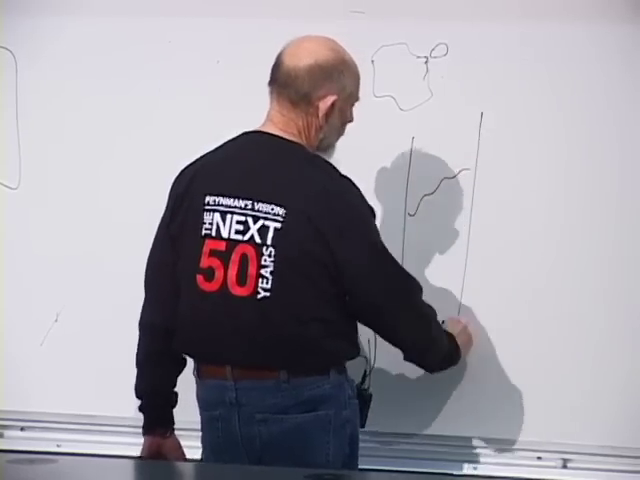
\includegraphics[width=0.72\textwidth]{lecture_06_figure_03.png}
\caption{Le schéma d’échange complété au tableau : un facteur de couplage intervient à l’émission, puis de nouveau à l’absorption.}
\lectureframe{00:11:30.000}
\end{figure}

Dans la version de la théorie des cordes, le graviton remplace le photon et \(g_s\) remplace la charge électrique. Un facteur accompagne l’émission et un autre l’absorption ; l’intensité de l’interaction gravitationnelle est donc proportionnelle à \(g_s^2\).

À grande distance, la même interaction doit reproduire la loi de force de Newton,
\begin{equation}
F_{\mathrm{grav}}\sim G_N\frac{M_1M_2}{r^2}.
\end{equation}
Les masses et la dépendance en l’inverse du carré décrivent les sources et la propagation ; ce qui nous importe ici, c’est le couplage qui les multiplie.

\begin{figure}[htbp]
\centering
\begin{tikzpicture}[x=1cm,y=1cm]
  \node[font=\small\bfseries] at (1.8,3.55) {electromagnetism};
  \draw[line width=0.8pt] (0,0) -- (0,3);
  \draw[line width=0.8pt] (3.6,0) -- (3.6,3);
  \draw[line width=0.8pt] plot[smooth] coordinates {(0,1.5) (0.45,1.72) (0.9,1.28) (1.35,1.72) (1.8,1.28) (2.25,1.72) (2.7,1.28) (3.15,1.72) (3.6,1.5)};
  \node[below] at (0,1.42) {\(e\)};
  \node[below] at (3.6,1.42) {\(e\)};
  \node[font=\small] at (1.8,0.25) {exchange strength \(\propto e^2\)};
  \node[font=\small\bfseries] at (7.2,3.55) {string gravity};
  \draw[line width=0.8pt,rounded corners=6pt] (5.4,0) -- (5.2,0.7) -- (5.5,1.5) -- (5.25,2.3) -- (5.4,3);
  \draw[line width=0.8pt,rounded corners=6pt] (9,0) -- (9.2,0.7) -- (8.9,1.5) -- (9.15,2.3) -- (9,3);
  \draw[line width=0.8pt] plot[smooth] coordinates {(5.5,1.5) (5.95,1.72) (6.4,1.28) (6.85,1.72) (7.3,1.28) (7.75,1.72) (8.2,1.28) (8.65,1.72) (8.9,1.5)};
  \node[below] at (5.5,1.42) {\(g_s\)};
  \node[below] at (8.9,1.42) {\(g_s\)};
  \node[font=\small] at (7.2,0.25) {exchange strength \(\propto g_s^2\)};
\end{tikzpicture}
\caption{L’analogie pour le décompte des couplages. Chaque extrémité du quantum échangé contribue un facteur d’interaction.}
\end{figure}

Cette observation permet de déterminer presque entièrement la constante de Newton. Le couplage \(g_s\) est sans dimension, tandis qu’en quatre dimensions \(G_N\) a les dimensions du carré d’une longueur. La longueur microscopique disponible est \(\ell_s\) ; on a donc
\begin{equation}
G_N\sim g_s^2\ell_s^2.
\label{eq:l06-newton-string}
\end{equation}
En combinant cela avec l’équation~\eqref{eq:l06-planck-area}, on obtient
\begin{equation}
\ell_p\sim g_s\ell_s.
\label{eq:l06-planck-string}
\end{equation}

\begin{figure}[htbp]
\centering
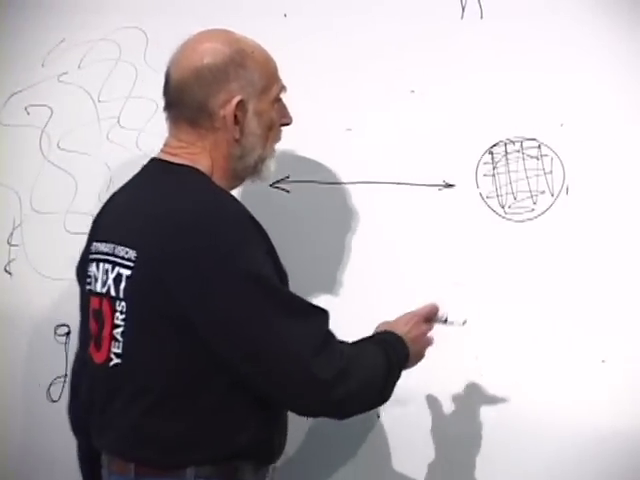
\includegraphics[width=0.72\textwidth]{lecture_06_figure_04.png}
\caption{Les relations fondamentales conservées au tableau : \(\ell_p^2=G_N\) et \(\ell_p\sim g_s\ell_s\).}
\lectureframe{00:15:45.000}
\end{figure}

L’équation~\eqref{eq:l06-newton-string} est la relation simplifiée utilisée tout au long de ce cours.\editorialnote{Dans une théorie des cordes compactifiée, la constante de Newton effective en quatre dimensions dépend également du volume de compactification et de conventions d’ordre unité. Le cours néglige ces éléments pour isoler le comportement d’échelle de la correspondance.}

\begin{classroomqa}
\audiencequestion{Le couplage \(g_s\) est-il supérieur ou inférieur à un, et quelle longueur est la plus grande ?\lecturetimestamp{00:16:00}}
\lecturerresponse{Nous travaillons à faible couplage, \(g_s<1\). Alors, d’après \(\ell_p\sim g_s\ell_s\), la longueur de corde est supérieure à la longueur de Planck. Le fort couplage exige une autre description, dont nous n’avons pas besoin ici.}
\end{classroomqa}

\section{Le dénombrement des états du trou noir}

En omettant la constante de Boltzmann et les facteurs numériques, l’entropie de Bekenstein--Hawking s’écrit
\begin{equation}
S_{\mathrm{BH}}=\frac{A}{4G_N}sim\frac{A}{G_N}sim\frac{A}{\ell_p^2}.
\label{eq:l06-bh-area}
\end{equation}
Le facteur \(1/4\) est exact dans la formule semi-classique, mais il n’intervient pas dans cet argument d’échelle.

\begin{classroomqa}
\audiencequestion{L’indice ``BH'' signifie-t-il « trou noir » ou « Bekenstein--Hawking » ?\lecturetimestamp{00:16:51}}
\lecturerresponse{Pour notre propos, il peut nous rappeler les deux. L’essentiel est que l’entropie est l’aire de l’horizon mesurée en aires de Planck.}
\end{classroomqa}

Pour un trou noir de Schwarzschild en quatre dimensions,
\begin{equation}
R_s=2G_NM,
\qquad
A=4\pi R_s^2.
\end{equation}
En omettant \(2\) et \(4\pi\), comme le fait le cours,
\begin{align}
S_{\mathrm{BH}}
&\sim \frac{R_s^2}{G_N}
\sim \frac{(G_NM)^2}{G_N} \\
&\sim M^2G_N
\sim M^2\ell_p^2.
\label{eq:l06-bh-mass}
\end{align}
C’est cette forme que nous comparerons au dénombrement des états de corde.

\section{Une corde longue comme marche aléatoire}

Partons d’une petite corde et injectons-y de l’énergie. Une corde générique très excitée ne reste pas une boucle bien ordonnée. Elle devient un objet long et emmêlé, comme du fil de pêche après un moulinet sérieusement enchevêtré. Cet enchevêtrement a une entropie, car un très grand nombre de configurations se ressemblent à l’échelle macroscopique.

Pour les dénombrer, remplaçons l’espace par un réseau dont les arêtes ont une longueur \(\ell_s\). Les sites sont les sommets, les arêtes sont les segments et les carrés élémentaires sont les plaquettes. Une corde est représentée par une suite connexe d’arêtes. Ce modèle est volontairement grossier, mais le nombre exponentiel d’états qu’il donne reproduit le comportement d’échelle recherché.

\begin{figure}[htbp]
\centering
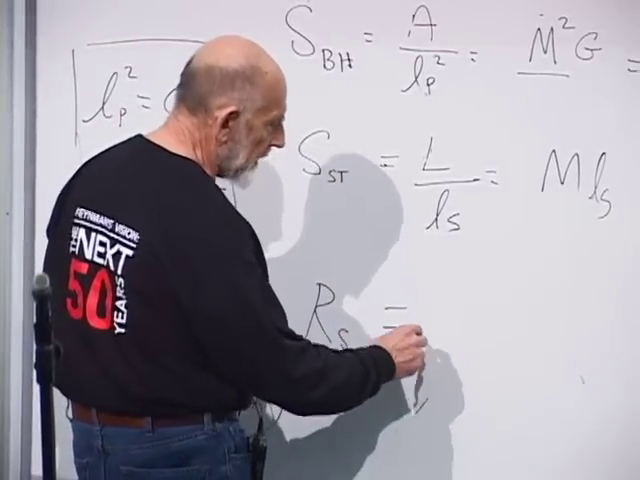
\includegraphics[width=0.72\textwidth]{lecture_06_figure_05.png}
\caption{Le modèle de réseau bidimensionnel. Le segment bleu représente un pas de la corde ; les quatre prolongements possibles sont comptés à chaque site.}
\lectureframe{00:23:50.000}
\end{figure}

\begin{classroomqa}
\audiencequestion{Combien de choix le modèle de marche simplifié offre-t-il à chaque pas ?\lecturetimestamp{00:22:43}}
\lecturerresponse{Quatre sur le réseau carré, puisque le retour immédiat en arrière est autorisé. En trois dimensions, il y en aurait six. Un autre réseau modifierait ce nombre ordinaire, mais le nombre de marches croîtrait toujours exponentiellement avec le nombre d’arêtes.}
\end{classroomqa}

Si la corde comporte \(n\) arêtes, le nombre d’états dans le modèle bidimensionnel est
\begin{equation}
\Omega_n\sim4^n.
\label{eq:l06-walk-count}
\end{equation}Il existe une marche rectiligne exceptionnelle, mais elle ne représente qu’un état parmi \(4^n\). Une marche typique se replie à plusieurs reprises et occupe une boule enchevêtrée. Pour un grand \(n\), presque toutes les configurations générées au hasard se ressemblent qualitativement.

L’entropie est le logarithme du nombre de configurations indiscernables à l’échelle macroscopique :
\begin{equation}
S_{\mathrm{st}}=\log\Omega_n\sim n\log4\sim n.
\label{eq:l06-string-entropy-n}
\end{equation}

\begin{classroomqa}
\audiencequestion{Pourquoi l’entropie est-elle proportionnelle à \(n\) plutôt qu’à \(4^n\) ?\lecturetimestamp{00:25:39}}
\lecturerresponse{L’entropie est le logarithme du nombre d’états. Ainsi, \(\log(4^n)=n\log4\), et le facteur \(\log4\) est une constante d’ordre unité que nous négligerons.}
\end{classroomqa}

Si \(L\) désigne la longueur de contour, obtenue en suivant la corde d’une extrémité à l’autre, alors
\begin{equation}
n=\frac{L}{\ell_s},
\qquad
S_{\mathrm{st}}\sim\frac{L}{\ell_s}.
\label{eq:l06-string-entropy-length}
\end{equation}
Ici, \(L\) ne désigne pas le diamètre de la boule enchevêtrée. C’est une distance bien plus grande, mesurée le long de la corde.

Passons ensuite de la longueur de contour à la masse. Avec \(c=\hbar=1\), la masse a les dimensions de l’inverse d’une longueur. Une arête de la taille d’une corde porte donc une masse de l’ordre de
\begin{equation}
m_{\mathrm{link}}\sim\frac{1}{\ell_s}.
\label{eq:l06-link-mass}
\end{equation}

\begin{classroomqa}
\audiencequestion{Pourquoi la masse d’une arête doit-elle être proportionnelle à \(1/\ell_s\) ?\lecturetimestamp{00:29:20}}
\lecturerresponse{Dans ces unités, la masse est l’inverse d’une longueur, et \(\ell_s\) est la seule longueur disponible. De façon équivalente, une tension de corde de l’ordre de \(1/\ell_s^2\), multipliée par la longueur d’une arête \(\ell_s\), donne le même résultat.}
\end{classroomqa}

La corde entière a alors
\begin{equation}
M\sim n m_{\mathrm{link}}
\sim\frac{n}{\ell_s}
\sim\frac{L}{\ell_s^2},
\qquad
L\sim M\ell_s^2.
\label{eq:l06-string-mass}
\end{equation}En substituant dans l’équation~\eqref{eq:l06-string-entropy-length}, on obtient
\begin{equation}
S_{\mathrm{st}}\sim M\ell_s.
\label{eq:l06-string-entropy-mass}
\end{equation}Le modèle de marche sur réseau néglige les contraintes de la surface d’univers et les coefficients numériques, mais la croissance exponentielle du spectre d’une corde très excitée donne le même comportement dominant.\editorialnote{La construction par marche aléatoire est un aide-mémoire pour la densité des états de corde à grand niveau d’excitation, et non une discrétisation littérale d’une corde fondamentale.}

\section{Le décalage qui amorce l’argument}

Nous avons maintenant les deux résultats :
\begin{equation}
S_{\mathrm{BH}}\sim M^2\ell_p^2,
\qquad
S_{\mathrm{st}}\sim M\ell_s.
\label{eq:l06-two-entropies}
\end{equation}Ils se ressemblent, mais ne sont pas égaux à masse fixée et pour un couplage quelconque. L’expression de l’entropie du trou noir est quadratique en \(M\) ; celle de la corde est linéaire. On ne peut pas simplement déclarer qu’une corde chaude est un trou noir sans expliquer comment les deux régimes se rejoignent.

\begin{figure}[htbp]
\centering
\includegraphics[width=0.78\textwidth]{lecture_06_figure_06.png}
\caption{La comparaison bien visible au tableau : l’entropie du trou noir en haut, celle de la corde longue en bas, avec les relations de Planck--corde conservées à gauche.}
\lectureframe{00:33:20.000}
\end{figure}

C’est là que le cours s’est interrompu. Le suspense est utile : ce décalage ne réfute pas l’idée, il indique qu’il faut comparer le même état tout en faisant varier l’intensité de la gravitation.

\section{Faire varier le couplage}

Fixons \(\ell_s\) et imaginons que \(g_s\) puisse varier. Pour \(g_s=0\), les cordes ne se scindent ni ne fusionnent, et la gravitation disparaît puisque \(G_N\sim g_s^2\ell_s^2\). Un état suffisamment énergétique est alors une corde longue et faiblement interactive.

Augmentons lentement \(g_s\). Les interactions entre cordes deviennent possibles et, ce qui importe davantage dans l’argument présent, la gravitation se renforce.

\begin{classroomqa}
\audiencequestion{Quand \(g_s\) augmente, le premier effet est-il simplement que la corde se scinde en cordes plus courtes ?\lecturetimestamp{00:36:29}}
\lecturerresponse{Les scissions et les fusions deviennent possibles, mais fixons \(\ell_s\) et suivons l’état de forte entropie. L’effet central est que \(G_N\) augmente, si bien que l’auto-gravitation de la corde longue attire vers l’intérieur la boule enchevêtrée.}
\end{classroomqa}

L’objet se contracte et devient plus dense. Son énergie potentielle gravitationnelle est négative ; la contraction abaisse donc son énergie totale et, par conséquent, sa masse.

\begin{classroomqa}
\audiencequestion{L’énergie augmente-t-elle ou diminue-t-elle lorsque l’auto-gravitation rapproche les parties de la corde ?\lecturetimestamp{00:37:48}}
\lecturerresponse{Elle diminue. L’énergie de liaison devient plus négative. La masse peut varier au cours de cette évolution, même si nous continuons à suivre le même état.}
\end{classroomqa}

À terme, la taille de l’objet devient comparable à son rayon de Schwarzschild. Au-delà de ce point, la description en termes de trou noir devient naturelle. Une excitation initiale plus importante atteint cette condition à un couplage plus faible, car un objet plus massif nécessite moins d’intensité gravitationnelle pour former un horizon.

\begin{figure}[htbp]
\centering
\resizebox{0.95\linewidth}{!}{%
\begin{tikzpicture}[x=1cm,y=1cm,>=Latex]
  \draw[->,line width=0.9pt] (0,0) -- (11,0) node[right] {increasing \(g_s\)};
  \node[draw,rounded corners,align=center,minimum width=2.6cm,minimum height=1.15cm] at (1.8,1.5) {long excited string\\weak self-gravity};
  \node[draw,rounded corners,align=center,minimum width=2.6cm,minimum height=1.15cm] at (5.5,1.5) {correspondence point\\\(R_s\sim\ell_s\)};
  \node[draw,circle,align=center,minimum size=1.8cm] at (9.3,1.5) {black\\hole};
  \draw[->,line width=0.8pt] (3.15,1.5) -- (4.1,1.5) node[midway,above,font=\small] {contracts};
  \draw[->,line width=0.8pt] (6.9,1.5) -- (8.25,1.5);
  \node[font=\small,align=center] at (5.5,-0.65) {same family of states followed slowly;\\binding energy and mass may change};
\end{tikzpicture}
}
\caption{Le parcours de correspondance à \(\ell_s\) fixée. Inverser la flèche ramène l’état de trou noir à un état de corde longue.}
\end{figure}

\begin{classroomqa}
\audiencequestion{Faut-il imaginer \(g_s\) entre zéro et un ?\lecturetimestamp{00:40:18}}
\lecturerresponse{Oui. L’argument reste dans le régime de faible couplage. Si \(g_s\) est très petit, l’état doit être d’autant plus massif pour devenir un trou noir. Nous n’avons pas besoin d’entrer dans le régime \(g_s>1\), mal contrôlé.}
\end{classroomqa}

Dans cette expérience de pensée, la variation lente est réversible.

\begin{classroomqa}
\audiencequestion{Si l’on réduit de nouveau le couplage jusqu’à ce que la gravitation ne puisse plus maintenir le trou noir, en quoi se transforme-t-il ?\lecturetimestamp{00:41:37}}
\lecturerresponse{En une corde longue. Lorsque la gravitation s’annule, tout ce qui intervient dans cette construction doit être décrit en termes d’états de corde. En faisant varier le couplage dans un sens, on passe de la corde au trou noir ; dans l’autre, du trou noir à la corde.}
\end{classroomqa}

À énergie totale et volume fixés, la configuration dominante de forte entropie est essentiellement une corde longue, plutôt qu’un très grand nombre de cordes courtes. Ce résultat n’est pas démontré ici. Il découle de la mécanique statistique des cordes près du régime de Hagedorn et nous y reviendrons.

\section{Ce que voit un observateur extérieur}

Où se trouve la corde lorsque l’objet est décrit comme un trou noir ? Dans la description extérieure, elle ne disparaît pas brusquement. En temps de Schwarzschild, le franchissement apparent est repoussé à un temps arbitrairement lointain ; les degrés de liberté de corde sont donc représentés comme s’accumulant sur l’horizon ou à proximité.

\begin{figure}[htbp]
\centering
\includegraphics[width=0.72\textwidth]{lecture_06_figure_07.png}
\caption{Comparaison au tableau entre un horizon macroscopique, où la structure à l’échelle de la corde forme une mince couche floue, et un horizon plus petit dont le rayon approche l’échelle de la boucle.}
\lectureframe{00:45:30.000}
\end{figure}

Pour \(R_s\gg\ell_s\), le trou noir est macroscopique et la structure à l’échelle de la corde ne forme qu’une mince couche par rapport au rayon de l’horizon. À mesure que le rayon diminue vers \(\ell_s\), la distinction entre un trou noir lisse et une corde étendue perd son sens. Il s’agit d’une description depuis l’extérieur, en termes d’horizon étiré ; il ne faut pas la confondre avec l’affirmation indépendante des coordonnées selon laquelle la matière en chute ne franchirait jamais un horizon régulier.\editorialnote{Le cours utilise la description extérieure familière dans le cadre de la complémentarité des trous noirs. L’expression ``sur l’horizon''désigne les degrés de liberté résolus dans la description extérieure ; elle ne constitue pas une dérivation distincte de leur position covariante.}

Le passage d’un régime à l’autre se produit lorsque
\begin{equation}
R_s\sim\ell_s.
\label{eq:l06-correspondence-radius}
\end{equation}En dessous de l’échelle de corde, la géométrie de Schwarzschild ne peut pas résoudre la structure censée la soutenir. Les boucles fluctuent hors de l’horizon éventuel, et il vaut mieux appeler corde l’état obtenu.

\section{Le point de correspondance}

Utilisons \(R_s\sim G_NM\) dans l’équation~\eqref{eq:l06-correspondence-radius} :
\begin{equation}
G_NM\sim\ell_s.
\end{equation}Substituons ensuite \(G_N\sim g_s^2\ell_s^2\) :
\begin{equation}
M g_s^2\ell_s^2\sim\ell_s,
\qquad
M g_s^2\ell_s\sim1.
\label{eq:l06-correspondence-condition}
\end{equation}

\begin{figure}[htbp]
\centering
\includegraphics[width=0.72\textwidth]{lecture_06_figure_08.png}
\caption{Le calcul complet de la transition au tableau : \(R_s\sim\ell_s\) mène à la condition sans dimension encadrée \(Mg_s^2\ell_s\sim1\).}
\lectureframe{00:49:50.000}
\end{figure}

Un membre de l’auditoire a remarqué ce que cette condition annonce. Au point de correspondance,
\begin{align}
S_{\mathrm{BH}}
&\sim M^2\ell_p^2
\sim M^2g_s^2\ell_s^2 \\
&=(M\ell_s)(Mg_s^2\ell_s)
\sim M\ell_s
\sim S_{\mathrm{st}}.
\label{eq:l06-entropy-preview}
\end{align}

\begin{classroomqa}
\audiencequestion{Les équations impliquent-elles déjà que les entropies du trou noir et de la corde deviennent égales ?\lecturetimestamp{00:50:18}}
\lecturerresponse{Oui. C’est exactement là que mène le calcul. Les éléments nécessaires ont été inscrits au tableau, mais le cours en reporte l’assemblage complet afin de revoir soigneusement le raisonnement de la correspondance.}
\end{classroomqa}

L’équation~\eqref{eq:l06-entropy-preview} donne en une ligne l’aperçu algébrique implicite dans l’échange. Elle établit le comportement d’échelle, mais pas le coefficient exact \(1/4\). Pour obtenir une égalité microscopique exacte, il faut des trous noirs mieux contrôlés et des constructions de cordes plus détaillées.\editorialnote{Le cours s’arrête avant de présenter l’équation~\eqref{eq:l06-entropy-preview} comme une dérivation complète. Elle est écrite ici parce que l’auditoire énonce explicitement l’égalité et que toutes les relations nécessaires ont déjà été introduites.}

\section{Pourquoi l’entropie se conserve au cours du passage}

Supposons qu’un paramètre de contrôle, tel qu’un champ magnétique ou \(g_s\), varie suffisamment lentement tandis que le système est isolé et que l’évolution est réversible. L’énergie, la taille et l’énergie de liaison peuvent changer, mais l’entropie est conservée :
\begin{equation}
\Delta S=0.
\label{eq:l06-adiabatic-entropy}
\end{equation}Le cours relie cela à la conservation de l’information. L’entropie mesure l’information masquée par une description à gros grains ; une variation lente et réversible du Hamiltonien réorganise les états sans effacer cette information.

\begin{classroomqa}
\audiencequestion{La conservation de l’entropie exige-t-elle que le parcours évite une transition de phase ?\lecturetimestamp{00:54:01}}
\lecturerresponse{Oui, il faut pouvoir suivre l’état de façon continue. Un système fini ne connaît pas de transition de phase thermodynamique strictement non analytique comme celle d’un système de volume infini ; si la variation est suffisamment lente, la correspondance peut être traitée comme un croisement continu.}
\end{classroomqa}

Le terme « adiabatique » est employé ici au sens plus fort de quasistatique et réversible. Un processus adiabatique mais irréversible peut produire de l’entropie ; la lenteur et la possibilité de suivre l’état sont essentielles.\editorialnote{L’énoncé thermodynamique \(\Delta S=0\) exige un parcours adiabatique réversible. En mécanique quantique, l’idée correspondante consiste à suivre le même ensemble d’états lorsque le paramètre varie, sans transitions incontrôlées entre niveaux.}

\begin{classroomqa}
\audiencequestion{Pourquoi une corde longue aurait-elle plus d’entropie que plusieurs cordes plus courtes de même masse totale ?\lecturetimestamp{00:54:44}}
\lecturerresponse{C’est contre-intuitif, mais le dénombrement explicite des états à haute énergie favorise une composante de corde longue dans un volume fixé. La démonstration est reportée ; pour l’argument présent, il nous suffit que le trou noir corresponde au secteur de cordes d’entropie maximale, plutôt qu’à un gaz dilué d’un très grand nombre de cordes courtes.}
\end{classroomqa}

La stratégie opératoire est donc la suivante :
\begin{enumerate}
\item Partir d’un trou noir de masse \(M_0\) et de couplage \(g_{s,0}\).
\item Diminuer lentement \(g_s\) tout en suivant la même famille d’états de forte entropie.
\item S’arrêter à \(R_s\sim\ell_s\), là où la description en termes de trou noir devient une description en termes de corde longue.
\item Dénombrer les états de corde à l’aide de \(S_{\mathrm{st}}\sim M\ell_s\).
\item Reporter cette entropie le long du parcours réversible jusqu’au trou noir initial.
\end{enumerate}

\begin{figure}[htbp]
\centering
\includegraphics[width=0.72\textwidth]{lecture_06_figure_09.png}
\caption{Le principe conservé au tableau pendant l’énoncé de la stratégie : une variation adiabatique de \(g_s\) ne modifie pas \(S\).}
\lectureframe{00:56:40.000}
\end{figure}

La théorie des cordes a permis d’obtenir des dénombrements d’entropie beaucoup plus précis pour les trous noirs chargés, en rotation, supersymétriques, presque extrémaux et de dimension supérieure. La discussion du trou noir neutre de Schwarzschild présentée ici est un argument de correspondance sommaire : elle établit la densité paramétrique des états et le passage physique d’un régime à l’autre, mais pas une dégénérescence protégée exacte.\editorialnote{L’accord exact est le plus solide pour les trous noirs particuliers dont le dénombrement des états reste protégé lorsque le couplage varie. Ce cours présente volontairement la version la plus simple, à l’ordre de grandeur près.}

\begin{classroomqa}
\audiencequestion{Lorsque la gravitation est coupée, l’état peut-il devenir deux cordes plutôt qu’exactement une ?\lecturetimestamp{00:58:25}}
\lecturerresponse{La probabilité d’obtenir un petit nombre de cordes longues est finie, et en utiliser deux au lieu d’une ne change pas le comportement dominant de l’entropie. Ce qui modifierait l’argument serait une fragmentation en un vaste gaz de cordes courtes ; le dénombrement statistique à haute énergie ne favorise pas cette issue.}
\end{classroomqa}

Le trou noir représente l’entropie maximale que l’on puisse concentrer dans une région ; lorsque la gravitation est supprimée, la corde longue est l’état correspondant de forte entropie. Ces deux descriptions sont désormais reliées, mais le calcul n’est pas encore développé avec précision. L’étape suivante consiste à reprendre soigneusement l’algèbre et à examiner jusqu’où l’on peut se fier à cette correspondance.

\chapter{Entropie des trous noirs, holographie et espace de de Sitter}

\lectureoverview{Nous achevons l’argument de correspondance amorcé au cours précédent. L’entropie d’une corde très excitée est proportionnelle à sa masse, tandis que celle d’un trou noir de Schwarzschild est proportionnelle à son aire. Ces deux formules ne se relient pas en identifiant un trou noir fortement gravitant à une corde libre, mais en faisant varier lentement le couplage des cordes jusqu’à ce que les deux descriptions se rejoignent. La loi en aire mène alors naturellement au principe holographique, et la dernière partie du cours introduit l’espace en expansion et la géométrie de de Sitter, dont nous étudierons l’horizon au prochain cours.}

\section{Retour au problème de dénombrement}

Il restait un point à régler dans le dénombrement des cordes longues. Si l’on répartit une longueur totale fixe entre plusieurs cordes, des cordes identiques de même longueur sont indiscernables. Leurs positions dans la boîte font néanmoins partie de l’état, et la boîte est choisie de façon à avoir à peu près la taille de la région occupée par la corde longue correspondante.

\begin{classroomqa}
\audiencequestion{Les cordes courtes sont-elles distinguables les unes des autres, et leurs positions comptent-elles ?\lecturetimestamp{00:00:37}}
\lecturerresponse{Des cordes aux propriétés identiques sont indiscernables, mais on dénombre leurs positions dans la boîte. La comparaison se fait à volume fixé, choisi pour correspondre à la région occupée par la corde longue.}
\end{classroomqa}

Cela réglé, nous pouvons énoncer l’objectif. Nous allons rassembler une courte liste d’équations et nous en servir pour obtenir la dépendance de l’entropie d’un trou noir. Aucun intégrale ni aucune somme infinie n’est nécessaire. La difficulté n’est pas algébrique : elle consiste à savoir quelles grandeurs peuvent être comparées et à quel stade du raisonnement.

\section{Unités naturelles et aire de Planck}

Posons
\begin{equation}
c=\hbar=1,
\label{eq:l07-natural-units}
\end{equation}
mais gardons explicite la constante de Newton. Il en découle d’abord que le temps et la longueur ont les mêmes unités. La relation pour les photons
\begin{equation}
E=\frac{\hbar c}{\lambda}
\end{equation}
et la relation masse-énergie \(E=mc^2\) impliquent alors
\begin{equation}
[M]=L^{-1}.
\label{eq:l07-mass-dimension}
\end{equation}
On peut donc exprimer une masse en inverse d’une longueur.

\begin{figure}[htbp]
\centering
\includegraphics[width=0.62\textwidth]{lecture_07_figure_02.png}
\caption{Convention des unités naturelles au début de l’argument dimensionnel. La formule de l’énergie est complétée par les équations ci-dessus.}
\lectureframe{00:03:27.900}
\end{figure}

Pour déterminer les unités de \(G_N\), utilisons l’accélération newtonienne à seule fin de tenir compte des dimensions :
\begin{equation}
a\sim\frac{G_NM}{R^2}.
\end{equation}
Comme \(T\) et \(L\) ont les mêmes unités, \([a]=L/T^2=L^{-1}\). Avec l’équation~\eqref{eq:l07-mass-dimension}, cela donne
\begin{equation}
[G_N]=L^2.
\end{equation}
Dans ces unités, la constante de Newton a les dimensions d’une aire. En définissant la longueur de Planck par
\begin{equation}
G_N=\ell_p^2,
\label{eq:l07-planck-area}
\end{equation}
on comprend aussitôt pourquoi \(A/G_N=A/\ell_p^2\) est sans dimension : elle mesure une aire en unités d’aire de Planck.

\section{Le couplage des cordes et l’intensité de la gravitation}

Il faut maintenant traduire la gravitation dans le langage des cordes. L’image utile est celle d’un processus d’échange. Lorsqu’une corde se croise elle-même, elle peut se scinder puis se rejoindre. Une petite boucle de corde fermée peut être émise par un objet et absorbée par un autre ; si cette excitation est un graviton, le processus véhicule la gravitation. Un facteur d’interaction intervient à l’émission, un autre à l’absorption : l’intensité de l’échange comporte donc \(g_s^2\).

Le couplage \(g_s\) est sans dimension. Plus précisément, c’est un couplage au niveau des amplitudes, tandis qu’une probabilité ou un taux apparaît à l’ordre \(g_s^2\).\editorialnote{Dans le cours, \(g_s\) est parfois appelé une probabilité, puis le propos est rectifié : il s’agit de la racine carrée d’une probabilité. Le couplage perturbatif intervient au niveau des amplitudes.} Comme \(G_N\) a les dimensions d’une aire, il manque encore une échelle de longueur. La longueur fondamentale des cordes \(\ell_s\), qui caractérise une oscillation élémentaire de corde, la fournit :
\begin{equation}
G_N\sim g_s^2\ell_s^2,
\qquad
\ell_p\sim g_s\ell_s.
\label{eq:l07-planck-string}
\end{equation}

\begin{figure}[htbp]
\centering
\includegraphics[width=0.72\textwidth]{lecture_07_figure_05.png}
\caption{Relation entre les couplages inscrite au tableau : \(G_N=\ell_p^2\) et \(g_s^2\ell_s^2\sim\ell_p^2\).}
\lectureframe{00:12:15.000}
\end{figure}

À faible couplage, \(g_s\ll1\), la longueur de Planck est très inférieure à la longueur des cordes. Diminuer \(g_s\) affaiblit la gravitation tout en laissant fixe l’échelle de longueur élémentaire des cordes.\editorialnote{Dans une théorie effective à quatre dimensions, les données de compactification et les conventions numériques interviennent également dans \(G_N\). Elles sont maintenues fixes et omises dans cet argument d’échelle.}

\section{Dénombrement d’une corde longue}

L’entropie dénombre les choix élémentaires nécessaires pour spécifier un état. Représentons une corde très excitée par une marche sur un réseau carré. À chaque sommet, le lien suivant peut pointer dans l’une de quatre directions. Décrire le choix élémentaire comme une décision à quatre possibilités ou comme deux décisions binaires ne change qu’une constante d’ordre unité. Ce qui importe, c’est le nombre de pas.

Si \(L\) est la longueur de contour de la corde et si chaque pas a pour longueur \(\ell_s\), il faut
\begin{equation}
N=\frac{L}{\ell_s}
\end{equation}
pas. Le nombre de marches croît exponentiellement, schématiquement comme \(\Omega_N\sim q^N\), où \(q\) est d’ordre unité ; on obtient donc
\begin{equation}
S_{\mathrm{str}}=\log\Omega_N\sim N\sim\frac{L}{\ell_s}.
\label{eq:l07-string-entropy-length}
\end{equation}

\begin{figure}[htbp]
\centering
\includegraphics[width=0.68\textwidth]{lecture_07_figure_03.png}

\vspace{0.7em}
\begin{tikzpicture}[scale=0.82]
  \draw[step=0.8cm,gray!45,thin] (0,0) grid (6.4,4.0);
  \draw[very thick,blue!60!black]
    (0.8,0.8)--(1.6,0.8)--(1.6,1.6)--(2.4,1.6)--(2.4,2.4)--
    (3.2,2.4)--(3.2,1.6)--(4.0,1.6)--(4.0,2.4)--(4.8,2.4)--
    (4.8,3.2)--(5.6,3.2);
  \draw[<->,thick] (0.8,-0.35)--(1.6,-0.35);
  \node[below] at (1.2,-0.35) {step \(\ell_s\)};
  \node[align=center] at (8.1,2.0) {\(N=L/\ell_s\) steps\\[0.3em]\(S_{\mathrm{str}}\sim N\)};
\end{tikzpicture}
\caption{Modèle sur réseau inscrit au tableau et interprétation épurée en termes de marche aléatoire. C’est la longueur de contour, et non le diamètre de la boule emmêlée, qui détermine le nombre de choix.}
\lectureframe{00:17:20.000}
\end{figure}

On dénombre la masse à partir des mêmes segments élémentaires. Un segment de longueur \(\ell_s\) a une échelle de masse de
\begin{equation}
m_{\mathrm{seg}}\sim\frac{1}{\ell_s}.
\end{equation}

\begin{classroomqa}
\audiencequestion{Attribue-t-on au segment élémentaire la longueur \(\ell_s\) ?\lecturetimestamp{00:18:56}}
\lecturerresponse{Oui. Sa longueur caractéristique est \(\ell_s\), donc, en unités naturelles, sa masse caractéristique est \(1/\ell_s\).}
\end{classroomqa}

En additionnant les masses des segments \(L/\ell_s\), on obtient
\begin{equation}
M\sim\frac{L}{\ell_s}\frac{1}{\ell_s}
=\frac{L}{\ell_s^2},
\qquad
L\sim M\ell_s^2.
\label{eq:l07-string-mass}
\end{equation}
Cette relation d’échelle condense les énergies cinétique et potentielle de la corde oscillante ; un traitement détaillé de mécanique statistique donne la même dépendance. En substituant dans l’équation~\eqref{eq:l07-string-entropy-length}, on obtient la formule pour la corde dont nous aurons besoin :
\begin{equation}
S_{\mathrm{str}}\sim M\ell_s.
\label{eq:l07-string-entropy-mass}
\end{equation}

\begin{figure}[htbp]
\centering
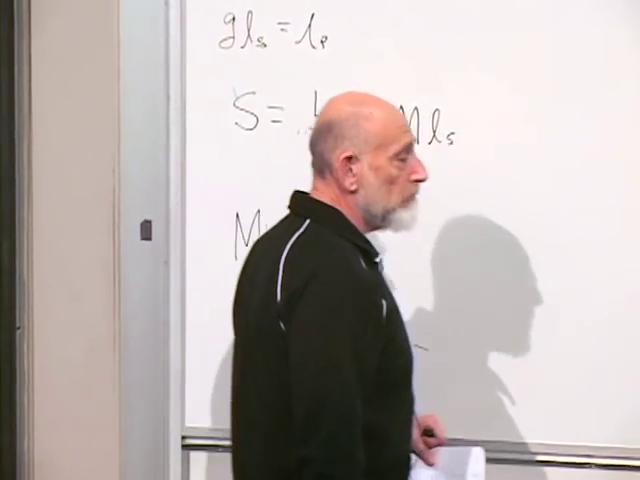
\includegraphics[width=0.66\textwidth]{lecture_07_figure_04.png}
\caption{La colonne consacrée aux cordes, assemblée avant la comparaison : \(\ell_p\sim g_s\ell_s\), \(S_{\mathrm{str}}\sim L/\ell_s\sim M\ell_s\) et \(M\sim L/\ell_s^2\).}
\lectureframe{00:21:57.800}
\end{figure}

\section{Pourquoi une corde libre n’est pas encore un trou noir}

Du côté gravitationnel, la formule semi-classique exacte est
\begin{equation}
S_{\mathrm{BH}}=\frac{A}{4G_N}.
\label{eq:l07-bh-exact}
\end{equation}

\begin{classroomqa}
\audiencequestion{Quel coefficient numérique faut-il mettre au dénominateur ?\lecturetimestamp{00:23:28}}
\lecturerresponse{Quatre. L’argument de correspondance retrouvera la dépendance d’échelle, mais il est trop grossier pour déterminer ce facteur exact.}
\end{classroomqa}

Pour un trou noir de Schwarzschild à quatre dimensions,
\begin{equation}
R_s=2G_NM,
\qquad
A=4\pi R_s^2.
\end{equation}
En négligeant les constantes numériques comme dans le cours,
\begin{align}
S_{\mathrm{BH}}
&\sim\frac{A}{G_N}
\sim\frac{(G_NM)^2}{G_N} \\
&\sim M^2G_N
\sim M^2\ell_p^2.
\label{eq:l07-bh-scaling}
\end{align}

\begin{figure}[htbp]
\centering
\includegraphics[width=0.72\textwidth]{lecture_07_figure_06.png}
\caption{Comparaison achevée au tableau : l’entropie de la corde est une longueur exprimée en unités de corde, tandis que celle du trou noir est une aire exprimée en unités de Planck.}
\lectureframe{00:25:35.000}
\end{figure}

La ressemblance entre les équations~\eqref{eq:l07-string-entropy-mass} et \eqref{eq:l07-bh-scaling} est suggestive, mais ce ne sont pas les mêmes formules. Il serait erroné de simplement qualifier de corde libre le trou noir initial et de faire la substitution. Le dénombrement d’une corde libre omet l’interaction attractive entre ses différentes parties, précisément celle qui compacte la corde en trou noir et abaisse son énergie totale par une énergie de liaison négative.

L’exemple d’une étoile rend l’erreur familière. Un gaz chaud de masse stellaire placé dans une boîte trop grande ne constitue pas un modèle d’étoile, même à la même température. L’auto-gravitation modifie la taille d’équilibre et la relation entre énergie et entropie. Suivre chacune des auto-interactions d’une corde longue serait difficile ; nous allons donc éviter de le faire.

\begin{classroomqa}
\audiencequestion{Si une petite boucle quitte une corde longue, son entropie diminue. L’échange de gravitons réduit-il donc l’entropie du système gravitant ?\lecturetimestamp{00:28:48}}
\lecturerresponse{Pas dans le processus d’échange à l’équilibre considéré ici. Des excitations virtuelles sont émises et absorbées dans les deux sens ; le schéma ne représente pas la perte littérale d’un fragment permanent de corde. Il sert uniquement, pour l’instant, à établir les deux facteurs de couplage et donc la dépendance en \(g_s^2\).}
\end{classroomqa}

\section{Le jeu de correspondance adiabatique}

Partons plutôt d’un régime où la gravitation est négligeable. Lorsque \(g_s\to0\), les cordes se croisent sans se scinder ni se rejoindre, et l’attraction gravitationnelle propre disparaît. Augmentons \(g_s\) en gardant \(\ell_s\) fixe : la gravitation se renforce, une corde très excitée se contracte et finit par devenir un trou noir. Si l’on inverse lentement le réglage, le trou noir doit redevenir un état de corde. Il peut se transformer en un petit nombre de cordes longues, mais le dénombrement à haute énergie du cours précédent indique que le secteur dominant contient une corde longue plutôt qu’un gaz immense de cordes courtes.

\begin{classroomqa}
\audiencequestion{Que maintient-on fixe pendant la variation du couplage ?\lecturetimestamp{00:32:19}}
\lecturerresponse{La longueur des cordes \(\ell_s\), et donc l’échelle de masse élémentaire des cordes \(1/\ell_s\), restent fixes. Le réglage modifie \(g_s\) et, par conséquent, \(G_N\sim g_s^2\ell_s^2\).}
\end{classroomqa}

La variation doit être lente, isolée et réversible. Dans ces conditions, l’entropie est un invariant adiabatique :
\begin{equation}
\Delta S=0.
\label{eq:l07-adiabatic}
\end{equation}
La lenteur ne suffit pas si des transitions dissipatives ou incontrôlées se produisent. Ici, ``adiabatique'' signifie que l’on peut suivre continûment une même famille d’états.\editorialnote{C’est le sens thermodynamique réversible du terme adiabatique. Un processus irréversible peut être adiabatique au sens d’une absence d’échange de chaleur et tout de même produire de l’entropie.}

Soit un trou noir cible de masse \(M_0\) et de couplage \(g_{s,0}\). Avant d’utiliser la formule de l’aire que nous cherchons à expliquer, l’analyse dimensionnelle indique seulement que l’entropie d’un trou noir neutre et non rotatif est une fonction de la combinaison sans dimension
\begin{equation}
S_{\mathrm{BH}}=f(M\ell_p)
=f(Mg_s\ell_s).
\label{eq:l07-entropy-function}
\end{equation}
À \(\ell_s\) fixé, un chemin isentropique conserve donc
\begin{equation}
Mg_s=M_0g_{s,0}
\label{eq:l07-adiabat}
\end{equation}
à condition de suivre la même branche d’états.

Quand \(g_s\) diminue, l’énergie de liaison négative est éliminée ; la masse \(M\) augmente donc le long de ce chemin. La configuration de corde sous-jacente est également moins fortement liée et s’étend. En revanche, le rayon de Schwarzschild formel évolue comme \(R_s\sim Mg_s^2\ell_s^2\sim g_s\ell_s\) sur l’adiabatique et diminue donc.\editorialnote{Dans la discussion orale, le terme ``grandit'' désigne l’objet libéré de sa liaison gravitationnelle. Il ne faut pas l’interpréter comme une augmentation du rayon de Schwarzschild le long de l’adiabatique déduite ici.}

\begin{classroomqa}
\audiencequestion{L’objet grandit-il ou rétrécit-il lorsque la gravitation s’affaiblit ?\lecturetimestamp{00:36:28}}
\lecturerresponse{Sa structure de corde est libérée et s’étend, tandis que sa masse augmente parce que l’énergie de liaison négative est éliminée. Le rayon attribué par la formule du trou noir diminue jusqu’à atteindre l’échelle des cordes, où cette description en trou noir cesse d’être utile.}
\end{classroomqa}

\section{Deux courbes et leur intersection}

Plaçons la masse en ordonnée et le couplage des cordes en abscisse. L’équation~\eqref{eq:l07-adiabat} est une hyperbole, \(M\propto g_s^{-1}\).

\begin{classroomqa}
\audiencequestion{Quel type de courbe correspond à un produit constant \(Mg_s\) ?\lecturetimestamp{00:44:08}}
\lecturerresponse{Une hyperbole. C’est l’adiabatique passant par le point cible \((g_{s,0},M_0)\).}
\end{classroomqa}

La seconde courbe marque le passage d’une description à l’autre. Un trou noir ne peut plus être décrit par une géométrie de Schwarzschild classique lorsque son rayon est inférieur à celui d’une oscillation élémentaire de corde. Nous estimons donc le point de correspondance par
\begin{equation}
R_s\sim\ell_s.
\label{eq:l07-correspondence-radius}
\end{equation}
En utilisant \(R_s\sim MG_N\) et l’équation~\eqref{eq:l07-planck-string}, on obtient
\begin{equation}
Mg_s^2\ell_s^2\sim\ell_s,
\qquad
Mg_s^2\sim\frac{1}{\ell_s}.
\label{eq:l07-transition-curve}
\end{equation}
La courbe de transition décroît donc comme \(M\propto g_s^{-2}\), plus rapidement que l’adiabatique.

\begin{figure}[htbp]
\centering
\includegraphics[width=0.70\textwidth]{lecture_07_figure_07.png}

\vspace{0.6em}
\begin{tikzpicture}[x=1cm,y=0.78cm]
  \draw[->] (0.4,0.4)--(7.0,0.4) node[right] {\(g_s\)};
  \draw[->] (0.4,0.4)--(0.4,6.5) node[above] {\(M\)};
  \draw[thick,black] plot[smooth] coordinates {(1.0,5.6) (1.5,4.0) (2.2,2.9) (3.2,2.1) (4.6,1.55) (6.3,1.2)};
  \draw[very thick,red!70!black] plot[smooth] coordinates {(1.25,6.0) (1.55,4.55) (2.0,3.15) (2.7,2.0) (3.8,1.25) (5.8,0.78)};
  \fill (2.05,3.1) circle (2pt) node[above right] {\((g_{s,*},M_*)\)};
  \node[black,rotate=-17] at (4.75,1.9) {\(Mg_s=M_0g_{s,0}\)};
  \node[red!70!black,rotate=-25] at (4.45,0.95) {\(Mg_s^2=1/\ell_s\)};
  \node at (5.75,3.5) {black hole};
  \node at (1.15,1.25) {string};
\end{tikzpicture}
\caption{Graphique du tableau et interprétation épurée. L’adiabatique noire coupe la courbe de correspondance rouge, plus pentue, au point où l’objet devient semblable à une corde.}
\lectureframe{00:49:35.000}
\end{figure}

À l’intersection \((M_*,g_{s,*})\), les deux équations sont
\begin{align}
M_*g_{s,*} &= M_0g_{s,0}, \\
M_*g_{s,*}^2 &\sim \frac{1}{\ell_s}.
\end{align}
Élevons la première équation au carré et divisons par la seconde :
\begin{equation}
M_*
\sim M_0^2g_{s,0}^2\ell_s.
\end{equation}
En multipliant par \(\ell_s\),
\begin{equation}
M_*\ell_s
\sim M_0^2g_{s,0}^2\ell_s^2
\sim M_0^2G_{N,0}.
\label{eq:l07-crossover-result}
\end{equation}

\begin{figure}[htbp]
\centering
\includegraphics[width=0.68\textwidth]{lecture_07_figure_08.png}
\caption{Calcul achevé du passage d’un régime à l’autre, y compris \(M_*\ell_s=M_0^2g_{s,0}^2\ell_s^2=M_0^2G_{N,0}\).}
\lectureframe{00:54:40.000}
\end{figure}

\begin{classroomqa}
\audiencequestion{En divisant les équations des deux courbes, \(\ell_s\) se retrouve-t-il au numérateur ou au dénominateur ?\lecturetimestamp{00:52:41}}
\lecturerresponse{Au numérateur. Diviser par \(1/\ell_s\) revient à multiplier par \(\ell_s\), d’où \(M_*\sim M_0^2g_{s,0}^2\ell_s\).}
\end{classroomqa}

Au point de transition, la formule pour la corde est valable, donc
\begin{equation}
S_*\sim M_*\ell_s.
\end{equation}
L’entropie est restée inchangée le long du chemin. En combinant ce résultat avec l’équation~\eqref{eq:l07-crossover-result}, on obtient l’entropie du trou noir cible initial :
\begin{equation}
S_{\mathrm{BH}}(M_0)
\sim M_0^2G_{N,0}
\sim M_0^2\ell_{p,0}^2.
\label{eq:l07-final-correspondence}
\end{equation}
C’est la dépendance en aire recherchée.

\section{Ce que la correspondance démontre et ne démontre pas}

Cette construction n’affirme pas que le trou noir initial, fortement gravitant, est une corde libre. Elle amène l’objet dans un régime où le dénombrement des cordes est fiable, en déduit l’entropie, puis reporte cette entropie le long d’un chemin réversible. La transition est un passage continu plutôt qu’une frontière de phase située précisément ; cette estimation ne peut donc déterminer le coefficient \(1/4\) de l’équation~\eqref{eq:l07-bh-exact}.

Le même raisonnement fonctionne néanmoins, à un facteur près, pour les trous noirs chargés, les objets noirs dans d’autres dimensions et les branes noires étendues. Des exemples plus symétriques et supersymétriques permettent des dénombrements protégés d’états, qui conservent une information exacte lorsque le couplage varie ; ces méthodes retrouvent les coefficients numériques, mais exigent un appareil mathématique dont l’argument conceptuel présenté ici n’a pas besoin.

Surtout, le calcul fournit une interprétation microscopique. L’entropie témoigne d’une structure cachée. La mécanique des fluides décrit la densité, la pression et l’écoulement sans faire intervenir les molécules ; l’entropie du fluide révèle l’existence de ces degrés de liberté microscopiques. De même, la relativité générale décrit un horizon sans montrer ses microétats. Le dénombrement des cordes montre qu’une théorie quantique cohérente de la gravitation peut contenir assez d’états pour rendre compte de l’entropie du trou noir.

\begin{classroomqa}
\audiencequestion{Qu’aurait donné \(S\sim M^3\ell_p^3\) à la place du résultat quadratique ?\lecturetimestamp{00:59:41}}
\lecturerresponse{On aurait obtenu une loi en volume. L’entropie de la matière ordinaire dans une pièce ou d’une tasse de café est proportionnelle au volume ; le résultat quadratique est particulier parce que, par l’intermédiaire de \(R_s\sim M\ell_p^2\), il est proportionnel à l’aire de l’horizon.}
\end{classroomqa}

Le résultat indique que l’entropie de Bekenstein--Hawking n’est pas une simple analogie thermodynamique formelle. Elle signale l’existence de degrés de liberté gravitationnels microscopiques, même si la dérivation élémentaire ne permet pas de les voir un à un.

\section{De l’entropie maximale à l’holographie}

Changeons maintenant de question. Au lieu de demander quelle est l’entropie d’un état donné, cherchons l’entropie maximale compatible avec une région.

Partons d’un modèle ordinaire de pièce sur réseau. Découpons le volume en cellules de taille \(V_{\mathrm{cell}}\), et attribuons à chacune une question binaire : occupée ou vide. Susskind donne à l’atome imaginaire le nom délibérément absurde de ``meatonium'', afin que les détails réalistes de la structure atomique ne détournent pas l’attention du dénombrement. Si
\begin{equation}
N=\frac{V}{V_{\mathrm{cell}}},
\end{equation}
alors le nombre de configurations et l’entropie maximale sont
\begin{equation}
\Omega=2^N,
\qquad
S_{\max}=\log\Omega=N\log2
\sim\frac{V}{V_{\mathrm{cell}}}.
\label{eq:l07-volume-count}
\end{equation}

\begin{figure}[htbp]
\centering
\includegraphics[width=0.68\textwidth]{lecture_07_figure_09.png}
\caption{La pièce découpée en cellules, chacune dans l’un de deux états. On dénombre une entropie maximale, et non l’entropie de la pièce bien rangée où se trouve la classe.}
\lectureframe{01:05:20.000}
\end{figure}

La pièce réelle est très loin de ce maximum. Un état explorant de manière chaotique tous ces choix dans les cellules serait extrêmement chaud. Ce que l’on retient du modèle jouet, c’est l’attente habituelle : le nombre de degrés de liberté indépendants, et donc l’entropie maximale, varie comme le volume.

La gravitation bouleverse cette attente. Considérons une région sphérique de frontière d’aire \(A\), d’entropie initiale \(S_{\mathrm{i}}\) et de masse \(M\), inférieure à la masse \(M_{\mathrm{BH}}\) du trou noir qui remplirait tout juste la sphère. Si \(M\) était plus grande, son horizon s’étendrait déjà au-delà de la frontière choisie.

Faisons maintenant entrer une coquille de masse \(M_{\mathrm{BH}}-M\). Sa composition n’a pas d’importance ; le cours envisage de la lumière, de la matière ordinaire ou même du fromage suisse. Organisons son effondrement. L’état final est un trou noir dont l’horizon remplit tout juste la région et dont l’entropie vaut
\begin{equation}
S_{\mathrm{f}}=\frac{A}{4G_N}.
\end{equation}
La deuxième loi impose
\begin{equation}
S_{\mathrm{i}}\le S_{\mathrm{f}}
=\frac{A}{4G_N}.
\label{eq:l07-holographic-bound}
\end{equation}

\begin{figure}[htbp]
\centering
\includegraphics[width=0.70\textwidth]{lecture_07_figure_10.png}

\vspace{0.5em}
\begin{tikzpicture}[scale=0.88]
  \draw[thick] (0,0) circle (1.35);
  \draw[very thick,red!70!black] (0,0) circle (2.05);
  \fill[gray!25] (0,0) circle (1.32);
  \node at (0,0) {\(M,S_{\mathrm{i}}\)};
  \draw[-{Latex[length=3mm]},thick,red!70!black] (3.5,0)--(2.15,0);
  \node[align=center,right] at (3.5,0) {incoming shell\\\(M_{\mathrm{BH}}-M\)};
  \node[below] at (0,-2.2) {final horizon area \(A\)};
\end{tikzpicture}
\caption{Construction avec une coquille. On fait entrer suffisamment de masse supplémentaire pour former un trou noir dont l’horizon remplit tout juste la région choisie.}
\lectureframe{01:13:30.000}
\end{figure}

Comme un trou noir de cette taille est un état admissible et qu’il sature l’inégalité, l’entropie maximale est
\begin{equation}
S_{\max}=\frac{A}{4G_N}.
\label{eq:l07-holographic-maximum}
\end{equation}
C’est le principe holographique sous forme de dénombrement : le nombre maximal de degrés de liberté indépendants dans une région gravitationnelle varie comme l’aire de sa frontière, soit approximativement un degré de liberté d’ordre unité par aire de Planck, plutôt que comme le nombre de volumes de Planck qu’elle contient.\editorialnote{L’argument de la coquille suppose que l’on peut enfermer la région et provoquer son effondrement de la manière décrite. Les espaces-temps plus généraux exigent des bornes covariantes sur l’entropie, mais l’argument sphérique saisit le principe utilisé dans le cours.}

L’écart est immense. L’intuition issue de la théorie locale des champs suggère que les choix effectués en différents points intérieurs devraient se combiner indépendamment et produire une loi en volume. La gravitation indique qu’un nombre suffisant de tels choix provoquerait l’effondrement de la région, et le trou noir fournit l’entropie admissible maximale. Le dénombrement par la frontière n’est donc pas une petite correction au dénombrement volumique : l’espace de Hilbert est organisé d’une manière différente.

\begin{classroomqa}
\audiencequestion{Que se passe-t-il dans un univers très vaste de densité à peu près uniforme ?\lecturetimestamp{01:15:48}}
\lecturerresponse{Cette question relève de la cosmologie plutôt que de la construction sphérique statique. Elle nous conduit à examiner les solutions en expansion des équations d’Einstein.}
\end{classroomqa}

\begin{classroomqa}
\audiencequestion{La borne en aire est-elle liée au principe d’incertitude ?\lecturetimestamp{01:16:03}}
\lecturerresponse{Le cours laisse cette question ouverte et passe ensuite à la cosmologie.}
\end{classroomqa}

\section{L’espace en expansion}

Nous ne dériverons pas ici les solutions cosmologiques à partir des équations d’Einstein ; nous les écrirons et apprendrons à les lire. Les tranches spatiales peuvent être fermées et à courbure positive, hyperboliques et à courbure négative, ou plates. Pour la discussion présente, considérons des tranches euclidiennes plates dans un espace-temps dépendant du temps.

\begin{classroomqa}
\audiencequestion{Quel est l’analogue de l’espace euclidien ordinaire pour l’espace-temps ?\lecturetimestamp{01:19:37}}
\lecturerresponse{L’espace de Minkowski. La cosmologie étudiée ici possède des tranches spatiales plates, mais son espace-temps n’est pas celui de Minkowski, car la métrique spatiale varie avec le temps.}
\end{classroomqa}

L’image familière du ballon décrit une surface fermée en expansion dans une dimension de moins. Susskind se souvient d’avoir tenté la démonstration avec un grand ballon marqué ; le marqueur a fragilisé le caoutchouc et provoqué un véritable éclatement. Cet incident met aussi en évidence un défaut conceptuel de l’analogie. Quand un ballon ordinaire se dilate, ses molécules de caoutchouc s’écartent et le matériau s’amincit jusqu’à se rompre. L’espace cosmologique ne voit pas ses lois locales se diluer. Pour préserver l’analogie, il faut imaginer que l’on ajoute sans cesse de nouvelles molécules de caoutchouc, afin que chaque petite région conserve les mêmes propriétés locales. Dans un modèle plat, remplaçons le ballon par une grande feuille que l’on étire uniformément et que l’on renouvelle de la même façon.

Mathématiquement, l’expansion figure dans la métrique :
\begin{equation}
\begin{aligned}
ds^2&=-dt^2+a(t)^2d\mathbf{x}^2,\\
d\mathbf{x}^2&=\delta_{ij}\,dx^i dx^j
=dx^2+dy^2+dz^2.
\end{aligned}
\label{eq:l07-frw-metric}
\end{equation}

\begin{figure}[htbp]
\centering
\includegraphics[width=0.72\textwidth]{lecture_07_figure_11.png}
\caption{Métrique d’expansion spatialement plate telle qu’elle est inscrite au tableau.}
\lectureframe{01:25:10.000}
\end{figure}

On appelle comobiles les points dont les coordonnées spatiales restent fixes. Si deux points comobiles ont une séparation coordonnée \(\Delta x\), leur distance propre à l’instant \(t\) vaut
\begin{equation}
D(t)=a(t)\Delta x.
\label{eq:l07-proper-distance}
\end{equation}
Leurs coordonnées ne varient pas, mais la distance métrique qui les sépare change. En dérivant à \(\Delta x\) fixe,
\begin{equation}
V=\dot D=\dot a\,\Delta x
=\frac{\dot a}{a}D.
\end{equation}
Définissons le paramètre de Hubble
\begin{equation}
H(t)=\frac{\dot a(t)}{a(t)}.
\label{eq:l07-hubble-parameter}
\end{equation}
Alors
\begin{equation}
V=H(t)D,
\label{eq:l07-hubble-law}
\end{equation}
C’est la loi de Hubble à un instant cosmique donné.

\begin{figure}[htbp]
\centering
\includegraphics[width=0.68\textwidth]{lecture_07_figure_12.png}
\caption{Loi de récession à temps égal inscrite au tableau : \(V=D\,\dot a/a\).}
\lectureframe{01:29:10.000}
\end{figure}

Le nom ``constante de Hubble'' peut induire en erreur. En général, \(H(t)\) varie avec le temps. Ce qui est constant dans l’espace, c’est le rapport \(V/D\) pour toute paire de points comobiles sur une même tranche de temps.

\begin{classroomqa}
\audiencequestion{Pour les galaxies lointaines, à quelle époque correspond le temps dans cette relation ? Nous les observons à une époque antérieure.\lecturetimestamp{01:31:10}}
\lecturerresponse{L’équation~\eqref{eq:l07-hubble-law} est une relation à temps égal. Une observation suit un rayon lumineux dirigé vers le passé et capte donc la galaxie lointaine à un instant antérieur ; la relation entre le décalage vers le rouge mesuré et la distance dépend donc de toute l’histoire le long du cône de lumière, et non d’une valeur instantanée de \(H\).}
\end{classroomqa}

\begin{figure}[htbp]
\centering
\includegraphics[width=0.66\textwidth]{lecture_07_figure_13.png}
\caption{Schéma d’espace-temps servant à distinguer une séparation à temps égal de ce qu’un observateur voit le long d’un rayon lumineux dirigé vers le passé.}
\lectureframe{01:33:20.000}
\end{figure}

\section{L’échelle de Hubble et l’expansion de de Sitter}

En unités \(c=1\), l’équation~\eqref{eq:l07-hubble-law} associe une vitesse de récession égale à 1 à la distance
\begin{equation}
D_H=\frac{1}{H}.
\label{eq:l07-hubble-radius}
\end{equation}
Des points comobiles plus éloignés peuvent avoir \(V>1\), voire \(V\gg1\), sans violer la relativité restreinte. Ils ne dépassent pas la vitesse de la lumière par rapport à un observateur local ; leur distance propre augmente parce que la géométrie intermédiaire se dilate.\editorialnote{Dans une cosmologie générale dépendant du temps, \(1/H\) est le rayon de Hubble, qui n’est pas automatiquement un horizon des événements. Dans le cas de de Sitter étudié ensuite, il devient l’échelle d’horizon constante.}

Dans de nombreux anciens modèles cosmologiques en décélération, \(H(t)\) diminue et \(1/H(t)\) augmente, si bien que des régions autrefois en récession supraluminique peuvent ensuite entrer en contact causal. Le tableau de l’avenir lointain décrit dans le cours tend plutôt vers une valeur positive constante \(H\). Alors \(1/H\) reste fixe, et l’équation d’expansion devient
\begin{equation}
\frac{\dot a}{a}=H,
\qquad
\dot a=Ha.
\label{eq:l07-constant-h}
\end{equation}

\begin{classroomqa}
\audiencequestion{Quelles sont les unités d’un paramètre de Hubble constant ?\lecturetimestamp{01:38:24}}
\lecturerresponse{L’inverse d’un temps. De manière équivalente, avec \(c=1\), c’est l’inverse d’une longueur. La grandeur \(H^{-1}\) fournit à la fois une échelle de temps d’expansion et une échelle de distance ; le cours donne comme exemple un ordre de grandeur d’environ quinze milliards d’années.}
\end{classroomqa}

La solution de l’équation~\eqref{eq:l07-constant-h} est
\begin{equation}
a(t)=a_0e^{Ht}.
\label{eq:l07-desitter-scale-factor}
\end{equation}

\begin{classroomqa}
\audiencequestion{Quelle fonction a un taux de variation proportionnel à elle-même ?\lecturetimestamp{01:39:04}}
\lecturerresponse{Une exponentielle. Le facteur d’échelle est donc \(a_0e^{Ht}\), tandis que le coefficient spatial \(a(t)^2\) de la métrique croît comme \(e^{2Ht}\).}
\end{classroomqa}

\begin{figure}[htbp]
\centering
\includegraphics[width=0.70\textwidth]{lecture_07_figure_14.png}
\caption{Équations à \(H\) constant et leur solution exponentielle inscrites au tableau.}
\lectureframe{01:39:30.000}
\end{figure}

Un espace-temps présentant cette expansion exponentielle est un espace de de Sitter. Son échelle de Hubble constante produit un horizon des événements à distance propre finie. La géométrie est, en un sens, le complément de celle d’un trou noir : un observateur demeure à l’intérieur d’un horizon cosmologique, tandis que des objets suffisamment éloignés s’éloignent et ne peuvent jamais lui envoyer de signaux qui le rattrapent. L’horizon d’un trou noir cache l’intérieur à un observateur extérieur ; l’horizon de de Sitter cache l’extérieur de la région accessible à l’observateur. Contrairement à un trou noir ordinaire qui s’évapore, la géométrie idéale de de Sitter est ici considérée comme persistante. La comparaison ne fait que commencer. Le prochain cours développera l’horizon, sa thermodynamique et les énigmes qu’il pose à la cosmologie.

\chapter{Énergie du vide et horizons de de Sitter}

\lectureoverview{L’énergie du vide diffère de la matière ordinaire : elle ne privilégie aucun référentiel inertiel et ne se dilue pas avec l’expansion de l’Univers. Dès que l’on tient compte de la gravité, ce zéro de l’énergie, apparemment anodin, modifie la géométrie de l’espace-temps. Nous établirons la loi de l’ère dominée par la matière \(a(t)\propto t^{2/3}\), la comparerons à celle de l’ère dominée par le vide \(a(t)\propto e^{Ht}\), puis réécrirons l’espace-temps de de Sitter en coordonnées conformes. Le diagramme causal qui en résulte révèle un horizon des événements, dépendant de l’observateur, situé à distance propre constante.}

\section{Fluctuations quantiques du vide}

Nous commencerons par la question qui motive tout ce cours. La théorie quantique des champs attribue une énergie à l’espace vide. Cela signifie-t-il que de véritables paires électron--positron émergent continuellement du néant ?

\begin{classroomqa}
\audiencequestion{La création et l’annihilation de paires électron--positron se produisent-elles réellement dans le vide, ou s’agit-il simplement d’un artifice comptable ?\lecturetimestamp{00:00:06}}
\lecturerresponse{Les paires virtuelles contribuent à l’énergie du vide, mais ce ne sont pas des particules ordinaires que l’on pourrait observer émergeant de l’espace vide. Ce sont des fluctuations de l’état fondamental quantique, qui ne persistent que dans les limites propres à un processus virtuel.}
\end{classroomqa}

L’oscillateur harmonique en fournit le modèle le plus simple. Classiquement, il peut rester immobile au minimum de son potentiel. En mécanique quantique, une position exactement égale au minimum et une quantité de mouvement exactement nulle sont incompatibles. L’état fondamental constitue un compromis entre les deux et conserve l’énergie du point zéro
\begin{equation}
E_0=\frac{1}{2}\hbar\omega.
\label{eq:l08-zero-point}
\end{equation}
C’est l’énergie minimale que l’oscillateur puisse avoir. Ce n’est pas un état excité et cela ne représente pas un flux de particules observables.

Un champ libre se décompose en modes normaux, dont chacun se comporte comme un oscillateur. Le champ électromagnétique dans une cavité en est un exemple familier. Chaque mode apporte un terme de la forme donnée à l’équation~\eqref{eq:l08-zero-point} ; les champs quantiques de l’électron, des quarks et d’autres particules apportent leurs propres fluctuations de l’état fondamental. La somme de ces contributions donne ce que nous appelons l’énergie du vide. L’écart notoire entre les estimations microscopiques naïves et l’échelle cosmologique observée est réel, mais ce n’est pas le sujet de ce cours.

\begin{classroomqa}
\audiencequestion{La différence d’environ \(120\) ordres de grandeur sera-t-elle abordée de nouveau ?\lecturetimestamp{00:02:59}}
\lecturerresponse{Pas ici. Le but est de comprendre les horizons cosmiques : comment les équations cosmologiques produisent une expansion accélérée et pourquoi celle-ci crée des horizons des événements.}
\end{classroomqa}

\begin{classroomqa}
\audiencequestion{La relation ultraviolet--infrarouge du cours précédent fait-elle partie de la discussion de ce soir ?\lecturetimestamp{00:03:59}}
\lecturerresponse{Nous y reviendrons peut-être plus tard, mais elle ne fait pas partie du raisonnement prévu. Le parcours immédiat va de l’énergie du vide à la cosmologie, puis aux horizons.}
\end{classroomqa}

\section{Pourquoi l’énergie du vide est invariante de Lorentz}

La question suivante semble élémentaire, mais elle met en évidence la propriété qui définit l’énergie du vide. Si l’espace vide possède une densité d’énergie positive, pourquoi ne se comporte-t-il pas comme un milieu optique et ne modifie-t-il pas la vitesse de la lumière ?

\begin{classroomqa}
\audiencequestion{Une densité d’énergie du vide positive devrait-elle avoir un effet réfractif et ralentir légèrement la lumière ?\lecturetimestamp{00:04:35}}
\lecturerresponse{La matière ordinaire peut produire cet effet parce qu’elle définit un référentiel de repos privilégié. L’énergie du vide est différente : elle ne sélectionne aucun référentiel de ce type, et tous les observateurs inertiels mesurent la même densité d’énergie du vide. Les mesures locales de la lumière donnent donc toujours la vitesse invariante \(c\).}
\end{classroomqa}

Il faut distinguer la symétrie des lois de celle d’un état particulier. Les lois de la physique peuvent être invariantes par translation, même si Stanford n’est pas Berkeley et si la Terre n’est pas l’espace interstellaire. La translation de \emph{l’ensemble} de la configuration physique laisse les lois inchangées ; la répartition réelle de la matière n’a pas besoin d’être identique en tout lieu. De même, des équations invariantes par rotation ne rendent pas cette salle de cours symétrique par rotation.

La même distinction s’applique aux transformations de Lorentz. Un gaz possède un référentiel de repos. Un observateur qui se déplace par rapport à lui voit des molécules en mouvement et mesure une densité d’énergie différente : l’état du gaz n’est donc pas invariant de Lorentz, même si les équations qui le régissent le sont. La matière ordinaire, les bains de rayonnement et les appareils de laboratoire brisent tous la symétrie en sélectionnant des mouvements ou des directions privilégiés.

L’énergie du vide est la forme exceptionnelle de matière qui ne fait rien de tel. Imaginons un détecteur qui mesure la densité d’énergie du vide. Au repos, il indique une certaine valeur \(\rho_{\rm vac}\). Accélérons le détecteur et répétons la mesure : le résultat ne change pas. En notation relativiste, cette propriété s’exprime par un tenseur énergie-impulsion proportionnel à la métrique,
\begin{equation}
T_{\mu\nu}^{\rm vac}=-\rho_{\rm vac}g_{\mu\nu},
\qquad
p_{\rm vac}=-\rho_{\rm vac}.
\label{eq:l08-vacuum-stress}
\end{equation}
\editorialnote{La relation entre pression et densité n’est pas déduite au tableau. Elle exprime de façon covariante les deux propriétés qui définissent l’énergie du vide dans ce cours : l’invariance de Lorentz et la constance de la densité pendant l’expansion.}

La précision « locale » est importante. Un rayon lumineux qui passe près d’un observateur est mesuré à l’aide d’horloges et de règles locales comme se déplaçant à \(c\). Demander la vitesse, par rapport à nous, d’un rayon lumineux lointain dans un espace en expansion nécessite de choisir des coordonnées et une méthode pour comparer des événements distants. Cette vitesse coordonnée n’a pas besoin d’être égale à \(c\), même si chaque observateur local mesure \(c\).

\begin{classroomqa}
\audiencequestion{Dans cette discussion, l’énergie du vide et la constante cosmologique sont-elles synonymes ?\lecturetimestamp{00:11:57}}
\lecturerresponse{Oui. Ce sont deux façons de placer le même terme dans les équations d’Einstein : on peut le décrire comme une constante cosmologique du côté géométrique, ou comme un tenseur énergie-impulsion du vide invariant de Lorentz du côté des sources.}
\end{classroomqa}

\section{Ce qui se dilue et ce qui ne se dilue pas}

Remplissons une vaste région de particules non relativistes de masse \(m\). À des échelles suffisamment grandes pour moyenner les galaxies et les amas, supposons la distribution homogène. Si un volume comobile contient \(N\) particules, sa densité de matière vaut
\begin{equation}
\rho_m=\frac{Nm}{V}.
\end{equation}
Lorsque chaque dimension linéaire double, le volume est multiplié par \(2^3=8\), tandis que \(N\) et \(m\) restent inchangés. La densité tombe donc au huitième de sa valeur initiale. La matière ordinaire se dilue parce que les mêmes particules occupent un volume physique plus grand.

Le rayonnement se dilue lui aussi, et plus rapidement. Sa densité numérique diminue avec le volume, tandis que la longueur d’onde de chaque photon est étirée et que son énergie subit un décalage vers le rouge. Nous noterons plus tard le résultat \(\rho_r\propto a^{-4}\), mais nous ne résoudrons pas ce soir la cosmologie dominée par le rayonnement.

L’énergie du vide fait exception :
\begin{equation}
\rho_{\rm vac}(t)=\text{constant}.
\label{eq:l08-rho-vac-constant}
\end{equation}
Elle ne s’agrège pas, ne sélectionne ni direction ni référentiel inertiel, et sa densité ne diminue pas avec l’expansion de l’espace. Si une boîte comobile grandit, l’énergie du vide qu’elle contient augmente en proportion de son volume.

\editorialnote{Une densité constante ne signifie pas que l’énergie totale du vide dans une boîte comobile en expansion reste constante. La conservation covariante du tenseur énergie-impulsion,
\(\dot\rho+3H(\rho+p)=0\), est satisfaite parce que l’énergie du vide a une pression négative \(p_{\rm vac}=-\rho_{\rm vac}\). Le terme de travail fournit exactement la variation de l’énergie totale du vide dans la boîte.}

\section{La gravité est sensible au zéro de l’énergie}

En physique de laboratoire sans gravitation, décaler toutes les énergies d’une même constante ne change généralement rien. Les spectres dépendent des différences d’énergie : entre un atome excité et un atome non excité, ou entre un état avec particule et un état sans particule. L’espace vide semble ne fournir aucun référentiel permettant de mesurer son énergie absolue.

La gravité change la question. La masse est de l’énergie, l’énergie est une source de gravitation, et l’énergie du vide gravite donc elle aussi. Une constante invisible dans une transition atomique peut courber l’espace-temps.

L’équation d’Einstein sépare la géométrie des sources :
\begin{equation}
G_{\mu\nu}=8\pi G_N T_{\mu\nu},
\label{eq:l08-einstein}
\end{equation}
dans un système d’unités où \(c=1\). Le tenseur d’Einstein \(G_{\mu\nu}\) est construit à partir de la métrique \(g_{\mu\nu}(x)\) et de ses dérivées. Le tenseur énergie-impulsion \(T_{\mu\nu}\) comprend la densité d’énergie, la densité de quantité de mouvement, la pression et les contraintes dues à la matière et aux champs non gravitationnels. L’énergie du vide figure du côté des sources, comme la matière ordinaire.\editorialnote{L’introduction orale associe brièvement \(8\pi/3\) à l’équation tensorielle. Le facteur \(1/3\) appartient à l’équation de Friedmann spatialement plate présentée ci-dessous, et non à l’équation~\eqref{eq:l08-einstein}.}

\begin{figure}[htbp]
\centering
\includegraphics[width=0.62\textwidth]{lecture_08_figure_02.png}
\caption{Le côté géométrique de l’équation d’Einstein, construit à partir de la métrique de l’espace-temps \(g_{\mu\nu}(x)\).}
\lectureframe{00:21:58.820}
\end{figure}

\section{Réduire la géométrie à un facteur d’échelle}

Choisissons maintenant la géométrie homogène en expansion la plus simple, avec des tranches spatiales plates :
\begin{equation}
ds^2=-dt^2+a(t)^2\,d\mathbf{x}^2,
\qquad
d\mathbf{x}^2=dx^2+dy^2+dz^2.
\label{eq:l08-frw-metric}
\end{equation}
Les coordonnées \(\mathbf{x}\) sont tracées sur une feuille de caoutchouc infinie. Elles peuvent rester immobiles, mais les distances physiques entre elles varient. Deux points comobiles séparés par \(\Delta\mathbf{x}\) sont à distance propre constante à \(t\) donnée
\begin{equation}
D(t)=a(t)\lvert\Delta\mathbf{x}\rvert.
\label{eq:l08-proper-distance}
\end{equation}
Ainsi, toute la dépendance temporelle de cette géométrie hautement symétrique est contenue dans une seule fonction, le facteur d’échelle \(a(t)\). Une valeur constante de \(a\) donne l’espace-temps plat de Minkowski après un changement d’échelle spatial. Un facteur \(a\) qui dépend du temps peut laisser chaque tranche spatiale plate tout en courbant l’espace-temps dans son ensemble.

\begin{classroomqa}
\audiencequestion{Pour des coordonnées \(x=7\) et \(x=13\), leur séparation en coordonnées est-elle \(4\) ?\lecturetimestamp{00:27:40}}
\lecturerresponse{Non. Elle vaut \(13-7=6\), et leur séparation physique vaut donc \(6a(t)\). Cette correction est utile : \(x\) repère la position comobile, tandis que la multiplication par \(a(t)\) donne la distance physique.}
\end{classroomqa}

Pour cette métrique et une densité d’énergie uniforme dans l’espace, une composante de l’équation d’Einstein devient l’équation de Friedmann spatialement plate,
\begin{equation}
\left(\frac{\dot a}{a}\right)^2
=\frac{8\pi G_N}{3}\rho(t).
\label{eq:l08-friedmann}
\end{equation}
Le rapport
\begin{equation}
H(t)\equiv\frac{\dot a(t)}{a(t)}
\label{eq:l08-hubble-definition}
\end{equation}
est le paramètre de Hubble. À ce stade, il est défini ainsi et peut dépendre du temps.

\begin{figure}[htbp]
\centering
\includegraphics[width=0.90\textwidth]{lecture_08_figure_03.png}
\caption{La métrique plate en expansion et l’équation de Friedmann, après rétablissement au tableau du facteur manquant \(1/a^2\).}
\lectureframe{00:30:30.000}
\end{figure}

\paragraph{L’interprétation en bilan énergétique.}
Dans ce bilan énergétique, l’équation~\eqref{eq:l08-friedmann} s’écrit schématiquement
\begin{equation}
-\frac{3}{8\pi G_N}H^2+\rho=0.
\label{eq:l08-energy-heuristic}
\end{equation}
L’énergie de la matière est positive, tandis que le degré de liberté gravitationnel représenté par le facteur d’échelle en expansion porte un terme cinétique négatif. Dans ce problème réduit, l’égalité entre énergie gravitationnelle négative plus énergie positive de la matière et zéro est un moyen mnémotechnique utile.

\editorialnote{L’équation~\eqref{eq:l08-energy-heuristic} est la contrainte hamiltonienne d’un modèle de minisuperspace hautement symétrique, et non un théorème indépendant des coordonnées selon lequel tout univers arbitraire posséderait une énergie totale globale conservée égale à zéro. Le cours l’utilise comme interprétation heuristique de la contrainte de Friedmann.}

\section{Expansion dominée par la matière}

Revenons à une boîte mathématique comobile de côté, en coordonnées, \(\Delta x=1\). Son côté physique vaut \(a(t)\), et son volume physique est donc \(a(t)^3\). Si elle contient \(N\) particules non relativistes de masse \(m\), alors
\begin{equation}
\rho_m(t)=\frac{Nm}{a(t)^3}
=\frac{\rho_0}{a(t)^3}.
\label{eq:l08-matter-density}
\end{equation}
Les particules elles-mêmes ne se dilatent pas ; c’est leur séparation moyenne qui augmente.

\begin{figure}[htbp]
\centering
\includegraphics[width=0.84\textwidth]{lecture_08_figure_04.png}
\caption{La métrique et l’équation de Friedmann au fil de la construction du raisonnement sur la boîte comobile.}
\lectureframe{00:36:07.940}
\end{figure}

En substituant dans l’équation~\eqref{eq:l08-friedmann}, on obtient
\begin{equation}
\left(\frac{\dot a}{a}\right)^2
=\frac{8\pi G_N\rho_0}{3a^3}.
\end{equation}
Posons \(K=8\pi G_N\rho_0/3\) et choisissons la branche en expansion :
\begin{align}
\dot a^2&=\frac{K}{a},\\
\dot a&=\sqrt{K}\,a^{-1/2},\\
a^{1/2}\,da&=\sqrt{K}\,dt.
\label{eq:l08-matter-separated}
\end{align}

\begin{classroomqa}
\audiencequestion{Comment résoudre l’équation après séparation des variables ?\lecturetimestamp{00:38:15}}
\lecturerresponse{Intégrons les deux membres. L’intégrale de \(a^{1/2}\,da\) est \(\frac{2}{3}a^{3/2}\), et non \(\frac{3}{2}a^{3/2}\) ; \(\frac{3}{2}\) est la nouvelle puissance, tandis que \(\frac{2}{3}\) est le coefficient.}
\end{classroomqa}

On obtient donc
\begin{equation}
\frac{2}{3}a^{3/2}
=\sqrt{K}\,(t-t_B),
\end{equation}
où \(t_B\) est une constante d’intégration qui fixe l’origine du temps choisie. À un facteur de normalisation près et à un décalage temporel près,
\begin{equation}
a(t)\propto (t-t_B)^{2/3}.
\label{eq:l08-matter-solution}
\end{equation}

\begin{figure}[htbp]
\centering
\includegraphics[width=0.86\textwidth]{lecture_08_figure_05.png}
\caption{Substitution de la densité de matière et séparation des variables conduisant à \(a^{1/2}da\propto dt\).}
\lectureframe{00:38:30.000}
\end{figure}

La courbe \(t^{2/3}\) croît moins vite qu’une droite. Sa pente diminue : l’expansion d’un univers dominé par la matière est donc décélérée. Dans le langage newtonien employé dans le cours, les particules ont commencé par s’éloigner les unes des autres et leur attraction gravitationnelle mutuelle réduit continuellement leur vitesse d’éloignement.

\begin{figure}[htbp]
\centering
\includegraphics[width=0.86\textwidth]{lecture_08_figure_06.png}
\caption{Comparaison au tableau entre une expansion linéaire et la loi de l’ère dominée par la matière, concave vers le bas, \(a(t)\propto t^{2/3}\).}
\lectureframe{00:40:00.000}
\end{figure}

À titre de repère, un bain de rayonnement vérifie
\begin{equation}
\rho_r\propto a^{-4},
\end{equation}
plutôt que \(a^{-3}\) : la dilution liée au volume apporte trois puissances et le décalage cosmologique vers le rouge en apporte une quatrième. Le facteur d’échelle correspondant peut également se calculer, mais le cours laisse volontairement cet exercice de côté.

\section{Expansion dominée par le vide}

Ne plaçons maintenant que l’énergie du vide du côté droit de l’équation de Friedmann. Puisque \(\rho_{\rm vac}\) est constante,
\begin{equation}
\left(\frac{\dot a}{a}\right)^2
=\frac{8\pi G_N}{3}\rho_{\rm vac}
\equiv H^2.
\label{eq:l08-de-sitter-friedmann}
\end{equation}
Il faut distinguer deux usages de \(H\). L’équation~\eqref{eq:l08-hubble-definition} définit la quantité, éventuellement dépendante du temps, \(\dot a/a\). L’équation~\eqref{eq:l08-de-sitter-friedmann} indique que, dans un univers composé uniquement d’énergie du vide, sa valeur est la constante
\begin{equation}
H=\sqrt{\frac{8\pi G_N\rho_{\rm vac}}{3}}.
\end{equation}
En prenant la branche en expansion, on obtient
\begin{equation}
\dot a=Ha,
\end{equation}
et donc
\begin{equation}
a(t)=C e^{Ht}.
\label{eq:l08-exponential-solution}
\end{equation}
La constante d’intégration \(C\) fixe la normalisation arbitraire des coordonnées comobiles. Une croissance proportionnelle à la valeur actuelle de \(a\) est une croissance exponentielle.

\begin{figure}[htbp]
\centering
\includegraphics[width=0.88\textwidth]{lecture_08_figure_07.png}
\caption{L’équation de l’expansion dominée par le vide \((\dot a/a)^2=H^2\), sa forme du premier ordre \(\dot a=Ha\) et la solution exponentielle.}
\lectureframe{00:47:45.000}
\end{figure}

La loi de Hubble pour des objets comobiles s’écrit
\begin{equation}
v_{\rm rec}=HD.
\label{eq:l08-hubble-law}
\end{equation}
Dans ce cas précis de de Sitter, la distance propre à laquelle la vitesse de récession est égale à \(c\) est constante :
\begin{equation}
D_H=\frac{c}{H},
\label{eq:l08-hubble-radius}
\end{equation}
ou \(D_H=H^{-1}\) dans le système d’unités \(c=1\) utilisé au tableau. Cette échelle fixe réapparaîtra géométriquement comme le rayon de l’horizon des événements de de Sitter.\editorialnote{Dans une cosmologie quelconque où le facteur d’échelle dépend du temps, le rayon de Hubble n’est pas automatiquement un horizon des événements. L’identification fonctionne ici parce que \(H\) est constant dans l’espace exact de de Sitter.}

Le cours propose une expérience de pensée avec un détecteur d’énergie du vide. Plaçons deux corps d’épreuve très légers loin de toute autre source, initialement au repos par rapport au flot comobile, et rendons leur attraction mutuelle négligeable. Leur séparation suit l’expansion exponentielle. L’effet est beaucoup trop faible pour être détecté par un appareil terrestre, mais les distances cosmiques et le temps rétrospectif le rendent observable.

\section{De la domination de la matière à celle du vide}

Le modèle cosmologique réel envisagé dans le cours comprend les deux termes :
\begin{equation}
H(t)^2
=\frac{8\pi G_N}{3}
\left(\frac{\rho_0}{a(t)^3}+\rho_{\rm vac}\right).
\label{eq:l08-mixed-friedmann}
\end{equation}
Pour de petites valeurs de \(a\), le terme de matière domine parce que \(a^{-3}\) est grand, et la solution ressemble à \(t^{2/3}\). À mesure que l’Univers grandit, la matière se dilue tandis que l’énergie du vide reste constante. Le terme constant finit par l’emporter et le facteur d’échelle se courbe vers le haut, en direction de \(e^{Ht}\).

\begin{figure}[htbp]
\centering
\includegraphics[width=0.87\textwidth]{lecture_08_figure_08.png}
\caption{La transition qualitative dessinée dans le cours : décélération initiale sous la domination de la matière, suivie d’une croissance exponentielle tardive sous celle du vide.}
\lectureframe{00:53:30.000}
\end{figure}

\begin{classroomqa}
\audiencequestion{La solution exponentielle contient une constante d’intégration. Comment savons-nous qu’elle n’est pas extrêmement petite ?\lecturetimestamp{00:52:41}}
\lecturerresponse{Nous la mesurons. Plus nous observons loin dans l’Univers, plus nous regardons loin dans le passé. Les observations à différentes distances permettent donc de reconstituer une partie antérieure de la courbe d’expansion, et pas seulement sa valeur actuelle.}
\end{classroomqa}

Le cours indique que les observations tardives alors disponibles concordaient avec une branche exponentielle à environ cinq pour cent près et qualifie les éléments de preuve de convaincants, sans toutefois les juger aussi exacts qu’une mesure de précision des propriétés de l’électron, par exemple. Il faut lire cela comme l’évaluation historique du cours, et non comme un énoncé de précision actuel.

\begin{classroomqa}
\audiencequestion{La courbe d’expansion qui se courbe vers le haut finira-t-elle par nous empêcher de remonter, à partir des observations, jusqu’au Big Bang ou au fond diffus cosmologique ?\lecturetimestamp{00:55:05}}
\lecturerresponse{Cette question n’est pas abordée sous l’angle de l’extrapolation du graphique. La question pertinente, qui est invariante, concerne l’existence d’un horizon des événements ; c’est cette question causale que nous allons examiner.}
\end{classroomqa}

\section{Systèmes liés et avenir lointain}

Si l’expansion exponentielle se poursuit, toute composante qui se dilue devient négligeable devant \(\rho_{\rm vac}\). Cela ne signifie pas que les atomes, les systèmes solaires ou les galaxies eux-mêmes sont étirés. Les systèmes liés assez fortement pour le rester ne suivent pas le flot de Hubble.

\begin{classroomqa}
\audiencequestion{Les galaxies qui ne sont pas en expansion aujourd’hui finiront-elles par se dilater lorsque l’énergie du vide dominera ?\lecturetimestamp{00:57:44}}
\lecturerresponse{Les systèmes liés le restent. La Voie lactée et Andromède font partie de la structure proche qui restera unie, tandis que les galaxies suffisamment lointaines, déjà entraînées par l’expansion, continueront de s’éloigner et finiront par passer au-delà de notre horizon.}
\end{classroomqa}

La distinction entre \emph{attiré} et \emph{lié} est essentielle. Une fusée lancée au-dessus de la vitesse de libération reste soumise à l’attraction gravitationnelle de la Terre, mais elle n’y revient pas. De même, l’attraction gravitationnelle ordinaire peut être la force locale la plus importante entre deux galaxies sans que leur orbite relative soit liée.

\begin{classroomqa}
\audiencequestion{Notre galaxie est gravitationnellement associée à un groupe. L’expansion accélérée finit-elle par vaincre cette attraction ?\lecturetimestamp{00:59:17}}
\lecturerresponse{Seule la partie réellement liée de la structure locale reste unie. Le simple fait de parler d’un amas ne suffit pas : un système est lié si son mouvement relatif est inférieur à la vitesse de libération. Des galaxies plus lointaines peuvent être attirées et néanmoins s’éloigner à une vitesse supérieure à la vitesse de libération.}
\end{classroomqa}

Pour fixer les idées, le cours représente schématiquement l’accélération radiale relative comme la somme d’un terme attractif en inverse du carré de la distance et d’un terme du vide linéaire en la séparation :
\begin{equation}
\ddot r\sim-\frac{G_NM}{r^2}+H^2r.
\label{eq:l08-newtonian-vacuum}
\end{equation}
Dans la limite idéalisée de de Sitter, les coefficients ne dépendent pas du temps. Le second terme augmente uniquement parce que \(r\) augmente ; il ne résulte pas d’un affaiblissement progressif de \(G_N\).

\editorialnote{L’équation~\eqref{eq:l08-newtonian-vacuum} est une heuristique newtonienne pour l’accélération relative, et non une loi de force fondamentale supplémentaire en relativité générale. Dans l’espace exact de de Sitter, l’accélération relative de lignes d’univers voisines en chute libre est proportionnelle à \(H^2r\).}

\begin{figure}[htbp]
\centering
\includegraphics[width=0.88\textwidth]{lecture_08_figure_09.png}
\caption{Comparaison au tableau entre l’attraction en inverse du carré de la distance et la répulsion effective du vide, qui croît linéairement avec la séparation.}
\lectureframe{01:04:10.000}
\end{figure}

\begin{classroomqa}
\audiencequestion{L’effet dirigé vers l’extérieur augmente-t-il lui-même avec le temps ?\lecturetimestamp{01:01:18}}
\lecturerresponse{Pas à séparation fixe. Son coefficient est constant. Les objets qui s’éloignent en chute libre finissent par être plus éloignés, et le terme proportionnel à \(r\) est alors plus grand parce que leur distance est plus grande.}
\end{classroomqa}

\begin{classroomqa}
\audiencequestion{Peut-on décrire l’effet net comme une diminution progressive de la constante de Newton ?\lecturetimestamp{01:02:30}}
\lecturerresponse{Non. \(G_N\)reste constante. Pour une séparation donnée, les deux coefficients ne changent pas ; seule l’importance relative de l’attraction en \(1/r^2\) et du terme proportionnel à \(r\) varie avec la distance.}
\end{classroomqa}

\begin{classroomqa}
\audiencequestion{Les mêmes galaxies étaient-elles liées gravitationnellement dans l’Univers primordial, avant que l’énergie du vide ne devienne importante ?\lecturetimestamp{01:05:03}}
\lecturerresponse{La domination de l’attraction ordinaire n’implique pas à elle seule qu’il y ait liaison. De nombreuses galaxies s’éloignaient déjà à peu près à la vitesse de libération, voire plus vite. Plus tard, l’énergie du vide détermine si l’expansion à grande échelle décélère jusqu’à un effondrement ou s’accélère, mais la force dominante et l’existence d’une orbite liée sont deux affirmations distinctes.}
\end{classroomqa}

Dans un avenir très lointain, un observateur pourrait donc habiter une structure locale fusionnée tandis que toutes les galaxies non liées seraient devenues inobservables. En l’absence d’archives historiques, cet observateur pourrait raisonnablement conclure que l’Univers est presque vide. Cette solitude causale, plutôt que la destruction des objets locaux, nous conduit à la notion d’horizon.

\section{Ce que signifie un horizon des événements}

Après la pause, posons
\begin{equation}
a(t)=e^{Ht}
\end{equation}
et écrivons la métrique sous la forme
\begin{equation}
ds^2=-dt^2+e^{2Ht}d\mathbf{x}^2.
\label{eq:l08-de-sitter-metric}
\end{equation}

\begin{classroomqa}
\audiencequestion{Quel est le nom de l’espace-temps décrit par cette métrique ?\lecturetimestamp{01:08:13}}
\lecturerresponse{C’est l’espace-temps de de Sitter, souvent abrégé en espace de de Sitter. Ses horizons importent parce qu’un Univers dominé par le vide tend vers cette géométrie aux temps tardifs.}
\end{classroomqa}

Avant d’en dessiner la structure causale, rappelons le rôle d’un diagramme de Penrose. Les intervalles infinis y sont comprimés en une figure finie, tout en laissant les rayons lumineux à \(45^\circ\). Dans l’espace-temps plat, les objets massifs aboutissent à l’infini temporel futur, les rayons lumineux à l’infini nul, et un observateur inertiel qui peut attendre arbitrairement longtemps n’a pas d’horizon des événements excluant une région permanente de l’espace-temps.

\begin{figure}[htbp]
\centering
\includegraphics[width=0.80\textwidth]{lecture_08_figure_10.png}
\caption{Diagramme de Penrose de l’espace-temps plat, utilisé pour distinguer les destinations temporelles et nulles avant l’introduction d’un horizon.}
\lectureframe{01:10:35.000}
\end{figure}

Un diagramme de trou noir fournit un contraste. Un observateur extérieur ne peut recevoir que les signaux issus d’événements appartenant au passé causal de sa ligne d’univers future. Même lorsque le temps d’observation tend vers l’infini, la région intérieure reste exclue. La frontière entre les événements qui peuvent communiquer avec cet observateur et ceux qui ne le pourront jamais est l’horizon des événements.

\begin{definition}
L’horizon des événements futur d’un observateur est la frontière de l’ensemble des événements à partir desquels un signal causal dirigé vers le futur peut un jour atteindre sa ligne d’univers.
\label{def:l08-event-horizon}
\end{definition}

\begin{figure}[htbp]
\centering
\includegraphics[width=0.80\textwidth]{lecture_08_figure_11.png}
\caption{Le contraste avec le trou noir : les cônes de lumière passés associés à des observations extérieures, même à des temps arbitrairement tardifs, n’incluent jamais la région au-delà de l’horizon des événements.}
\lectureframe{01:13:50.000}
\end{figure}

Un horizon des événements est donc une frontière causale globale, et non simplement la distance à laquelle un objet paraît aujourd’hui peu lumineux. Pour le repérer, il faut savoir quels signaux peuvent parvenir à l’observateur, même après une attente arbitrairement longue.

\section{Comprimer l’avenir infini}

Les coordonnées spatiales de l’équation~\eqref{eq:l08-de-sitter-metric} couvrent déjà une tranche plate infinie. Nous les laisserons telles quelles et ne comprimerons que le temps. Introduisons le temps conforme \(T\) en imposant
\begin{equation}
dt^2=e^{2Ht}dT^2.
\label{eq:l08-conformal-definition}
\end{equation}
En prenant la racine carrée dirigée vers le futur et en réarrangeant, on obtient
\begin{equation}
dT=e^{-Ht}dt.
\end{equation}

\begin{classroomqa}
\audiencequestion{Quelle est l’intégrale, signe compris ?\lecturetimestamp{01:17:25}}
\lecturerresponse{Elle vaut \(-H^{-1}e^{-Ht}\). Une constante additive ne fait que décaler l’origine de \(T\) ; choisissons-la de sorte que l’avenir infini corresponde à \(T=0\).}
\end{classroomqa}

Ainsi,
\begin{equation}
T=-\frac{1}{H}e^{-Ht},
\qquad -\infty<T<0.
\label{eq:l08-conformal-time}
\end{equation}
Quand \(t\to-\infty\), \(T\to-\infty\). Lorsque le temps propre \(t\to+\infty\), \(T\to0^{-}\). L’avenir infini a été placé sur la droite horizontale finie \(T=0\) ; aucun observateur ne l’atteint en un temps propre fini.

\begin{figure}[htbp]
\centering
\includegraphics[width=0.86\textwidth]{lecture_08_figure_12.png}
\caption{Intégrale définissant le temps conforme et représentation de l’avenir infini \(t\to+\infty\) par \(T=0^{-}\).}
\lectureframe{01:19:10.000}
\end{figure}

D’après l’équation~\eqref{eq:l08-conformal-time},
\begin{equation}
HT=-e^{-Ht},
\qquad
e^{2Ht}=\frac{1}{H^2T^2}.
\label{eq:l08-conformal-factor}
\end{equation}
En utilisant \(dt=e^{Ht}dT\) dans l’équation~\eqref{eq:l08-de-sitter-metric}, on obtient alors
\begin{equation}
ds^2=\frac{1}{H^2T^2}
\left(-dT^2+d\mathbf{x}^2\right).
\label{eq:l08-conformal-metric}
\end{equation}
L’expression entre parenthèses est la métrique de Minkowski. Toute la géométrie de de Sitter est maintenant contenue dans un facteur conforme commun qui diverge lorsque \(T\to0^{-}\).

\begin{figure}[htbp]
\centering
\includegraphics[width=0.87\textwidth]{lecture_08_figure_13.png}
\caption{Calcul reliant \(e^{2Ht}\) à \(1/(H^2T^2)\), qui prépare la forme conforme de la métrique.}
\lectureframe{01:22:50.000}
\end{figure}

\begin{classroomqa}
\audiencequestion{Quelle condition détermine la trajectoire d’un rayon lumineux dans cette métrique ?\lecturetimestamp{01:23:49}}
\lecturerresponse{Un rayon lumineux suit une trajectoire nulle, \(ds^2=0\). Le facteur conforme commun s’élimine donc, laissant \(dT=\pm dx\) dans une direction spatiale choisie.}
\end{classroomqa}

Dans le diagramme \((T,x)\), les rayons lumineux sont des droites à \(45^\circ\) :
\begin{equation}
\frac{dx}{dT}=\pm1.
\label{eq:l08-null-lines}
\end{equation}
La représentation en coordonnées est fortement comprimée près de \(T=0\), mais elle conserve précisément ce qu’il nous faut : quels événements peuvent communiquer entre eux.

\begin{figure}[htbp]
\centering
\includegraphics[width=0.86\textwidth]{lecture_08_figure_14.png}
\caption{La métrique conforme au moment où la condition de nullité \(ds^2=0\) permet de retrouver les rayons lumineux à \(45^\circ\).}
\lectureframe{01:24:05.000}
\end{figure}

\section{Alice et Bob dans l’espace de de Sitter}

Plaçons Alice à la position comobile fixe \(x=0\). Sa ligne d’univers monte verticalement et aboutit sur le diagramme en \(T=0\), bien que sa montre indique un temps propre infini pour y parvenir. Traçons les rayons lumineux nuls dirigés vers le passé depuis ce point final. Ils délimitent la plus grande région dont Alice puisse jamais recevoir un signal. Les événements situés à l’extérieur lui restent à jamais inaccessibles.

\begin{figure}[htbp]
\centering
\includegraphics[width=0.88\textwidth]{lecture_08_figure_15.png}
\caption{Cône de lumière passé limite d’Alice. Sa frontière nulle est l’horizon des événements de de Sitter, qui dépend de l’observateur.}
\lectureframe{01:28:50.000}
\end{figure}

Cet horizon est propre à chaque observateur. Un autre observateur a un point final futur différent et donc un cône de lumière passé limite différent. Supposons que Bob se trouve un jour dans la région causale d’Alice et qu’ils échangent des messages. Si Bob suit ensuite l’expansion de Hubble et franchit l’horizon d’Alice, les signaux émis après ce franchissement ne peuvent pas parvenir à Alice, aussi longtemps qu’elle attende. Bob a son propre horizon et finit par perdre la capacité correspondante de recevoir les signaux tardifs d’Alice.

\begin{figure}[htbp]
\centering
\includegraphics[width=0.88\textwidth]{lecture_08_figure_16.png}
\caption{Alice et Bob et leurs frontières causales distinctes. Un Bob comobile peut sortir du passé causal d’Alice, même s’ils ont échangé des signaux auparavant.}
\lectureframe{01:30:20.000}
\end{figure}

Si Alice et Bob se tiennent la main, ou, plus réalistement, restent liés à une distance propre fixe, leur séparation en coordonnées comobiles diminue comme \(a^{-1}\). Leurs courbes se rapprochent sur le diagramme conforme, mais cela ne signifie pas que leur distance propre s’annule. Le facteur conforme croissant compense la diminution de l’écart en coordonnées, et la communication reste possible indéfiniment.

\begin{classroomqa}
\audiencequestion{Bob peut-il voir Alice au même moment, une fois que leurs horizons les ont séparés ?\lecturetimestamp{01:31:43}}
\lecturerresponse{Aucun observateur ne voit jamais un événement lointain au même moment, au sens littéral : l’observation porte toujours sur un événement situé dans le cône de lumière passé. La formulation plus précise est qu’après le franchissement de l’horizon, aucun nouveau signal émis depuis l’autre ligne d’univers ne peut arriver.}
\end{classroomqa}

Dans l’application à la cosmologie du futur lointain, Alice représente notre vestige local lié gravitationnellement et Bob chacune des galaxies lointaines non liées. Ces galaxies ne disparaissent pas soudainement à un instant fini sur l’horloge d’Alice. Leurs signaux ultérieurs s’étalent sur des intervalles de plus en plus longs et sont décalés vers des longueurs d’onde de plus en plus grandes, jusqu’à devenir physiquement indétectables.

\begin{classroomqa}
\audiencequestion{La théorie dit-elle vraiment qu’aucune galaxie lointaine ne restera visible dans un futur très lointain ?\lecturetimestamp{01:33:38}}
\lecturerresponse{Les galaxies non liées franchissent l’horizon des événements de l’observateur local. Leurs derniers signaux visibles arrivent avec un retard croissant et sont de plus en plus décalés vers le rouge, de sorte que, en pratique, seule la structure locale liée reste observable.}
\end{classroomqa}

\section{Décalage vers le rouge à l’horizon}

On peut encore tracer un ancien signal lumineux émis par Bob qui parvient à Alice à un temps conforme très tardif, ce qui peut donner l’impression qu’elle continue à le voir. Le contenu physique réside dans l’espacement et l’énergie de ces signaux. Des intervalles égaux sur l’horloge de Bob correspondent à des intervalles de plus en plus longs de temps propre pour Alice. Les fréquences et les énergies des photons diminuent :
\begin{equation}
\nu_{\rm received}\longrightarrow0,
\qquad
E_{\rm received}=h\nu_{\rm received}\longrightarrow0.
\end{equation}
L’image de Bob ralentit, rougit et s’atténue. Le signal limite transporte une quantité d’information exploitable qui tend vers zéro.

\begin{figure}[htbp]
\centering
\includegraphics[width=0.89\textwidth]{lecture_08_figure_17.png}
\caption{État tardif du tableau comparant le décalage vers le rouge à l’horizon de de Sitter à la vue familière d’un horizon de trou noir depuis l’extérieur.}
\lectureframe{01:36:20.000}
\end{figure}

\begin{classroomqa}
\audiencequestion{Est-ce comme pour un trou noir, où un observateur extérieur ne voit jamais un objet en chute franchir l’horizon ?\lecturetimestamp{01:36:09}}
\lecturerresponse{Oui. Dans les deux cas, l’observateur reçoit des signaux de plus en plus décalés vers le rouge et ne voit jamais directement le franchissement s’achever. Le diagramme causal indique quelles émissions ultérieures ne peuvent jamais arriver ; le décalage vers le rouge explique comment les dernières informations observables s’évanouissent.}
\end{classroomqa}

Cette analogie amène à s’interroger sur la température.

\begin{classroomqa}
\audiencequestion{Comment Alice pourrait-elle mesurer la température juste au-dessus d’un horizon ?\lecturetimestamp{01:39:34}}
\lecturerresponse{En pratique, elle pourrait descendre un thermomètre au bout d’un câble, l’empêcher de franchir l’horizon, puis le remonter. Un observateur de de Sitter pourrait imaginer une expérience analogue près de l’horizon cosmologique. Dans la théorie quantique, les horizons sont chauds, mais le présent cours s’en tient à la géométrie classique et remet ce calcul à plus tard.}
\end{classroomqa}

Aucune formule pour la température de de Sitter n’est déduite ici. Le rayonnement de Hawking n’est évoqué qu’en aperçu de la correction quantique à cette image classique.

\section{Le rayon de l’horizon est fixe}

On peut traduire le diagramme conforme dans la coordonnée temporelle initiale. Deux points comobiles séparés par une distance fixe en coordonnées vérifient
\begin{equation}
D(t)=e^{Ht}\lvert\Delta x\rvert,
\end{equation}
leur distance propre croît donc exponentiellement.

\begin{classroomqa}
\audiencequestion{À quoi ressemble ce même mouvement dans la coordonnée temporelle initiale, avant la transformation ?\lecturetimestamp{01:41:14}}
\lecturerresponse{Pour des coordonnées comobiles fixes, toute la métrique spatiale croît comme \(e^{2Ht}\) ; les distances propres croissent donc comme \(e^{Ht}\). L’inversion de la transformation de coordonnées rend cette expansion explicite.}
\end{classroomqa}

La situation de l’horizon est différente, car sa distance en coordonnées comobiles à Alice n’est pas fixe. À partir de la ligne nulle à \(45^\circ\) qui aboutit en \(T=0\), la distance de l’horizon sur une tranche de temps constant \(T<0\) est
\begin{equation}
\Delta x_H=-T=\frac{1}{H}e^{-Ht}.
\label{eq:l08-coordinate-horizon}
\end{equation}
En multipliant par le facteur d’échelle, on obtient
\begin{equation}
D_H(t)=a(t)\Delta x_H
=e^{Ht}\frac{e^{-Ht}}{H}
=\frac{1}{H}.
\label{eq:l08-fixed-horizon}
\end{equation}
En rétablissant les unités, \(D_H=c/H\). L’écart en coordonnées diminue, l’échelle de la métrique augmente et leur produit reste constant.

\begin{classroomqa}
\audiencequestion{Au fil du temps, la distance entre Alice et l’horizon augmente-t-elle, diminue-t-elle ou reste-t-elle constante ?\lecturetimestamp{01:42:42}}
\lecturerresponse{Elle reste constante. Sa distance en coordonnées diminue tandis que le facteur conforme augmente, de sorte que le rayon propre de l’horizon reste égal à \(H^{-1}\) dans des unités où \(c=1\).}
\end{classroomqa}

\begin{figure}[H]
\centering
\includegraphics[width=0.90\textwidth]{lecture_08_figure_18.png}
\caption{État final du tableau : les tranches horizontales successives présentent une distance en coordonnées à l’horizon qui diminue, mais une distance propre constante.}
\lectureframe{01:43:20.000}
\end{figure}

\begin{classroomqa}
\audiencequestion{Alice continue-t-elle à voir le passé se projeter sur l’horizon parce que les anciennes images ne disparaissent jamais tout à fait ?\lecturetimestamp{01:43:45}}
\lecturerresponse{Dans la description classique, les images persistent seulement au sens limite où le décalage vers le rouge, qui devient sans borne, les rend de plus en plus difficiles à détecter. Cette affirmation ne tient pas compte du rayonnement de Hawking associé à l’horizon, qui modifiera la description quantique.}
\end{classroomqa}

Le cours s’achève donc sur une frontière précise. L’énergie du vide a produit une expansion exponentielle ; celle-ci a engendré un horizon des événements fixe, propre à chaque observateur ; et les signaux proches de cet horizon ont été décalés vers des fréquences qui tendent vers zéro. La température de l’horizon et le rayonnement de Hawking seront abordés par la suite. En supposant, comme le dit Susskind, que nous ne franchissions pas les horizons les uns des autres, nous nous retrouverons au prochain cours.

\chapter{Horizons de Sitter et probabilité cosmologique}

\lectureoverview{Un horizon n’est pas simplement une frontière causale. Pour un observateur stationnaire, c’est un système thermique : un thermomètre maintenu à une distance propre \(\rho\) de l’horizon indique une température de l’ordre de \(1/(2\pi\rho)\), tandis que le décalage gravitationnel vers le rouge rend le rayonnement observé de loin beaucoup plus froid. Nous transposerons cette leçon des trous noirs à l’espace de de Sitter, déduirons le rayon d’horizon constant \(H^{-1}\) et écrirons la métrique de la région statique de l’observateur. La seconde moitié du cours suit les conséquences troublantes de cette thermodynamique : entropie de de Sitter finie, récurrences de Poincaré, cerveaux de Boltzmann, inflation éternelle et problème de la mesure. Une dernière discussion distingue les structures supersymétriques exactes de la théorie des cordes du cadre encore inconnu qui pourrait décrire notre monde.}

\section{Ce que signifie la température d’un horizon}

Nous commençons avant le cours proprement dit par la question qui en déterminera l’orientation.

\begin{classroomqa}
\audiencequestion{Un horizon cosmique ne contient aucun trou noir. Par quel mécanisme peut-il néanmoins être chaud ?\lecturetimestamp{00:00:17}}
\lecturerresponse{Le mécanisme est le même que pour un horizon de trou noir. La question utile est opérationnelle : qu’indique un thermomètre maintenu près de l’horizon, et quel rayonnement parvient à un observateur qui en est éloigné ?}
\end{classroomqa}

La première expérience est locale. Maintenons un thermomètre à distance propre \(\rho\) de n’importe quel horizon régulier non extrémal. Assez près de l’horizon, la géométrie prend la forme universelle de Rindler, et le thermomètre indique
\begin{equation}
T_{\rm local}(\rho)\simeq \frac{1}{2\pi\rho}
\label{eq:l09-local-temperature}
\end{equation}
avec les unités où \(\hbar=c=k_B=1\). En rétablissant les constantes, on obtient
\begin{equation}
k_B T_{\rm local}(\rho)\simeq \frac{\hbar c}{2\pi\rho}.
\end{equation}
La divergence lorsque \(\rho\to0\) ne signifie pas qu’un observateur en chute libre rencontre une fournaise matérielle ordinaire. C’est la température attribuée par un observateur qui reste stationnaire juste à l’extérieur de l’horizon et doit donc accélérer de plus en plus violemment.

La conversation d’ouverture distingue aussi trois notions que l’on confond facilement : l’énergie, la température et l’entropie.

\begin{classroomqa}
\audiencequestion{Si des photons sont envoyés dans un trou noir, mesure-t-on toujours la même entropie, ou seule l’énergie change-t-elle ?\lecturetimestamp{00:01:22}}
\lecturerresponse{Dès qu’un photon devient inaccessible derrière l’horizon, une information supplémentaire est cachée. Dans le langage simplifié des bits employé ici, un photon peut cacher un bit supplémentaire et ainsi augmenter l’entropie. L’énergie, la température et l’entropie sont liées, mais elles ne sont pas interchangeables.}
\end{classroomqa}

\editorialnote{Pour un trou noir physique, la variation d’entropie est déterminée thermodynamiquement par \(dS=dE/T_H\) ; elle ne vaut pas universellement un bit pour chaque photon, quelle que soit son énergie. L’énoncé d’un bit est une idéalisation de la théorie de l’information utilisée dans le cours.}

La région proche de l’horizon émet et réabsorbe continuellement des fluctuations quantiques de haute fréquence. Pour l’observateur stationnaire, l’horizon rend ces fluctuations thermiques. Cela soulève pourtant immédiatement une énigme. Si la région est arbitrairement chaude, pourquoi un observateur éloigné n’est-il pas aveuglé par des photons d’énergie arbitrairement élevée ?

\section{Décalage vers le rouge et température de Hawking}

Une paroi chaude ordinaire reste une source de rayonnement de haute fréquence même lorsqu’on s’en éloigne. L’horizon est différent, car son rayonnement doit remonter le gradient de potentiel gravitationnel et subir un décalage vers le rouge. La vitesse du photon reste \(c\) ; c’est son énergie qui diminue,
\begin{equation}
E=\hbar\omega,
\qquad
\omega_{\rm received}<\omega_{\rm emitted}.
\end{equation}
L’analogie avec le morceau de craie, utilisée dans le cours, n’est valable que jusque-là. Une pierre lancée ralentit en s’élevant, tandis qu’un photon continue à la vitesse de la lumière, même si sa fréquence et son énergie diminuent.

Pour un trou noir de Schwarzschild, la température mesurée par un observateur à l’infini est
\begin{equation}
T_H=\frac{1}{8\pi M}
\label{eq:l09-hawking-natural}
\end{equation}
avec les unités \(G_N=\hbar=c=k_B=1\). En unités usuelles,
\begin{equation}
T_H=\frac{\hbar c^3}{8\pi G_N M k_B}.
\label{eq:l09-hawking-full}
\end{equation}

\begin{figure}[htbp]
\centering
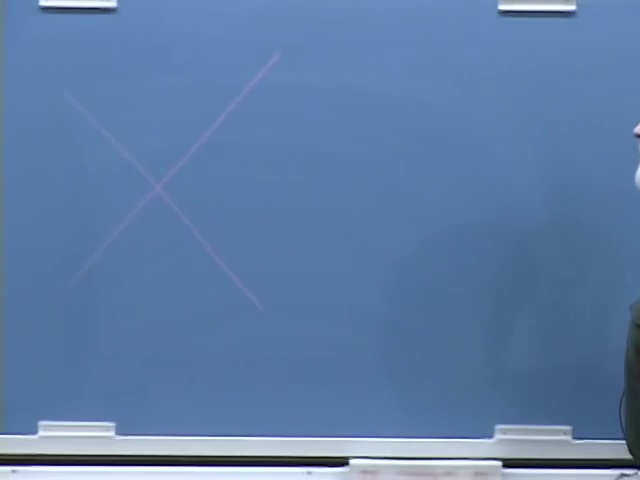
\includegraphics[width=0.68\textwidth]{lecture_09_figure_02.png}
\caption{La température de Hawking \(T_H=1/(8\pi M)\) en unités naturelles.}
\lectureframe{00:08:12}
\end{figure}

Un trou noir plus massif est plus froid. Le cours l’explique en retraçant le parcours d’un photon typique à rebours. Les photons thermiques ont une énergie caractéristique \(E_\gamma\sim T_H\). Un photon qui atteint l’infini avec une énergie de l’ordre de \(M^{-1}\) avait une énergie locale bien plus grande près de l’horizon, là où il a été émis. Le décalage vers le rouge entre la couche proche de l’horizon et l’infini est plus prononcé pour un trou noir plus massif, d’où une température asymptotique plus basse.

\begin{classroomqa}
\audiencequestion{Si le temps de Schwarzschild se fige à l’horizon, faut-il suivre le photon qui est tombé au départ et a formé le trou noir ?\lecturetimestamp{00:04:19}}
\lecturerresponse{Pour répondre à la question de la température, suivons les photons émis vers l’extérieur. Ils partent à une fréquence locale très élevée, perdent de l’énergie en remontant et arrivent sous forme de rayonnement de Hawking. Le devenir du photon initialement tombé est une question distincte, qui concerne l’information.}
\end{classroomqa}

\section{La couche de Planck et l’horizon étiré}

Jusqu’à quelle distance peut-on se fier à la relation locale de l’équation~\eqref{eq:l09-local-temperature} ? Dans le cours, la longueur de Planck est considérée comme la plus petite distance ayant un sens dans la description semi-classique. Cela suggère l’existence d’une mince couche, située à peu près à une longueur de Planck à l’extérieur de l’horizon mathématique, remplie de fluctuations à l’échelle de Planck. Elle émet et absorbe continuellement.

La plupart des quanta émis ne s’échappent pas. Seuls ceux qui sont dirigés dans un cône sortant très étroit évitent de retomber. Les quanta émis dans des directions génériques reviennent vers l’horizon. Les excitations sortantes et entrantes entrent en collision et produisent des paires ainsi que d’autres particules ; en ce sens, la description stationnaire comporte une fine coquille de matière extrêmement chaude.

\begin{figure}[htbp]
\centering
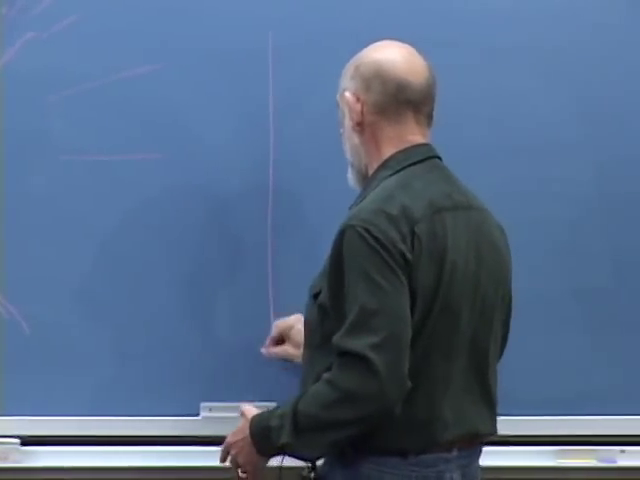
\includegraphics[width=0.74\textwidth]{lecture_09_figure_03.png}
\caption{Le cône d’échappement étroit du rayonnement proche de l’horizon. La plupart des quanta émis localement reviennent vers l’horizon.}
\lectureframe{00:11:38}
\end{figure}

Il existe une représentation complémentaire dans l’espace-temps. Loin d’un horizon, une fluctuation virtuelle peut être représentée schématiquement par une petite boucle fermée : une excitation particule-antiparticule apparaît puis disparaît avant de pouvoir devenir un état asymptotique. Près d’un horizon, une fluctuation peut chevaucher la frontière causale. Pour l’observateur extérieur, la partie située à l’extérieur ressemble à une particule émise par l’horizon puis réabsorbée. Une très petite fraction s’échappe et devient du rayonnement de Hawking.

\begin{classroomqa}
\audiencequestion{Dans le diagramme extérieur, une telle fluctuation s’étend-elle de \(t=-\infty\) à \(t=+\infty\) ?\lecturetimestamp{00:15:00}}
\lecturerresponse{L’horizon classique exact conduit à cette description d’apparence singulière. En pratique, nous le remplaçons par un horizon étiré, une surface de genre temps située à environ une longueur de Planck à l’extérieur. L’émission et la réabsorption ont alors lieu à des temps extérieurs finis.}
\end{classroomqa}

\begin{figure}[htbp]
\centering
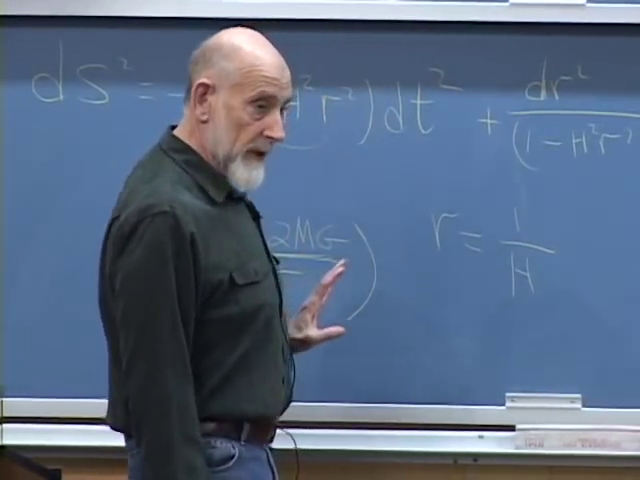
\includegraphics[width=0.72\textwidth]{lecture_09_figure_04.png}
\caption{L’horizon classique et l’horizon étiré voisin utilisé dans la description extérieure.}
\lectureframe{00:15:52}
\end{figure}

L’horizon étiré n’est pas une nouvelle frontière invariante. C’est une surface effective placée à l’endroit où la géométrie semi-classique cesse d’être fiable. Les fluctuations quantiques de la matière et de la géométrie elle-même brouillent la position exacte à l’échelle de Planck. Cette construction regroupe cette incertitude dans une surface où la description extérieure reste finie.

Rien dans cet argument local n’indique si l’horizon appartient à un trou noir ou à un univers en accélération. C’est le lien avec l’espace de de Sitter.

\section{L’espace de de Sitter en coordonnées en expansion}

Le cours proprement dit commence par le feuilletage spatialement plat de l’espace-temps de de Sitter,
\begin{equation}
ds^2=-dt^2+e^{2Ht}d\mathbf{x}^2,
\qquad
d\mathbf{x}^2=dx^2+dy^2+dz^2.
\label{eq:l09-flat-slicing}
\end{equation}
La constante \(H\) est le taux d’expansion de de Sitter. Le facteur apparaît sous la forme \(e^{2Ht}\) parce que la métrique mesure le carré des distances ; un intervalle de coordonnées fixe a pour longueur physique
\begin{equation}
D(t)=e^{Ht}\lvert\Delta\mathbf{x}\rvert.
\end{equation}

\begin{figure}[htbp]
\centering
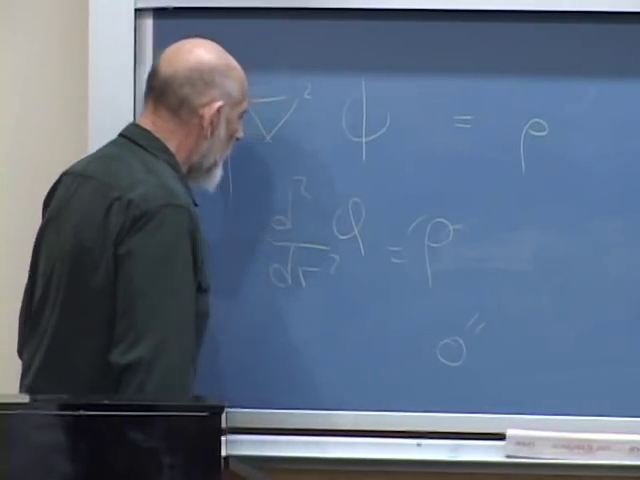
\includegraphics[width=0.78\textwidth]{lecture_09_figure_05.png}
\caption{La métrique de de Sitter en expansion exponentielle dans des coordonnées plates.}
\lectureframe{00:18:50}
\end{figure}

Ces coordonnées rendent l’expansion manifeste, mais placent l’infini futur à une distance infinie vers le haut de la page. Pour le faire apparaître au tableau, introduisons le temps conforme
\begin{equation}
\eta=-\frac{1}{H}e^{-Ht},
\qquad
-\infty<\eta<0.
\label{eq:l09-conformal-time}
\end{equation}
On a alors
\begin{equation}
dt=\frac{d\eta}{-H\eta},
\qquad
e^{Ht}=-\frac{1}{H\eta},
\end{equation}
et l’équation~\eqref{eq:l09-flat-slicing} devient
\begin{equation}
ds^2=\frac{1}{H^2\eta^2}
\left(-d\eta^2+d\mathbf{x}^2\right).
\label{eq:l09-conformal-metric}
\end{equation}
Lorsque \(t\to+\infty\), \(\eta\to0^{-}\). Un temps propre infini est ainsi comprimé sur la ligne horizontale finie \(\eta=0\).

\editorialnote{La transformation du temps est corrigée plusieurs fois pendant qu’elle est écrite au tableau. L’équation~\eqref{eq:l09-conformal-time} donne la forme cohérente : le début du temps cosmique correspond à \(\eta\to-\infty\) et l’infini futur à \(\eta\to0^{-}\).}

\begin{figure}[htbp]
\centering
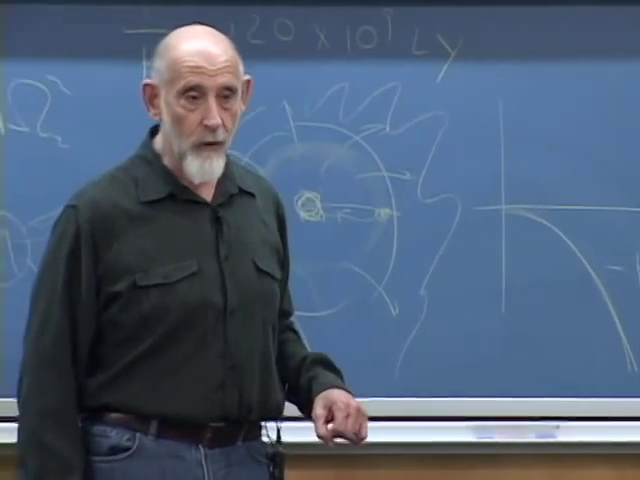
\includegraphics[width=0.82\textwidth]{lecture_09_figure_06.png}
\caption{La transformation vers le temps conforme et la métrique conformément plate.}
\lectureframe{00:21:24}
\end{figure}

Le facteur conforme multiplie les termes temporel et spatial ; il ne modifie donc pas les directions de genre nul. Pour un rayon lumineux radial,
\begin{equation}
ds^2=0
\quad\Longrightarrow\quad
-d\eta^2+dx^2=0
\quad\Longrightarrow\quad
\frac{dx}{d\eta}=\pm1.
\label{eq:l09-null-rays}
\end{equation}
La lumière se déplace donc à \(45^\circ\) dans le diagramme conforme. C’est ce qui rend ce changement de coordonnées utile : l’accessibilité causale devient visible.

\section{Le domaine causal d’un observateur}

Imaginons un observateur dont la ligne d’univers se prolonge pendant un temps propre infini. Sur le diagramme compactifié, elle aboutit en un point de \(\eta=0\). Tout signal que l’observateur peut recevoir se trouve dans le cône de lumière passé de ce point terminal. Les événements situés hors du cône ne peuvent jamais communiquer avec l’observateur, aussi longtemps qu’il attende.

\begin{figure}[htbp]
\centering
\includegraphics[width=0.78\textwidth]{lecture_09_figure_07.png}
\caption{Le cône de lumière passé limite d’un observateur dans les coordonnées conformes de de Sitter.}
\lectureframe{00:24:38}
\end{figure}

Un second observateur a un cône différent. Leurs domaines accessibles se recoupent, mais aucun des deux ne couvre tout l’espace-temps. Pour la suite de l’argument, adoptons le point de vue du premier observateur et appelons domaine causal de l’observateur ce cône de lumière passé.

Le dessin semble montrer que le domaine se rétrécit vers le futur, mais la largeur en coordonnées n’est pas une distance propre. Sur une tranche à temps constant \(\eta\), le carré de la distance physique entre l’observateur situé en \(x=0\) et l’horizon situé en \(x=\Delta x\) est
\begin{equation}
D^2=\frac{(\Delta x)^2}{H^2\eta^2}.
\label{eq:l09-horizon-distance-start}
\end{equation}
L’horizon est une droite de genre nul à \(45^\circ\) qui se termine en \(\eta=0\) ; par conséquent,
\begin{equation}
\Delta x=\lvert\eta\rvert.
\end{equation}
La substitution donne
\begin{equation}
D_{\rm hor}^2=\frac{1}{H^2},
\qquad
D_{\rm hor}=\frac{1}{H}.
\label{eq:l09-horizon-radius}
\end{equation}
La séparation en coordonnées diminue, mais le facteur conforme croît exactement de manière à compenser cette diminution. Le rayon propre de l’horizon est constant.

\begin{figure}[htbp]
\centering
\includegraphics[width=0.80\textwidth]{lecture_09_figure_08.png}
\caption{Dérivation au tableau qui transforme l’intervalle de coordonnées décroissant en la distance propre constante \(H^{-1}\).}
\lectureframe{00:28:42}
\end{figure}

\section{Le domaine statique}

Un rayon d’horizon constant suggère d’utiliser des coordonnées adaptées à l’observateur central. Sans dériver la transformation de coordonnées, le cours donne le résultat :
\begin{equation}
ds^2=
-\left(1-H^2r^2\right)d\tau^2
+\frac{dr^2}{1-H^2r^2}
+r^2d\Omega_2^2.
\label{eq:l09-static-patch}
\end{equation}
Les coefficients dépendent de \(r\), et non de \(\tau\). Cette carte couvre le domaine statique de l’observateur,
\begin{equation}
0\le r<\frac{1}{H}.
\end{equation}

\begin{figure}[htbp]
\centering
\includegraphics[width=0.88\textwidth]{lecture_09_figure_09.png}
\caption{La métrique du domaine statique de de Sitter et sa comparaison avec le facteur de Schwarzschild.}
\lectureframe{00:34:22}
\end{figure}

La ressemblance avec la métrique de Schwarzschild est immédiate :
\begin{equation}
f_{\rm dS}(r)=1-H^2r^2,
\qquad
f_{\rm Schw}(r)=1-\frac{2G_NM}{r}.
\end{equation}
Dans les deux cas, l’horizon en coordonnées statiques se trouve là où \(f(r)=0\). Pour de Sitter,
\begin{equation}
1-H^2r^2=0
\quad\Longrightarrow\quad
r_H=H^{-1}.
\end{equation}
La carte y est singulière, tout comme les coordonnées de Schwarzschild le sont à l’horizon d’un trou noir. Les géométries globales diffèrent néanmoins sur un point important. L’observateur d’un trou noir se tient à l’extérieur et regarde vers l’intérieur ; celui de de Sitter se tient à l’intérieur et regarde vers l’extérieur.

\begin{classroomqa}
\audiencequestion{Comment la géométrie peut-elle être statique alors que des particules en chute libre s’éloignent les unes des autres dans un univers en expansion exponentielle ?\lecturetimestamp{00:36:06}}
\lecturerresponse{Statique ne signifie pas que chaque particule reste immobile. Cela signifie que les coefficients de la métrique et le résultat d’une expérience répétée ne dépendent pas de l’heure à laquelle elle commence. Libérez deux particules maintenant : elles accélèrent en s’éloignant l’une de l’autre ; répétez la même expérience plus tard, et le même mouvement se produit.}
\end{classroomqa}

\begin{classroomqa}
\audiencequestion{Les deux particules qui s’éloignent l’une de l’autre se voient-elles mutuellement avec un décalage vers le rouge ?\lecturetimestamp{00:38:34}}
\lecturerresponse{Oui. L’augmentation de leur séparation produit un décalage relatif vers le rouge, même si la métrique adaptée à l’observateur est indépendante du temps.}
\end{classroomqa}

\section{La température observée de l’intérieur}

Les structures proches de l’horizon de Schwarzschild et de celui de de Sitter sont localement équivalentes. L’horizon de de Sitter émet donc des quanta thermiques et en réabsorbe. Un photon rare se propage vers l’intérieur jusqu’à l’observateur central, en perdant de l’énergie à mesure qu’il remonte le potentiel du domaine statique. La température de Gibbons--Hawking mesurée au centre est
\begin{equation}
T_{\rm dS}=\frac{H}{2\pi}
\label{eq:l09-de-sitter-temperature}
\end{equation}
en unités naturelles. Un thermomètre stationnaire au rayon \(r\) indique la valeur décalée vers le rouge selon Tolman
\begin{equation}
T_{\rm local}(r)=
\frac{T_{\rm dS}}{\sqrt{1-H^2r^2}},
\label{eq:l09-tolman}
\end{equation}
qui diverge lorsque \(r\to H^{-1}\) et se ramène, près de l’horizon, à l’équation~\eqref{eq:l09-local-temperature}.

\editorialnote{Le cours obtient l’échelle à partir de la distance à l’horizon et du décalage vers le rouge, sans écrire explicitement les équations~\eqref{eq:l09-de-sitter-temperature} et \eqref{eq:l09-tolman}. Elles donnent la normalisation standard de cet argument.}

Pour l’accélération observée à l’époque actuelle, le cours utilise l’estimation de période
\begin{equation}
H^{-1}\sim 20\times10^9\ {\rm light\ years}.
\label{eq:l09-lecture-horizon-estimate}
\end{equation}
Un photon typique de l’horizon a alors une longueur d’onde comparable à des milliards d’années-lumière. Il ne s’agit pas du rayonnement du fond diffus cosmologique : il est bien plus froid.

L’expérience de pensée opérationnelle met en scène une canne à pêche à l’échelle cosmologique. Alice reste en \(r=0\), fixe un thermomètre à une très longue ligne qui transmet aussi des données, puis laisse la répulsion cosmique emporter l’instrument vers l’extérieur. Elle l’arrête juste avant l’horizon, attend le retour du signal et constate une température locale élevée. Le thermomètre placé à côté d’elle, au centre, indique la faible valeur \(H/(2\pi)\). Un même horizon permet ces deux mesures, car elles sont effectuées à des potentiels gravitationnels différents.

\section{Franchir l’horizon}

La description classique depuis l’extérieur rappelle le récit habituel du trou noir. Bob, au centre, regarde Alice s’éloigner. Ses signaux subissent un décalage vers le rouge de plus en plus marqué et lui parviennent de plus en plus lentement ; elle semble s’aplatir contre l’horizon, puis finit par s’effacer. Une voyageuse qui arrive plus tard, Jane, apparaît comme une nouvelle couche, plus fine, dans un empilement sédimentaire près de la frontière.

\begin{classroomqa}
\audiencequestion{De notre point de vue, les objets franchissent-ils un jour l’horizon cosmique ?\lecturetimestamp{00:45:30}}
\lecturerresponse{Pas dans la description classique de l’observateur statique. Leurs signaux subissent un décalage vers le rouge et s’éteignent, tandis que leur position apparente se rapproche de l’horizon. Dans leur propre description en chute libre, toutefois, ils le franchissent sans rencontrer de surface singulière localement.}
\end{classroomqa}

\begin{classroomqa}
\audiencequestion{L’horizon n’est-il chaud que pour les observateurs qui restent tout près sans le franchir ? Un observateur en chute libre ne se fait pas cuire simplement en le traversant, n’est-ce pas ?\lecturetimestamp{00:48:27}}
\lecturerresponse{Alice franchit l’horizon sans heurt dans son propre référentiel. La température extrême appartient à la description stationnaire. Si Bob insiste pour observer Alice toujours plus près de l’horizon, il doit l’éclairer avec des longueurs d’onde toujours plus courtes. Le microscope de Heisenberg ainsi mis en œuvre dépose alors assez d’énergie pour cuire ce qu’il cherche à observer.}
\end{classroomqa}

Il ne s’agit pas d’une contradiction entre deux événements locaux. L’observateur stationnaire et l’observateur en chute libre effectuent des mesures radicalement différentes. La complémentarité des horizons demande comment ces deux descriptions peuvent être valides sans permettre à un même observateur de comparer directement des informations en double.

\section{Un modèle newtonien de la répulsion du vide}

À ce stade, un étudiant demande ce qui remplace le puits gravitationnel du trou noir. Susskind construit une réponse au moyen d’un modèle newtonien. Soit \(\phi\) le potentiel gravitationnel ; l’accélération d’une particule test est alors
\begin{equation}
\mathbf{a}=-\boldsymbol{\nabla}\phi.
\end{equation}
Pour une matière ordinaire non relativiste, l’équation de Poisson est
\begin{equation}
\nabla^2\phi=4\pi G_N\rho.
\label{eq:l09-poisson}
\end{equation}

\begin{classroomqa}
\audiencequestion{Si les effets du trou noir proviennent de son puits gravitationnel, quelle est la source correspondante dans l’espace de de Sitter ?\lecturetimestamp{00:49:36}}
\lecturerresponse{L’énergie du vide elle-même fournit une source gravitationnelle uniforme dans l’espace. Dans une description newtonienne, elle produit un potentiel quadratique plutôt qu’un puits en \(1/r\).}
\end{classroomqa}

\begin{figure}[htbp]
\centering
\includegraphics[width=0.78\textwidth]{lecture_09_figure_10.png}
\caption{L’équation de Poisson et la forme schématique de la dérivée seconde radiale utilisée dans le cours.}
\lectureframe{00:51:38}
\end{figure}

Au tableau, la normalisation, les termes associés à la mesure sphérique, la pression et, dans un premier temps, même le signe global sont omis. Le problème se réduit à
\begin{equation}
\frac{d^2\phi}{dr^2}\sim H^2.
\end{equation}
L’inférence essentielle est qu’une source constante donne une fonction quadratique. Avec le signe correspondant à la répulsion de de Sitter,
\begin{equation}
\phi_{\rm dS}(r)=-\frac{1}{2}H^2r^2,
\qquad
a_r=-\frac{d\phi_{\rm dS}}{dr}=H^2r.
\label{eq:l09-de-sitter-potential}
\end{equation}
L’accélération est dirigée vers l’extérieur et croît linéairement avec la distance. La résolution de \(\ddot r=H^2r\) donne
\begin{equation}
r(\tau)=A e^{H\tau}+B e^{-H\tau},
\end{equation}
La branche croissante reproduit ainsi la séparation exponentielle.

\begin{figure}[htbp]
\centering
\includegraphics[width=0.76\textwidth]{lecture_09_figure_11.png}
\caption{L’équation à source uniforme et le potentiel quadratique de de Sitter.}
\lectureframe{00:53:32}
\end{figure}

\editorialnote{En relativité générale, l’accélération dans le champ faible d’un fluide homogène dépend de \(\rho+3p\), et non de \(\rho\) seul. L’énergie du vide vérifie \(p=-\rho\), donc \(\rho+3p=-2\rho\) et l’accélération est répulsive. L’équation~\eqref{eq:l09-de-sitter-potential} donne le résultat de de Sitter correctement normalisé ; le calcul au tableau ne suit volontairement que la dépendance quadratique et le signe.}

Plaçons une masse ordinaire \(M\) au centre. Le potentiel qualitatif devient
\begin{equation}
\phi(r)=-\frac{G_NM}{r}-\frac{1}{2}H^2r^2,
\label{eq:l09-combined-potential}
\end{equation}
et l’accélération radiale vaut
\begin{equation}
a_r=-\frac{G_NM}{r^2}+H^2r.
\end{equation}
À faible \(r\), l’attraction locale l’emporte ; à grand \(r\), c’est la répulsion du vide. L’équilibre se produit à
\begin{equation}
r_\ast=\left(\frac{G_NM}{H^2}\right)^{1/3}.
\label{eq:l09-turnaround}
\end{equation}
C’est une version claire du maximum du potentiel évoqué dans le cours. Elle explique qualitativement pourquoi des systèmes gravitationnellement liés proches peuvent rester ensemble, alors que les galaxies suffisamment éloignées s’éloignent en accélérant.

\begin{figure}[htbp]
\centering
\includegraphics[width=0.78\textwidth]{lecture_09_figure_12.png}
\caption{Attraction ordinaire en \(1/r\) combinée au potentiel quadratique inversé de de Sitter.}
\lectureframe{00:58:20}
\end{figure}

\begin{classroomqa}
\audiencequestion{Les forces ordinaires comptent-elles toujours, ou la répulsion du vide finit-elle par déchirer tous les îlots de matière ?\lecturetimestamp{00:57:29}}
\lecturerresponse{Il faut tenir compte de toutes les forces. À des échelles suffisamment petites, les liaisons électromagnétiques et la gravité locale dominent. La répulsion du vide ne devient importante qu’à des distances immenses, déterminées par \(H^{-1}\) et par l’échelle d’équilibre correspondant à la masse liée.}
\end{classroomqa}

\section{Une source, plusieurs noms}

La discussion s’interrompt maintenant pour préciser la terminologie. Dans le modèle utilisé ici, l’énergie du vide, la constante cosmologique et l’énergie noire ne sont pas trois substances qui s’additionnent. Ce sont trois descriptions d’une même source, caractérisée par \(w=-1\). On peut parler d’un terme constant dans l’équation d’Einstein, d’une densité d’énergie du vide invariante de Lorentz ou de la composante qui entraîne l’accélération tardive de l’expansion.

\begin{classroomqa}
\audiencequestion{La source newtonienne uniforme et l’énergie quantique du vide sont-elles présentes toutes les deux comme des effets distincts ?\lecturetimestamp{00:59:14}}
\lecturerresponse{Non. La densité uniforme est le modèle newtonien de cette même source. L’énergie du vide, la constante cosmologique et, dans ce cours, l’énergie noire désignent une seule composante physique.}
\end{classroomqa}

\begin{classroomqa}
\audiencequestion{Le même phénomène admet-il donc une description classique et une description quantique ?\lecturetimestamp{01:00:32}}
\lecturerresponse{Son origine microscopique est peut-être quantique, tout comme une partie de la masse de l’électron a une origine quantique. Une fois la densité d’énergie effective connue, elle intervient comme une source ordinaire dans les équations classiques de la gravitation. Nous ignorons l’origine ultime de la valeur observée.}
\end{classroomqa}

En unités de Planck, la densité d’énergie du vide observée est extraordinairement faible,
\begin{equation}
\rho_\Lambda\sim10^{-123}\rho_{\rm Pl},
\label{eq:l09-planck-smallness}
\end{equation}
à un facteur de convention près pour la densité de Planck. Cette petitesse est au cœur du problème de la constante cosmologique. C’est aussi pourquoi l’horizon est si grand : en quatre dimensions,
\begin{equation}
H^2=\frac{8\pi G_N}{3}\rho_\Lambda,
\qquad
r_H=H^{-1}.
\end{equation}
Si \(H\) était plus grand, l’horizon serait plus petit, la température centrale de de Sitter serait plus élevée et l’accélération répulsive \(H^2r\) serait plus forte.

\begin{classroomqa}
\audiencequestion{La petitesse de la constante cosmologique est-elle liée à la constante de Planck et aux fluctuations quantiques ?\lecturetimestamp{01:03:27}}
\lecturerresponse{La comparaison la plus claire se fait en unités de Planck sans dimension, où \(G_N=\hbar=c=1\). Dans ces unités, la densité du vide est inférieure d’environ \(123\) ordres de grandeur à la densité de Planck naturelle. Expliquer cette hiérarchie est l’une des grandes énigmes de la physique fondamentale.}
\end{classroomqa}

\begin{classroomqa}
\audiencequestion{L’énergie du vide doit-elle être une constante cosmologique exactement constante ? La composante responsable de l’accélération pourrait-elle diminuer et finir par tendre vers zéro ?\lecturetimestamp{01:04:52}}
\lecturerresponse{C’est une autre possibilité cohérente : un champ dynamique d’énergie noire pourrait varier au cours du temps. Le cours retient le cas constant parce que les observations disponibles à l’époque favorisaient de plus en plus un comportement proche de celui d’une constante cosmologique, et non parce que toutes les autres possibilités avaient été démontrées impossibles.}
\end{classroomqa}

\section{L’astronomie dans un avenir lointain}

Dans un univers asymptotiquement de Sitter, les structures qui ne sont pas gravitationnellement liées finissent par franchir l’horizon de l’observateur. Le rayonnement de fond cosmologique tombe sous le seuil de détection. Les galaxies lointaines disparaissent. Un astronome encore en vie pourrait ne voir qu’un îlot gravitationnel local fusionné, au milieu d’un domaine autrement sombre.

\begin{classroomqa}
\audiencequestion{Sans télescope, quelqu’un remarquerait-il seulement la disparition des galaxies lointaines ?\lecturetimestamp{01:06:17}}
\lecturerresponse{Probablement pas. La difficulté véritable est plus profonde : même avec des instruments avancés, les observateurs du futur pourraient ne plus disposer des traceurs lointains ni du fond diffus cosmologique qui nous permettent aujourd’hui de déduire l’expansion.}
\end{classroomqa}

L’ancienne représentation d’un univers composé d’îles pourrait alors sembler convaincante. Le paradoxe d’Olbers n’imposerait pas une autre conclusion, car il suppose une population infinie, statique et uniforme de sources lumineuses ; l’observateur du futur ne verrait que le nombre fini d’étoiles de l’îlot local. L’énergie noire ne crée pas continuellement des galaxies de remplacement à partir du vide.

Dans l’espace de de Sitter exact, l’horizon ne se rétrécit pas autour de la galaxie locale. Son rayon physique reste égal à \(H^{-1}\), une valeur immensément supérieure à la taille d’une galaxie. Ce qui disparaît, c’est la matière non liée qui passe au-delà de cette frontière causale fixe.

\begin{classroomqa}
\audiencequestion{Les étoiles éjectées de la galaxie pourraient-elles servir de corps tests pour détecter la géométrie à grande échelle ?\lecturetimestamp{01:11:25}}
\lecturerresponse{Pendant un certain temps, oui. Les objets éjectés et les signaux lumineux couvrant de grandes distances pourraient sonder la géométrie. Mais l’effet ne devient appréciable qu’à des distances de l’ordre d’une fraction importante d’un milliard d’années-lumière, si bien que l’expérience prendrait un temps cosmologique.}
\end{classroomqa}

\begin{classroomqa}
\audiencequestion{Comment savons-nous qu’un horizon lointain ne nous a pas déjà caché la majeure partie de l’Univers ?\lecturetimestamp{01:11:45}}
\lecturerresponse{Nous voyons déjà assez de galaxies, de décalages vers le rouge et de rayonnement de fond pour mesurer l’expansion et reconstruire la géométrie à grande échelle. Les observateurs futurs privés de ces traceurs auraient beaucoup plus de mal à en déduire la géométrie.}
\end{classroomqa}

\begin{classroomqa}
\audiencequestion{Si l’horizon se trouvait juste au-delà d’Andromède, sa présence serait-elle manifeste ?\lecturetimestamp{01:12:19}}
\lecturerresponse{Oui. Un horizon aussi petit exigerait un \(H\) bien plus grand, et la répulsion qui en résulterait modifierait fortement le mouvement d’Andromède. La valeur mesurée place au contraire l’horizon asymptotique à une échelle immensément plus grande.}
\end{classroomqa}

\begin{classroomqa}
\audiencequestion{De nouveaux big bangs pourraient-ils se produire au-delà de notre horizon ?\lecturetimestamp{01:13:25}}
\lecturerresponse{Les événements au-delà de l’horizon ne sont visibles ni par nous ni par nos descendants. Une possibilité connexe, mais formulée plus précisément, sera présentée plus loin dans le cours : la nucléation de bulles dans l’inflation éternelle.}
\end{classroomqa}

Avec des fusées, des horloges et plusieurs milliards d’années, les observateurs du futur pourraient envoyer des explorateurs à travers une grande partie du domaine et en reconstruire la métrique. À l’échelle ordinaire d’un laboratoire ou d’une civilisation, toutefois, l’effet est presque inaccessible. Cette distinction corrige l’affirmation trop forte selon laquelle l’expansion serait impossible à découvrir : la mesure est très éloignée dans la pratique, mais pas interdite en principe.

\begin{classroomqa}
\audiencequestion{Les explorateurs du futur pourraient-ils déterminer la géométrie bien plus tôt qu’en attendant une récurrence thermique ?\lecturetimestamp{01:21:40}}
\lecturerresponse{Certainement. Une récurrence n’est pas la mesure proposée. En échangeant des signaux lumineux sur des distances de plusieurs milliards d’années-lumière, les explorateurs pourraient cartographier le domaine statique sur une échelle de temps bien plus courte, quoique toujours cosmologique.}
\end{classroomqa}

\begin{classroomqa}
\audiencequestion{Le décalage vers le rouge effacerait-il toutes les informations rapportées par de tels explorateurs ?\lecturetimestamp{01:23:24}}
\lecturerresponse{Non, s’ils sondent des échelles bien inférieures à celle de l’horizon. Une base de l’ordre du milliard d’années-lumière est déjà sensible à l’expansion tout en ne produisant qu’un décalage vers le rouge modéré. L’expérience est limitée surtout par sa durée immense.}
\end{classroomqa}

\section{Entropie finie et récurrence}

La région statique n’est pas vide au sens thermodynamique. Son horizon a une aire
\begin{equation}
A_H=4\pi H^{-2},
\end{equation}une température \(T_{\rm dS}=H/(2\pi)\), et une entropie
\begin{equation}
S_{\rm dS}=\frac{A_H}{4G_N}
=\frac{\pi}{G_NH^2}
\label{eq:l09-de-sitter-entropy}
\end{equation}en unités \(\hbar=c=k_B=1\). Cette entropie est finie. On peut donc se représenter, avec les précautions qui s’imposent, la région statique comme une cavité thermique d’entropie finie, dont les excitations sont concentrées près de l’horizon dans la description stationnaire.

Une boîte ordinaire de gaz à l’équilibre semble dépourvue de caractéristiques à courte échelle de temps, mais la mécanique statistique n’interdit pas les fluctuations. Si un macroétat présente un déficit d’entropie \(\Delta S\)par rapport à l’équilibre, sa probabilité est approximativement
\begin{equation}
P\sim e^{-\Delta S}.
\label{eq:l09-fluctuation-probability}
\end{equation}
Le temps d’attente correspondant croît comme
\begin{equation}
t\sim t_0 e^{\Delta S}.
\end{equation}
Pour un système fini, le temps nécessaire pour revenir à un état arbitrairement proche d’un état antérieur est le temps de récurrence de Poincaré,
\begin{equation}
t_{\rm rec}\sim H^{-1}e^{S_{\rm dS}}.
\label{eq:l09-recurrence}
\end{equation}
Puisque \(S_{\rm dS}\) de notre horizon est de l’ordre de \(10^{120}\), le cours donne pour cette échelle \(e^{10^{120}}\). Que le facteur multiplicatif soit exprimé en années, en temps de Hubble ou en unités microscopiques n’a aucune importance face à la double exponentielle.

\begin{figure}[htbp]
\centering
\includegraphics[width=0.76\textwidth]{lecture_09_figure_13.png}
\caption{Discussion sur la récurrence, avec au tableau l’énorme échelle exponentielle du temps d’attente.}
\lectureframe{01:16:24}
\end{figure}

Avant une telle récurrence, les fluctuations de moindre ampleur sont beaucoup plus fréquentes. Les molécules d’une pièce pourraient toutes se rassembler dans un coin ; un vortex complexe pourrait se former brièvement ; dans la hiérarchie plaisante évoquée pendant le cours, le mouvement thermique pourrait assembler un éléphant. Plus le déficit d’entropie requis est faible, moins la fluctuation est coûteuse.

\begin{classroomqa}
\audiencequestion{Les récurrences de Poincaré sont-elles spécifiquement une conséquence de la mécanique quantique ?\lecturetimestamp{01:25:44}}
\lecturerresponse{Non. Les récurrences et les fluctuations rares apparaissent déjà en mécanique statistique classique. Leur application à l’espace de de Sitter s’inscrit dans notre cadre physique actuel, qui pourrait être révisé un jour ; mais la thermodynamique et le raisonnement statistique comptent parmi les structures les plus robustes que nous connaissions.}
\end{classroomqa}

La signification même de la probabilité pourrait s’approfondir dans une théorie future. Susskind ne prétend pas le contraire. Son propos, plus limité, est que renoncer à la mécanique statistique simplement parce que ses implications à long terme sont étranges reviendrait à abandonner l’un des principes organisateurs les mieux éprouvés de la physique.

\section{Cerveaux de Boltzmann et observateurs typiques}

Supposons qu’une fluctuation thermique crée un état entier semblable à celui d’un big bang. Cela exige une diminution d’entropie énorme. Une fluctuation qui produit un système solaire coûte moins ; une Terre déjà chaude coûte moins encore. Si la seule exigence est la présence d’un observateur, la fluctuation la moins coûteuse pourrait ne créer qu’un cerveau fonctionnel doté de souvenirs apparents. Un tel observateur hypothétique est appelé cerveau de Boltzmann.

La question n’est pas de savoir si une fluctuation extraordinaire est logiquement possible. Elle est de savoir si un modèle cosmologique prédit que presque tous les observateurs sont de telles fluctuations. Nous tirons des conclusions de nos observations en supposant que nous ne sommes pas extraordinairement atypiques. Une théorie dans laquelle les observateurs ordinaires, dotés d’une histoire cosmique cohérente, sont exponentiellement moins nombreux que des cerveaux thermiques isolés compromet cette inférence.

Le problème des cerveaux de Boltzmann désigne donc un critère quantitatif de cohérence. On compare l’abondance attendue des observateurs ordinaires à celle des observateurs issus de fluctuations. Si ces derniers dominent, il faut soit que le vide se désintègre avant leur prolifération, soit modifier la mesure, soit réexaminer les hypothèses cosmologiques.

Une question antérieure sur un lien entre ultraviolet--et infrarouge est explicitement laissée de côté. L’argument de récurrence ne dépend pas de la résolution de cette question distincte.

\section{Inflation éternelle et univers-bulles}

Le cours présente ensuite, sans chercher à en donner une dérivation complète, un second problème de probabilité. Un vide de de Sitter métastable peut nucléer une bulle où l’énergie du vide est plus faible. La paroi de la bulle s’étend, et son intérieur peut évoluer en un univers de Friedmann--Robertson--Walker ouvert. Pendant ce temps, la région inflationnaire qui l’entoure continue de s’étendre et nuclée d’autres bulles.

\begin{figure}[htbp]
\centering
\includegraphics[width=0.74\textwidth]{lecture_09_figure_14.png}
\caption{Une bulle de plus faible énergie du vide dessinée à l’intérieur d’un arrière-plan de de Sitter en inflation.}
\lectureframe{01:29:38}
\end{figure}

Le trait essentiel est la croissance exponentielle du nombre de régions. Du nouveau volume physique se crée plus vite que les bulles n’en éliminent ; le nombre de régions-bulles croît donc sans limite. Des bulles différentes peuvent se stabiliser dans des états de basse énergie différents et présenter, par conséquent, des lois physiques effectives différentes.

Pour mettre en évidence la difficulté statistique, Susskind quitte d’abord la cosmologie et considère une population humaine en croissance exponentielle, avec des ressources finies mais inconnues. Supposons que les observateurs soient typiques parmi tous ceux qui vivront jamais. Si la population double à chaque génération puis disparaît, la moitié des individus vivent dans la dernière génération, les trois quarts dans les deux dernières et les sept huitièmes dans les trois dernières :
\begin{equation}
f_n=1-2^{-n}.
\label{eq:l09-last-generations}
\end{equation}
La typicité nous situerait alors inconfortablement près de la fin, même si nous ne savons rien de la quantité totale de ressources. Il ne s’agit pas d’une prédiction fiable de l’extinction humaine, mais d’un avertissement : avec une croissance exponentielle, le décompte est dominé par la coupure.

L’exemple du lancer de pièce énonce plus clairement l’hypothèse habituelle de typicité. Si de nombreux expérimentateurs lancent chacun une pièce équilibrée \(N\)fois, l’immense majorité obtient
\begin{equation}
n_H=\frac{N}{2}+O(\sqrt{N}).
\end{equation}
Un observateur atypique devrait d’abord soupçonner un mauvais modèle ou une pièce truquée, plutôt que de supposer sans preuve qu’il se trouve dans une queue de distribution extraordinairement rare. La cosmologie probabiliste repose sur la même intuition de typicité, mais dans une population infinie, il lui faut une méthode de dénombrement bien définie.

\section{La frontière d’Escher et le problème de la mesure}

L’analogie géométrique de Susskind est \ M.\ C.\emph{Circle Limit IV}d’Escher : un disque pavé d’anges et de démons qui semblent rapetisser à mesure qu’ils s’approchent du bord. Dans la géométrie hyperbolique représentée par le dessin, ces figures sont équivalentes ; seule leur taille euclidienne apparente change sous l’effet de la projection.

\begin{figure}[htbp]
\centering
\includegraphics[width=0.76\textwidth]{lecture_09_figure_15.png}
\caption{Une représentation au tableau des figures d’Escher qui prolifèrent exponentiellement près d’une frontière circulaire.}
\lectureframe{01:37:54}
\end{figure}

Imaginons qu’Escher dispose d’un temps, d’une encre et d’une patience limités. Près du bord, il finit par s’arrêter, laissant peut-être certaines figures inachevées. Comme leur nombre croît exponentiellement avec le rayon hyperbolique, une couche périphérique d’épaisseur finie contient une fraction d’ordre un de toutes les figures dessinées. Environ la moitié peut se trouver dans la dernière couche, quelle que soit la distance à laquelle on repousse la coupure.

Demandons maintenant quel est le rapport entre les anges et les démons. Dans le motif infini idéal, la symétrie suggère une égalité un pour un. Dans tout dénombrement fini, cependant, une frontière légèrement différente peut inclure beaucoup plus de figures d’un type que de l’autre. Comme la majeure partie du décompte se trouve près de la frontière, une légère déformation de celle-ci modifie la réponse d’une quantité d’ordre un.

\begin{figure}[htbp]
\centering
\includegraphics[width=0.76\textwidth]{lecture_09_figure_16.png}
\caption{Dans un motif à croissance exponentielle, le décompte est dominé par la frontière de coupure.}
\lectureframe{01:43:06}
\end{figure}

La même ambiguïté apparaît dans l’inflation éternelle. On dénombre les univers-bulles bleus et roses jusqu’à une certaine coupure temporelle, puis on repousse celle-ci. Les deux décomptes divergent, et leur rapport peut dépendre fortement de ce que signifie \emph{temps}et de la façon dont on trace la surface de coupure. Une mesure de probabilité est une prescription qui régularise la population infinie et en extrait les probabilités relatives. Le fait que différentes prescriptions plausibles ne concordent pas constitue le problème de la mesure.

\begin{classroomqa}
\audiencequestion{Ce problème de coupure est-il lié à la renormalisation ?\lecturetimestamp{01:45:43}}
\lecturerresponse{Il y a une analogie. En théorie quantique des champs, on introduit un réseau ou une coupure ultraviolette, on l’affine, puis on cherche des grandeurs insensibles aux détails de la frontière du régulateur. Les cosmologistes espèrent pouvoir extraire de l’inflation éternelle des résultats tout aussi robustes, mais, dans le cadre discuté ici, aucune prescription aussi décisive n’est encore disponible.}
\end{classroomqa}

Il ne faut pas exagérer la portée de l’analogie. La renormalisation réussit lorsqu’un flot contrôlé permet d’identifier des observables indépendantes du régulateur. Le problème de la mesure tient précisément au fait que les questions invariantes analogues et la procédure de passage à la limite restent mal définies. Dire que nous posons peut-être la mauvaise question n’est pas une solution tant que la bonne question n’est pas formulée.

\begin{classroomqa}
\audiencequestion{Cette image des bulles correspond-elle au même phénomène que l’inflation dans notre univers primordial ?\lecturetimestamp{01:48:19}}
\lecturerresponse{Le lien est étroit. Dans l’inflation éternelle, l’arrière-plan parent continue son inflation tandis que l’intérieur des bulles évolue selon sa propre cosmologie. Notre univers observable pourrait se trouver dans une telle région.}
\end{classroomqa}

\section{Peut-on observer des collisions entre bulles ?}

Lorsque deux bulles se rencontrent, leurs énergies du vide ne s’additionnent pas simplement. Une paroi de domaine sépare des régions correspondant à des états différents du vide, et la géométrie de cette paroi détermine ce que chaque côté peut observer. Selon la position de la collision par rapport à notre cône de lumière passé, sa trace peut être cachée ou visible.

\begin{classroomqa}
\audiencequestion{Que se passe-t-il lorsque deux bulles de vide entrent en collision ?\lecturetimestamp{01:52:07}}
\lecturerresponse{La collision crée une géométrie de paroi de domaine dont le comportement dépend des deux vides et de la tension de la paroi. Si les conditions causales sont favorables, la perturbation peut atteindre notre région observable et y laisser une signature anisotrope.}
\end{classroomqa}

Le cours évoque une région froide du fond diffus cosmologique comme candidate possible et mentionne la polarisation autour d’une structure circulaire comme critère distinctif. Cette hypothèse est présentée délibérément comme une possibilité, et non comme une détection. Une signature convaincante d’une collision révolutionnerait le domaine, car elle fournirait une preuve directe de l’existence de régions-bulles voisines et rendrait urgente la résolution expérimentale du problème de la mesure.

\begin{figure}[htbp]
\centering
\includegraphics[width=0.70\textwidth]{lecture_09_figure_17.png}
\caption{Une structure circulaire dans le ciel et son éventuel motif de polarisation dans le contexte des collisions de bulles.}
\lectureframe{01:50:22}
\end{figure}

\editorialnote{La discussion de la tache froide rend compte de l’état des observations et des propositions au moment du cours. Une anomalie de température ne constitue pas à elle seule une preuve de collision entre bulles ; il faudrait une signature détaillée et corrélée.}

\begin{classroomqa}
\audiencequestion{Les bulles sont-elles quadridimensionnelles, et quelle est la courbure spatiale de leur intérieur ?\lecturetimestamp{01:53:37}}
\lecturerresponse{Ce sont des régions de l’espace-temps, et non des bulles de savon tridimensionnelles évoluant dans un temps extérieur. Leur intérieur est généralement un univers FRW ouvert à courbure spatiale négative. Une collision perturbe cette géométrie, mais ne transforme pas simplement la courbure négative en courbure positive.}
\end{classroomqa}

\section{Ce que la théorie des cordes établit et ce qu’elle n’établit pas}

La discussion finale commence par une invitation à attribuer une probabilité à la validité de la théorie des cordes. Susskind refuse de donner un chiffre, car la proposition est trop ambiguë. Il distingue plutôt deux affirmations.

Premièrement, il existe une structure mathématique très fortement contrainte, qui combine mécanique quantique et gravitation. Elle a produit des résultats précis et de profondes identités mathématiques, et sa cohérence interne a résisté à un examen approfondi. Dans le vocabulaire informel du cours, il s’agit de \emph{théorie des cordes} avec un \(S\) majuscule. Les versions que l’on comprend le mieux reposent largement sur la supersymétrie.

Deuxièmement, le monde observé n’est pas supersymétrique aux énergies accessibles. Pour relier les constructions exactes supersymétriques à notre univers non supersymétrique, il faut briser la supersymétrie et recourir à un cadre plus vaste, qui n’est pas maîtrisé avec la même précision. Dans le vocabulaire du cours, cette extension espérée est \emph{théorie des cordes} avec un \(s\) minuscule.

\begin{classroomqa}
\audiencequestion{Peut-on attribuer une probabilité à la proposition selon laquelle la théorie des cordes est la théorie correcte de la nature ?\lecturetimestamp{01:54:18}}
\lecturerresponse{Pas de manière responsable sans préciser de quelle affirmation il s’agit. Les structures mathématiques exactes existent et incluent la gravité quantique, mais les modèles supersymétriques rigoureusement maîtrisés ne décrivent pas littéralement le monde que nous observons. La question de savoir si une extension plus vaste contient notre monde relève de convictions éclairées que peuvent avoir les physiciens, et non d’une probabilité numérique bien définie.}
\end{classroomqa}

L’analogie est celle de la mécanique avant que tout son appareil mathématique soit disponible. On pouvait connaître \(F=ma\)et la force en inverse du carré de la distance, tout en ne sachant résoudre que les orbites circulaires hautement symétriques. Le domaine soluble aurait été réel, sans constituer la théorie entière. De même, les constructions exactes de la théorie des cordes supersymétrique pourraient représenter une région particulière, exceptionnellement maniable, d’une structure plus vaste.

\begin{figure}[htbp]
\centering
\includegraphics[width=0.60\textwidth]{lecture_09_figure_18.png}
\caption{Le schéma emboîté du cours : des constructions supersymétriques de la théorie des cordes, rigoureusement maîtrisées, au sein d’un cadre conjectural plus vaste.}
\lectureframe{01:57:34}
\end{figure}

\begin{classroomqa}
\audiencequestion{Pourquoi ne pas simplement briser la supersymétrie dans la théorie exacte ?\lecturetimestamp{01:57:02}}
\lecturerresponse{De nombreuses constructions approchées étudient la brisure de supersymétrie, et les mathématiques supersymétriques sont bien connues. Ce qui manque précisément, c’est un socle non supersymétrique entièrement maîtrisé. On peut effectuer des calculs après avoir adopté les approximations usuelles sans toujours savoir vers quel objet exact ces approximations convergent.}
\end{classroomqa}

\begin{classroomqa}
\audiencequestion{La théorie supersymétrique exacte exclut-elle une extension plus vaste et moins symétrique qui contiendrait notre monde ?\lecturetimestamp{02:00:33}}
\lecturerresponse{Non. Elle établit que le monde observé n’est pas décrit par le seul secteur supersymétrique exact. Elle ne prouve ni ne réfute que ce secteur soit relié à une théorie plus vaste contenant une physique réaliste.}
\end{classroomqa}

\begin{classroomqa}
\audiencequestion{Les constructions de la théorie des cordes incluent-elles une brisure de symétrie analogue à celle de la physique des particules ?\lecturetimestamp{02:01:21}}
\lecturerresponse{Les travaux sur la brisure de supersymétrie sont nombreux, et l’on sait beaucoup de choses sur les mathématiques supersymétriques. Ce qui reste à résoudre, c’est la formulation précise et non perturbative qui intègre une brisure réaliste à la théorie complète, et non aux seules approximations maîtrisées.}
\end{classroomqa}

\begin{classroomqa}
\audiencequestion{La relativité restreinte est-elle postulée dans la théorie des cordes, ou en découle-t-elle comme une prédiction ?\lecturetimestamp{02:03:02}}
\lecturerresponse{Les règles fondamentales sont invariantes de Lorentz, même si un arrière-plan particulier rempli de matière peut sélectionner un référentiel de repos privilégié. La gravité est encore plus inévitable : le spectre des cordes contient une excitation sans masse de spin deux, dont les interactions sont celles d’un graviton.}
\end{classroomqa}

\begin{classroomqa}
\audiencequestion{La théorie des cordes est-elle compatible avec la relativité générale et l’indépendance vis-à-vis de l’arrière-plan ?\lecturetimestamp{02:04:11}}
\lecturerresponse{Sa dynamique gravitationnelle à basse énergie est compatible avec la relativité générale, et les arrière-plans locaux peuvent être modifiés dynamiquement. La subtilité tient aux conditions aux limites asymptotiques : elles définissent le problème lui-même et ne peuvent généralement pas être modifiées par une opération locale dans cet espace-temps.}
\end{classroomqa}

Le cours s’achève sur cette distinction entre un noyau mathématique robuste et une extrapolation physique inachevée. Il ne s’agit ni d’affirmer que le noyau est inutile, ni de prétendre que l’extrapolation est établie. C’est une indication de la limite actuelle du savoir exact.

\end{document}